%%%%%%%%%%%%%%%%%%%%%%%%%%%%%%%%%%%%%%%%%%%%%%%%%%%%%%%%%%%%%%%%%%%%%%%%%%%%%
%%% LaTeX-Rahmen fuer das Erstellen von Bachelorarbeiten
%%%%%%%%%%%%%%%%%%%%%%%%%%%%%%%%%%%%%%%%%%%%%%%%%%%%%%%%%%%%%%%%%%%%%%%%%%%%%

%%%%%%%%%%%%%%%%%%%%%%%%%%%%%%%%%%%%%%%%%%%%%%%%%%%%%%%%%%%%%%%%%%%%%%%%%%%%%
%%% allgemeine Einstellungen
%%%%%%%%%%%%%%%%%%%%%%%%%%%%%%%%%%%%%%%%%%%%%%%%%%%%%%%%%%%%%%%%%%%%%%%%%%%%%

\documentclass[twoside,12pt,a4paper]{report}
%\usepackage{reportpage}
\usepackage{epsf,ngerman}
\usepackage{graphics, graphicx}
\usepackage{latexsym}
\usepackage[margin=10pt,font=small,labelfont=bf]{caption}
\usepackage[utf8]{inputenc}     % Umlaute
\usepackage{wrapfig}
\usepackage{longtable}
\usepackage{qtree}
\usepackage{floatrow}
\usepackage{tabu}
\usepackage{diagbox}
\usepackage{rotating}
%\usepackage[ngerman]{babel} 
\usepackage{lscape}
\usepackage{csquotes}
\usepackage{amsmath}

\setcounter{tocdepth}{4}
\setcounter{secnumdepth}{4}

\usepackage{hyperref}
\hypersetup{
    colorlinks,
    citecolor=black,
    filecolor=black,
    linkcolor=black,
    urlcolor=black
}

\textwidth 14cm
\textheight 22cm
\topmargin 0.0cm
\evensidemargin 1cm
\oddsidemargin 1cm
%\footskip 2cm
\parskip0.5explus0.1exminus0.1ex

% Kann von Student auch nach pers\"onlichem Geschmack ver\"andert werden.
\pagestyle{headings}

\sloppy

\begin{document}

%%%%%%%%%%%%%%%%%%%%%%%%%%%%%%%%%%%%%%%%%%%%%%%%%%%%%%%%%%%%%%%%%%%%%%%%%%%%
%%% hier steht die neue Titelseite 
%%%%%%%%%%%%%%%%%%%%%%%%%%%%%%%%%%%%%%%%%%%%%%%%%%%%%%%%%%%%%%%%%%%%%%%%%%%%
 
\begin{titlepage}
 \begin{center}
  {\LARGE Eberhard Karls Universit"at T"ubingen}\\
  {\large Mathematisch-Naturwissenschaftliche Fakult"at \\
Wilhelm-Schickard-Institut f"ur Informatik\\[4cm]}
  {\huge Bachelorarbeit Informatik\\[2cm]}
  {\Large\bf Prädiktion des lexikalischen Wortakzentes durch Maschinelles Lernen\\[1.5cm]}
 {\large Stephan Biastoch}\\[0.5cm]
Sommersemester 2015\\[5cm]
\begin{center}{\small\bf Gutachter}\\[0.5cm]
{\large Dr. Alexandra Kirsch}\\
  {\footnotesize Wilhelm-Schickard-Institut f\"ur Informatik\\%
	Universit"at T"ubingen}	\end{center}
	
	%\begin{center}
%{\small\bf Betreuer}\\[0.5cm]
%{\large Name Betreuer}\\
%  {\footnotesize Adresse\\
%	Universit"at T"ubingen}\end{center}

  \end{center}
\end{titlepage}


%%%%%%%%%%%%%%%%%%%%%%%%%%%%%%%%%%%%%%%%%%%%%%%%%%%%%%%%%%%%%%%%%%%%%%%%%%%%
%%% Titelr"uckseite: Bibliographische Angaben
%%%%%%%%%%%%%%%%%%%%%%%%%%%%%%%%%%%%%%%%%%%%%%%%%%%%%%%%%%%%%%%%%%%%%%%%%%%%

\thispagestyle{empty}
\vspace*{\fill}
\begin{minipage}{11.2cm}
\textbf{Biastoch, Stephan:}\\
\emph{Vorhersage des lexikalischen Wortakzents des Deutschen durch Maschinelles Lernen}\\ Bachelorarbeit Informatik\\
Eberhard Karls Universit"at T"ubingen\\
Bearbeitungszeitraum: 01.06.2015 bis 30.09.2015
\end{minipage}
\newpage

%%%%%%%%%%%%%%%%%%%%%%%%%%%%%%%%%%%%%%%%%%%%%%%%%%%%%%%%%%%%%%%%%%%%%%%%%%%%

\pagenumbering{roman}
\setcounter{page}{1}

%%%%%%%%%%%%%%%%%%%%%%%%%%%%%%%%%%%%%%%%%%%%%%%%%%%%%%%%%%%%%%%%%%%%%%%%%%%%
%%% Seite I: Zusammenfassug, Danksagung
%%%%%%%%%%%%%%%%%%%%%%%%%%%%%%%%%%%%%%%%%%%%%%%%%%%%%%%%%%%%%%%%%%%%%%%%%%%%


%\newpage
\section*{Zusammenfassung}
%%%%%%%%%%%%%%%%%%%%%%
% Was ist das Thema? Welche Methoden? Wie Evaluiert? Was für Ergebnisse/Schlüsse?
%%%%%%%%%%%%%%%%%%%%%%


% Warum relevant?
Text-To-Speech Systeme versuchen aus orthographisch repräsentierten Texten natürlich klingende Sprache zu generieren. Ohne Kenntnis des Wortakzentes ist keine korrekte phonetische Transkription der Wörter möglich \cite{???}. Betonungen helfen uns zudem im Sprachflusses einzelne Wörter zu identifizieren \cite{Curtin&Mintz&Christiansen2005}.
Auch beim Spracherwerb spielt der Wortakzent eine wichtige Rolle \cite{Brandelik2014}.

Seit Ende der 60er Jahre versuchen Linguisten Regeln zu finden, die die Akzentplatzierung erklären.
Seit 20 Jahren beschäftigen sich Arbeiten mit der datenbasierten Vorhersage des Akzents durch maschinelle Lernverfahren. Mithilfe von Stochastische Lernverfahren wurde eine korrekte Vorhersage von bis zu 94.3\% erreicht \cite{Dou&Bergsma2009}. Diese Verfahren sind jedoch rein numerisch und haben nichts mit der linguistischen Theorie hinter dem Wortakzent zu tun, noch tragen sie zu einem besseren Verständnis derselben bei.

In dieser Arbeit zeige ich, dass mit linguistischen Features der Wortakzent vorhergesagt werden kann. Durch die Verwendung phonologischer und phonetischer Features in Kombination mit symbolischen Lernverfahren (Entscheidungsbäumen und Inductive Rule Learning) generiere ich interpretierbare Regeln. Mit diesen erreiche ich eine korrekte Klassifizierung bis zu 90.1\% auf den Lemmata des CELEX-Korpus. Mit Neuronalen Netzen erreiche ich sogar 93.4\%. Durch lesbare Regeln bieten sich Linguisten die Möglichkeiten neue Zusammenhänge zu entdecken und mit die generierten Regeln mit linguistischen Theorien zu vergleichen. Vermutungen legen nahe, dass durch weitere Optimierung der Features und Hyperparametern der Algorithmen meine Ergebnisse noch weiter verbessert werden könnten.

In meiner Evaluation untersuche ich die Ergebnisse der Algorithmen hinsichtlich ihrer Interpretierbarkeit und Ausdrucksstärke und Vergleiche die von mir zusammengestellten Featuresets. 
Meine Ergebnisse bestätigen die Wichtigkeit des Silbengewichts bei der Akzentzuweisung, jedoch nur in Kombination mit weiteren Features, und sprechen somit für die Gewichtssensitivität des Deutschen. Als einflussreichstes Feature stellte sich die Silbensonorität heraus, welche in diesem Kontext in der Literatur bisher kaum Beachtung gefunden hat.


%\input{0.2_Danksagung}
\newpage

%%%%%%%%%%%%%%%%%%%%%%%%%%%%%%%%%%%%%%%%%%%%%%%%%%%%%%%%%%%%%%%%%%%%%%%%%%%%%
%%% Inhaltsverzeichnis
%%%%%%%%%%%%%%%%%%%%%%%%%%%%%%%%%%%%%%%%%%%%%%%%%%%%%%%%%%%%%%%%%%%%%%%%%%%%%

\renewcommand{\baselinestretch}{1.3}
\small\normalsize

\tableofcontents

\renewcommand{\baselinestretch}{1}
\small\normalsize

\cleardoublepage

%%%%%%%%%%%%%%%%%%%%%%%%%%%%%%%%%%%%%%%%%%%%%%%%%%%%%%%%%%%%%%%%%%%%%%%%%%%%%
%%% Abbildungsverzeichnis
%%%%%%%%%%%%%%%%%%%%%%%%%%%%%%%%%%%%%%%%%%%%%%%%%%%%%%%%%%%%%%%%%%%%%%%%%%%%%

%\renewcommand{\baselinestretch}{1.3}
%\small\normalsize

%\addcontentsline{toc}{chapter}{Abbildungsverzeichnis}
%\listoffigures

%\renewcommand{\baselinestretch}{1}
%\small\normalsize

%\cleardoublepage

%%%%%%%%%%%%%%%%%%%%%%%%%%%%%%%%%%%%%%%%%%%%%%%%%%%%%%%%%%%%%%%%%%%%%%%%%%%%%
%%% Tabellenverzeichnis
%%%%%%%%%%%%%%%%%%%%%%%%%%%%%%%%%%%%%%%%%%%%%%%%%%%%%%%%%%%%%%%%%%%%%%%%%%%%%

%\renewcommand{\baselinestretch}{1.3}
%\small\normalsize

%\addcontentsline{toc}{chapter}{Tabellenverzeichnis}
%\listoftables

%\renewcommand{\baselinestretch}{1}
%\small\normalsize

%\cleardoublepage

%%%%%%%%%%%%%%%%%%%%%%%%%%%%%%%%%%%%%%%%%%%%%%%%%%%%%%%%%%%%%%%%%%%%%%%%%%%%%
%%% Abk"urzungsverzeichnis
%%%%%%%%%%%%%%%%%%%%%%%%%%%%%%%%%%%%%%%%%%%%%%%%%%%%%%%%%%%%%%%%%%%%%%%%%%%%%

%\addcontentsline{toc}{chapter}{Abk\"urzungsverzeichnis}
%\input{0.3_Abkuerzungen}

%\cleardoublepage

%%%%%%%%%%%%%%%%%%%%%%%%%%%%%%%%%%%%%%%%%%%%%%%%%%%%%%%%%%%%%%%%%%%%%%%%%%%%%
%%% Der Haupttext, ab hier mit arabischer Numerierung
%%% Mit \input{dateiname} werden die Datei `dateiname' eingebunden
%%%%%%%%%%%%%%%%%%%%%%%%%%%%%%%%%%%%%%%%%%%%%%%%%%%%%%%%%%%%%%%%%%%%%%%%%%%%%

\pagenumbering{arabic}
\setcounter{page}{1}

%% Introduction
\chapter{Einleitung}\label{Einleitung}
%%%%%%%%%%%%%%%%%%%%%%
% Was wurde untersucht? Was ist daran neu?
% Warum ist das schwierig? Was sind die Herausforderungen?
% Warum relevant?
% Was leistet meine Arbeit? Welche wiss. Beiträge leiste ich?
% Was gibt es für ähnliche Arbeiten? Wie ist meine Anders?
% Der Fahrplan: Wie ist die Arbeit aufgebaut?
%%%%%%%%%%%%%%%%%%%%%%



%Betonung/wichtiger Name etc.: \textit{sehr}\\
%Modell: \texttt{phoncat/JRip}\\
%Algorithmus: \textbf{J48}\\
%Featureset: \textsc{phoncat}\\
%Feature: \textsf{syl\_len3}\\
%%%\uppercase{Nicht verwendet}\\
%%%\textsl{Nicht verwendet}\\

Seit den 60er Jahren untersucht \cite[S.~63]{Demberg2006}

Chomsky Halle 1968 context-sensitive Regeln für Englische Betonung

Im Gegensatz zu bisherigen Forschungsansätzen betrachte ich nicht direkt den gesamten Korpus, sondern teile ihn auf in 2-7 silbige Wörter. Statt \textit{einem} Lernproblem betrachte ich also \textit{sechs} verschiedene.

Der Akzent ist nach \cite[S.~278]{Hall2011} ein \enquote{Kernbereich der Phonologie, weil viele Sprachen über phonologische Regeln verfügen, die sich auf betonte bzw. unbetonte Silben beziehen.} Dies bedeutet, dass Kenntnis über die betonte Silbe eines Wortes nicht nur die Betonung desselben verbessert, sondern auch als gesamtes ein korrekte Aussprache unter Umständen erst möglich macht.

Im Deutschen sind die Akzentregeln jedoch sehr kompliziert \cite[S.~280]{Hall2011}.

Wortakzent ist schwierig, Übersicht in \cite{Jessen1999}.

Teilweise widersprüchliche Studien mit nicht ausreichend begründeten Annahmen, die allesamt sich lediglich auf wenige Beispiele beziehen \cite[S.~101f]{Fery1998}, \cite{Kaltenbacher1994}

Bestes Werk zum deutschen Wortakzent \cite{Mengel1998}

Fokus auf Nonkomposita, da Kompositabetonung von der Struktur und von lexikalisiert? abhängt. Grundlage dafür ist sind jedoch Nonkomposita.

Beispiel Lebensmittelpunkt \cite[S.~62]{Demberg2006}

CELEX schlechr für Komposita, da Akzentzuweisung fast immer auf der ersten Silbe und wenig >echte< (nicht lexikalisierte) Komposita. \cite[S.~62]{Demberg2006}

Motivation: Einfacher Ansatz mit generellen linguistischen, sprachunabhängigen Features, wenig Vorwissen oder Detailwissen über die Wort, wenig morphologische informatinoen.

Vielen Linguisten versuchen viele einfache Regeln zu finden (Wagner, Jessen). Regelbasierte Ansätze leiden stark unter verrauschten/fehlenden  Daten, dieser ANsatz dahe für CELEX schlecht geeignet. \cite[S.~68]{Demberg2006}




Von der linguistischen Perspektive sind bisherige Arbeiten zum deutschen Wortakzent höchst unbefriedigend. Weder auf klare Definitionen grundlegender Konzepte, noch auf eindeutige Regeln konnte man sich bisher einigen. Meistens wird in Aufsätzen zum Wortakzent zudem induktiv argumentiert: Eine These wird anhand einiger Beispiele verdeutlicht. Andere Autoren finden daraufhin Gegenbeispiele, stellen die Definition der zugrunde liegenden Konzepte in Frage und stellen Gegenthesen oder alternative Definitionen auf. Selbst die Definition der Silbe an sich ist nicht unumstritten.

Aus diesem Grund ist es verständlich, dass es viele vollkommen datenbasierte Ansätze gibt, die lediglich mit n-Grammen als Features arbeiten .

Der Wortakzent wird bereits seit den Ende der 60er Jahre untersucht \cite{CHOMSKY&HALLE1968}. Die meisten Linguisten gehen dabei jedoch rein induktiv vor, in dem sie aufgestellte Regeln anhand von Beispielen versuchen zu verifizieren. So formulierte Analysen und Theorien stehen daher teilweise im Widerspruch zueinander \cite{Fery1998}, was deduktive, datenbasierte Verfahren motiviert.

Unter den datenbasierten, statistischen Verfahren werden am häufigsten und mit großem Erfolg n-Gramme in Kombinationen mit Support Vector Machines verwendet. Von einer linguistischen Perspektive sind diese Methoden jedoch uninteressant, da sie keinerlei Einsicht in das Gelernte ermöglichen.
Regelbasierte Ansätze sind insofern oft schwierig, da sich die Autoren oft über die Definition von Kernbegriffen wie z.B. dem Silbengewicht uneins sind. %Umfangreiche Studien, ob das Deutsche eine quantitäts-sensitive Sprache ist, sind daher schwierig zu interpretieren, da sie sich jeweils auf individuelle Definitionen des Silbengewichts stützen.

\newpage

%%
\chapter{Linguistische Grundlagen}

%"linguistische Konzepte"

% Lemma, Flektion, Lexikalisierung, Phonetische Transkription, IPA & DISC 


Zum Verständnis des späteren Vorgehens sind im Folgenden einige Begriffe einzuführen und zu ähnlichen Konzepten von einander abzugrenzen.

\section{Metrische Phonologie}

Metrische Phonologie, Akzentsprache, Tonsprache, Akzentregeln nicht universell \cite[S.~277]{Hall2011}

% Phonetische Umschrift \cite[S.~2ff]{Hall2011}

% Akzentarten \cite[S.~21ff]{Mengel1998}


\subsection{Phonetik vs Phonologie}
Phonetik und Phonologie beschäftigen sich beide mit den Lauten unserer Sprache. Die Phonetik beschäftigt sich dabei mit der praktischen Artikulation von Sprache, ihr Betrachtungsgegenstand sind Schallwellen und deren Wahrnehmung. Die Phonologie hingegen untersucht die zugrunde liegende Struktur von Wörtern und Sprache im allgemeinen. In dieser Arbeit geht es im speziellen um die Metrische Phonologie, welche sich mit den zugrunde liegenden Gesetzen der \textit{Metrik}, also der Betonung beschäftigt. \cite[S. Todo]{Hall2011}

\subsection{Phonem vs Graphem}
Phoneme und Graphme sind sozusagen die \enquote{Atome} von Wörtern, der Stoff, aus dem Wörter gemacht sind. Sie sind die kleinste Informatinseinheiten, welche zur Unterscheidung von Wörtern wichtig sind (distinktive Merkmale). Phoneme beziehen hierbei Töne, Graphem sind Buchstaben.
Manchmal findet man statt Phonem den Begriff Phon. Der Unterschied ist dass Phone lediglich unterschiedliche Laute sind, die nicht notwendigerweise für unsere Sprache bedeutungsunterscheidend sind. So gibt es beispielweise verschiedene Arten von R's, die aber nicht distinktiv im Deutschen sind. Mehrere Phone können somit ein Phonem darstellen. \cite[S.~Todo]{Hall2011}

\subsection{Akzent vs Prosodie}
Generell ist zu unterscheiden zwischen Betonung auf Wort und auf Satzebene. Merkmale auf Satzebene werden auch suprasegmentale Merkmale genannt, Segmente bezeichen hierbei Wortbestandteile, wie z.B. Phoneme oder Silben. Die Betonung einzelner Wörter auf Satzebene ('ICH will das!' vs. 'Ich will DAS!') nennt sich Prosodie und ist unabhängig von der Wortbetonung (ausgenommen stress clash \cite[S. Todo]{Hall2011})
...
Binär
Haupt/Nebenakzent
Hiearchisch
...

\subsection{Sonorität und Phon-Klassen}
Sonoritätshierarchie
Sonoritätsprinzip und Silbifizierung


\subsection{Betrachtungsebenen von Wörtern}
Graphemisch
Phonetisch
CV-Struktur


\section{Machine Learning}

Was ist Machine Learning, was für Arten gibt es, was tu ich davon?

\subsection{Inductive Learning}


\subsection{Decision-Tree Learning}


\subsection{Statistical Learning mit Artificial Neural Networks}

\subsubsection{Perceptron}

\subsubsection{Multilayer Networks}
\newpage

%% 
\chapter{Machine Learning Grundlagen}
\section{Entscheidungsbäume}
% https://books.google.de/books?id=b3ujBQAAQBAJ&lpg=PR4&ots=sP5pSLEnH2&dq=J.%20R.%20Quinlan%2C%20c4.5&hl=de&pg=PR5#v=onepage&q=J.%20R.%20Quinlan,%20c4.5&f=false
Ross Quinlan C4.5


Attribut Selektion
Entropie der Subsets minimieren \cite[S.~60ff]{Bramer2007}
Entropie neigt dazu Attribute mit vielen Werten zu wählen \cite[S.~72]{Bramer2007}
Gain Ratio in C4.5 benutzt


\section{Inductive Rule Learner}
% http://www.cs.utsa.edu/~bylander/cs6243/cohen95ripper.pdf
Zwei Phasen: Growing und Pruning
Pruning, REduced error Pruning
Growset und Prunset
Solange Prunen wie der Fehler kleiner wird
TOp-down inductive learning
RIPPERk als verbsseurng von IREP
FOIL und TopDownInductiveLearning\cite[S.~701]{RusselNorvig}
regeln werden erstellt durch wiederholte maximierung von FOILs Information Gain Kriterium, in jeder iteration kommt eine bedingung hinzu, bis es keine negativbeispiele mehr gibt
\section{Neural Networks}
Modelieren biologisches Neuron.
Inputs, Outputs, Aktivierungsfunktion
%\section{Evaluationsmaße}
%\subsection{Accurancy}
%\subsection{Precision}
%\subsection{F-Value}
\newpage

%%
\chapter{Vorüberlegungen}
\section{Forschungsstand}

Seit ca. 20 Jahren wird versucht mit maschinelle Lernverfahren den Wortakzentes vorherzusagen. Grundsätzlich gibt es zwei verschiedene Ansätze zur Bestimmung des Wortakzentes: \textit{Regelbasiert} und \textit{datenbasiert}.
\\
Regelbasierte Arbeiten formulieren ausgehend von linguistischen Konzepten und Thesen Regeln oder Bedingungen der Akzentzuweisung. Im Gegensatz dazu stehen datenbasierte Ansätze, die mit recht basalen Features, z.B. den Buchstaben oder Phonemen des Wortes, Maschinelle Lernverfahren anwenden.

\subsection{Linguistische, regelbasierte Arbeiten}

Die linguistischen Regeln der Akzentzuweisung im Deutschen sind bisher nicht abschließend geklärt \cite[S.~11]{Janssen2003}. Obwohl Untersuchungen zum Wortakzent in verschiedenen europäischen und außereuropäischen Sprachen, beginnend mit \cite{Chomsky&Halle1968}, eine lange Tradition haben, sind die einzigen Monographien zum deutschen Wortakzent nach meinen Recherchen \cite{Giegerich1985}, \cite{Mengel1998} und \cite{Janssen2003}.

\cite{Jessen1999} stellte einige Regeln auf, die den deutschen Wortakzent erklären sollen. \cite{Wagner2001} evaluierte diese Regeln auf der Verbmobil-Wortliste \cite{Lungen&Ehlebracht1998} und stellte eine Fehlerrate von 4.17\% fest. Der von ihm verwendete Korpus umfasste jedoch nur ca. 5300 Wörter, darunter viele Flektionsformen der selben Lemmata.
Wird ein Lemma flektiert, so verschiebt sich unter Umständen die Betonung, sie wird jedoch nicht komplett neu zugewiesen \cite{???}. Die Anzahl verschiedener Lemmata der Verbmobil-Wortliste ist somit noch deutlich geringer.
% Wagner2001
%\cite{Wagner2001} überprüft die von \cite{Jessen1999} aufgestellten Regeln zur Wortbetonung. Seine Datenbasis war die Verbmobil-Wortliste \cite{Lungen&Ehlebracht1998}, die nach dem Entfernen von Komposita 5385 Wörter enthielt. Da in der Verbmobil-Wortliste die Betonungen laut Wagner manuell annotiert worden sind, ist die Qualität der Trainingsdaten sehr hoch. Er berichtet von einer fehlerhaften Akzentzuweisung in 4.17\% der Fälle. Die verwendeten Regeln beinhalten im wesentlichen einige Eigenschaften der Silbenstruktur, des Silbengewichts sowie der Betonbarkeit der Silben. Da die an sich schon überschaubare Verbmobil-Wortliste viele Wörter mit ihren Flektionsformen enthält, reduziert sich der reale Umfang jedoch. Ob sie den deutschen Wortschatz gut repräsentiert, ist daher fraglich.

\cite{Fery1998} untersuchte den deutschen Wortakzent aus einer rein linguistischen Perspektive nach dem Ansatz der Optimalitätstheorie. Diese bewertet alle mögliche Realisierungen des Wortakzents unter bestimmten Einschränkungen (\textit{Constraints}). Die Realisierung, die die wenigsten Einschränkungen verletzt, wird gewählt.
Sie evaluierte anhand von einigen Beispielen Constraints verschiedener Autoren. Bis auf einige sehr simple Regeln gab es keine ohne Ausnahmen, bei abstrakteren Regeln war die Definition der zugrunde liegenden Phänomene bereits problematisch (bspw. Silbengewicht).

Im Allgemeinen ist die Verwendung von lediglich exemplarischen Beispielen oder zu kleiner Korpora zur Evaluation linguistischer Theorien ein großes Problem, da bei vielen Problemen der sogenannte \enquote{large number of rare events}-Effekt (LNRE) auftritt \cite{Kvizhinadze2010}. Er beschreibt das überraschend häufige Auftreten von, für sich genommen, sehr unwahrscheinlichen Ereignissen. Je größer der Korpus ist, desto mehr Ausnahmen und Unregelmäßigkeiten treten auf, anstatt prozentual weniger zu werden, wie eigentlich das Gesetz der großen Zahlen annehmen lassen würde \cite[S.~69]{Demberg2006}. Studien anhand von kleinen Korpora oder induktiv aufgestelle Thesen, wie in der Literatur oft üblich, sind somit nur sehr schwer zu generalisieren. \label{LNRE}

\subsection{Arbeiten mit Maschinelle Lernverfahren}

% Rapp1995a, Rapp1995b
Eine der frühsten Versuche den Wortakzent im Deutschen mit Maschinellen Lernverfahren zu bestimmen stammt von \cite{Rapp1995}. Mittels \textit{Rough Sets} versuchte er symbolische Regeln aus seinen Trainingsdaten zu extrahieren. Da ihm noch kein maschinenlesbarer Betonungskorpus zur Verfügung stand, basiert seine Arbeit auf einer Auswahl von Wörtern aus \cite{Giegerich1985} und enthält bloß 242 Wörter. Seine Features beschreiben die Reimstruktur der Wörter sowie grundlegende Eigenschaften der Vokale. Im Experiment mit 5-fold Cross-Validation erreichte er eine korrekte Klassifizierung von etwa 80\% der Wörter, während die Anzahl der generierten Regeln zwischen 15 und 30 schwankt. Aufgrund des geringen Umfangs an Trainingsdaten sind die extrahierten Regeln jedoch sehr speziell. Die meisten Regeln treffen auf kaum fünf Wörter zu, sodass ein Overfitting wahrscheinlich ist.

% Hain&Zimmermann2001

%\cite{Hain&Zimmermann2001} haben bereits vor fast 15 Jahren mit einem Neuronalen Netz und Weight Decay den deutschen, englischen und holländischen Wortakzent versucht zu bestimmen. Sie erreichen 97,4\% mit 100 Neuronen im Hidden Layer. Als Eingabedaten für das Deutsche verwendeten sie die ersten 9 Phoneme eines Wortes. Ihre Daten entstammen dem CELEX, doch leider finden weder Trainings-/Testset-Design noch Umfang oder Inhalt der verwendeten Daten Erwähnung. Dies macht einen direkten Vergleich mit anderen Arbeiten schwierig, motiviert jedoch nichts desto trotz zu weiteren Experimenten mit Neuronalen Netzen zur Vorhersage der Wortbetonung.

% Hain2004
\cite{Hain2004} hat in seiner Dissertation mit großem Erfolg mit Hilfe von Neuronalen Netzen den Wortakzent im Deutschen, Holländischem und Englischen bestimmt, nach meinen Recherchen erzielt keine vergleichbare Arbeit bessere Ergebnisse. Er berichtet von einer korrekten Klassifizierung der deutschen Wortformen des CELEX in 97.4\% aller Fälle bei einem Neuronalem Netz mit einem Layer und 100 Hidden Units. Als Eingabefeatures für das NN verwendete Hain die einzelnen Phoneme der Wörter. Um ein Phonem darzustellen benötigte er so viele Neuronen wie Phoneme im Alphabet vorhanden sind (44). Für jedes Input-Phonem gibt es ein Output-Neuron, das Neuron mit dem höchstem Wert gibt das Phonem an, welches Zentrum der Betonung ist. Unklar ist allerdings, ob Hain bei der Aufteilung der Wörter in Trainings-/Testset bereits auf die Trennung von Lemmata achtete. Die Flektierung ändert nämlich die Betonung im Vergleich zum Lemma nicht oder verschiebt sie nur geringfügig \cite{}. Wurde ein Algorithmus mit dem Wort \enquote{laufe} trainiert, stehen die Chancen gut, dass er auch \enquote{laufen} richtig klassifiziert. Eine strikte Trennung der Wortstämme im Trainings- und Testset ist daher sehr wichtig (\cite[S.~22]{Demberg2006}).


% DEMBERG 2006
\cite{Demberg2006} beschäftigt sich mit dem Wortakzent als Teil der Phonetischen Transkription. Ihre Daten sind die flektierten deutschen Wortformen aus dem CELEX sowie die Schnittmenge von CELEX\footnote{Verfügbar unter http://celex.mpi.nl/} und BOMP\footnote{Es existieren verschiedene Versionen des BOMP, die öffentlich verfügbare Version ist unter https://code.google.com/p/bofu/ zu finden. Die SAMPA-Version ist leider nicht öffentlich abrufbar.}, um die Qualität der Trainingsdaten zu erhöhen.
Beste Ergebnisse erzielt Demberg mit Hidden Markov Models, als Features dienen dabei die phonetischen Silben. Sie erreicht somit eine Fehlerrate von etwa 10\%.
Problematisch ist jedoch die Größe der trainierten HMMs, verursacht durch die direkte Verwendung der phonetischen Silben als Eingabe-Features. Lediglich bei einer Kontextgröße von 1 ist das trainierte Modell kleiner als die unkomprimierten Trainingsdaten \cite[S.~71]{Demberg2006}.

% Dou&Bergsma2009

\cite{Dou&Bergsma2009} stellt einen mächtigen, weitgehend sprachunabhängigen Ansatz zur Vorhersage von Primär- und Sekundärbetonungen vor. Die Akzentplatzierung formuliert er als Sequence Prediction Problem, bei dem ein SVM-Ranker mögliche Akzentmuster bewertet. Als Features dienen silbenähnliche Teilstrings der Eingabewörter in verschiedenen Kombinationen mit dem vorhergehenden und nachfolgenden Teilstring. Er berichtet von einer Erkennungsrate von 97.1\% auf phonemischen Teilstrings. Bei Trainings-/Testsets mit verschiedenen Wortstämmen wie bei \cite{Demberg2006} erreicht er 94.3\% und repräsentiert damit den aktuellen Stand der Technik dar. Als Datenbasis diente ihm wiederum der CELEX mit seinen Flektionsformen.









\section{Mein Ansatz}

Im Folgenden diskutiere ich kurz bisherige Arbeiten und begründe damit den von mir gewählten Ansatz eines datenbasierten Lernverfahrens auf Basis des CELEX-Korpus mit linguistischen Features unter Verwendung von Entscheidungsbäumen, Inductive Rule Learning und Neural Networks in Weka.

\paragraph*{Regel- oder datenbasiert?}
Linguisten wie \cite{Fery1998} oder \cite{Jessen1999} haben bereits zahlreiche Hypothesen zu Wortakzentregeln formuliert, gesammelt und diskutiert, daher erscheint es naheliegend diese zu implementieren und auf den umfangreichen CELEX-Daten zu evaluieren. Die konkrete Implementierung der recht abstrakten Regeln gestaltet sich dabei im Detail jedoch als kompliziert, da die zugrunde liegenden Konzepte der Regeln sich von Autor zu Autor teils stark unterscheiden. So gibt es beispielsweise keinen Konsens über den genauen Silbenschnitt, das Silbengewicht oder wann eine Silbe als leicht oder als offen gilt.\\
Demberg kommt darüber hinaus zu dem Schluss, dass manuell erstelle, regelbasierte Systeme stark unter den häufig fehlerhaften Trainingsdaten des CELEX leiden und somit unter den gegebenen Bedingungen nicht anwendbar sind \cite[S.~68]{Demberg2006}. Linguistische Regeln manuell zu implementieren erscheint somit höchst unattraktiv. \\
Im Gegensatz dazu bietet ein datenbasierter Ansatz die Möglichkeit neue Regeln und Abhängigkeiten in den Daten zu entdecken, ohne sich dabei in linguistische Detailfragen verstricken zu müssen.

\paragraph*{Welche Features?}
Mit der Verwendung von Buchstaben oder Phonemen als Input-Features wurden in der Vergangenheit bereits gute Ergebnisse erzielt (\cite{Hain2004}, \cite{Dou&Bergsma2009}), jedoch lernen die Algorithmen so lediglich Wahrscheinlichkeiten und nicht die zugrunde liegenden, linguistischen Gesetzmäßigkeiten des Wortakzents \cite[S.~80]{Demberg2006}.
\\
Silben direkt als Features zu verwenden, wie Demberg es getan hat, ist auch nicht ratsam, da auf Silben das bereits unter Kapitel \ref{LNRE} erwähnte LNRE-Problem zutrifft \cite[S.~69]{Demberg2006b}.
\\
Ich orientiere mich daher in meiner Arbeit an den frühen Experimenten von \cite{Rapp1995}, der Wörter durch linguistische Features repräsentiert. Durch eine phonologischen Beschreibung der Wörter werden sehr generelle Regeln möglich und die durch den LNRE-Effekt auftretende Probleme direkter Repräsentationen umgangen.


\paragraph*{Welcher Korpus?}
Obwohl es verschiedene Textdatenbanken mit vielen Millionen Einträgen gibt (Übersicht in \cite{Duffner&Naf2006}), gibt es lediglich vier Korpora, die Informationen zur Aussprache enthalten. Das Aussprachelexikon ??? \cite{???} der TTS-Software ??? verzichtet dabei explizit auf die Daten zur Wortbetonung. Die drei in Frage kommenden Korpora sind damit der BOMP, die Verbmobil-Wortliste sowie der CELEX.
\\
Die Verbmobil-Wortliste \cite{Lungen&Ehlebracht1998} enthält Wörter in ihrer orthographischen sowie phonetischen Transkription, wobei die Wortbetonungen manuell annotierte und damit sehr hochwertig sind \cite[S.~1]{Wagner2001}. Mit XXXX Elementen ist der Umfang für meine Zwecke jedoch viel zu gering.
\\
Der BOMP (Bonn Machine-Readable Pronunciation Dictionary) \cite{BOMP} enthält wie die Verbmobil-Wortliste die orthographische und phonetische Form der Wörter. Er umfasst 141548 deutsche Flektionsformen, es fehlen jedoch weitere Informationen wie das dazugehörige Lemma, wodurch eine korrekte Konstruktion von Trainings- und Testset schwierig wäre. Ausgehend vom Verhältnis der Lemmata zu den Flektionsformen des CELEX kann grob geschätzt werden, dass etwa $\frac{365530}{51728} \approx 7$ flektierte Einträge zu einem Lemma gehören. Somit umfasst der BOMP schätzungsweise etwas mehr als 20000 verschiedene Lemmata und ist somit zwei Drittel kleiner als der CELEX. Aufgrund von Lizenzbedingungen ist der BOMP mit phonetischer Transkription im SAMPA-Format (HADI-BOMP), welches auch der CELEX verwendet, nicht frei im Internet verfügbar. Zum Zeitpunkt des Verfassens dieser Arbeit ist leider weder die Homepage des Institutes, noch die beim BOMP angegebene Emailadresse erreichbar.
\\
Der CELEX \cite{Baayen&Piepenbrock&Gulikers1995} hingegen enthält 51728 deutsche Lemmata in einer Tabelle und ihre flektierten Formen (insgesamt 365530) in einer anderen Tabelle. Die Wörter des CELEX sind annotiert mit umfangreichen orthographischen, phonologischen, morphologischen, syntaktischen und Informationen zur Häufigkeit \cite{Gulikers&Rattnik&Piepenbrock}. Obwohl die Qualität des CELEX aufgrund der stückweit automatischen Annotation besser sein könnte, ist er der Standardkorpus in vielen linguistischen Fragestellungen. Größe und Umfang wiegen somit schwerer als die vergleichsweise geringere Qualität der Daten. Möglicherweise sind vereinzelte Fehler im CELEX sogar förderlich für die Lernalgorithmen, da es sie vor Overfitting schützt. Man könnte die Fehler somit auch als Rauschen bezeichnen, das in manchen Lernaufaufgaben sogar extra hinzugefügt wird \cite{???}. Üblicherweise wird mit der etwa siebenmal so großen \texttt{wordforms}-Tabelle gearbeitet, ich habe mich jedoch für die \texttt{lemmas}-Tabelle entschieden. Die flektierten Formen sind, wie bereits erwähnt, keine \enquote{echten} neuen Samples und bringen daher nur wenig neue Information in meine Trainingssets. Zudem machen sie weitere Preprocessing-Schritte notwendig, da teilweise Wörter enthalten sind, die aus zwei einzelnen Wörter bestehen (z.B. \enquote{änderte ab}). Darüber hinaus sind ca. 10\% der Wörter komplett ohne Betonung. So erscheint mir der Mehrwert der \texttt{wordforms}-Tabelle in Anbetracht des zusätzlichen Aufwands und der womöglich noch geringeren Datenqualität als gering. Durch die Verwendung der \texttt{lemmas}-Tabelle erreiche ich außerdem direkt eine strikte Trennung von Wörtern des gleichen Stammes in Trainings- und Testset, wie \cite{Demberg2006} es fordert, da keine flektierten Wörter vorkommen.

\paragraph*{Welche Algorithmen?}
In meiner Arbeit verwende ich drei verschiedene Lernalgorithmen. Mit C4.5 verwende ich einen hocheffizienten Algorithmus zur Generierung von Entscheidungsbäumen (In Weka als \textit{J48} \cite{???} implementiert), die sich hervorragend für schnelle Experimente eignet. Die Ergebnisse sind oft nicht so gut wie von anderen Algorithmen und die Entscheidungsbäume sind häufig unnötig komplex, jedoch ist die Laufzeit auf großen Datenmengen und bei vielen hundert Features immernoch im Bereich von wenigen Sekunden. Daher eignet sich C4.5 vervorragend für kurze Experimente, um herauszufinden, ob sich weitere Experimente mit rechenintensiveren Algorithmen lohnen.
Eine deutlich kompaktere Darstellung von interpretierbaren Regeln liefert Inductive Rule Learning mittels RIPPER \cite{???} in der Implementierung von \cite{???} in Weka als \textit{JRip}. WAS MACHT JRIP ANDERS ALS J48???

Um die maximale Ausdrucksstärke der Features besser beurteilen zu können, verwende ich als drittes Lernverfahren Neuronale Netze. Sie sind als universelle Approximatoren theoretisch in der Lage jede Funktion beliebig genau anzunähren \cite{???} (VORAUSSETZUNGEN?! ANZAHL HLs??). Durch lokale Minima während der Lernphase ist dies jedoch in der Praxis oft schwierig. Insbesondere die nichtlinearität ist ein Unterschied zu den beiden vorhergenannten Lernverfahren, weswegen ich die rechenintensiven Neuronalen Netze trotzdem verwende.

\paragraph*{Welche Lernumgebung?}
Weka bietet den großen Vorteil viele Standardaufgaben des Machine Learnings und Data Minings schnell und effizient durchführen zu können. Nahezu alle gängigen Aufgaben und Algorithmen der Bereiche Preprocessing, Klassifizierung, Clustering, Associate, Attribute Selection and Visualisierung lassen sich recht komfortable mit Weka durchführen. Mit dem Explorer können einzelne Datensätze erkundet werden, im Experimenter können verschiedene Datensätze auf verschiedenen ALgorithmen getestet werden. Der Knowledge-Flow Editor bietet eine graphische Oberfläche mit der man alle Module Wekas in komplexen Workflows arrangieren kann. So können komplexe Workflows automatisiert werden. Eine Übersicht über freie Software für Data Mining und Machine Leanring findet sich in \cite{Jovic&Brkic&Bogunovic}.

\subsection{Preprocessing}
%Probleme \& Fehler, Preprocessing
%Auf den CELEX hingegen kann über ein Webinterface zugegriffen werden. Auf diesem Wege habe ich die gesamte Tabelle \textit{Lemmas} inklusive aller verfügbarer Felder heruntergeladen und in eine lokale MySQL-Datenbank eingespielt.

%\subsubsection*{Wörter mit verschiedenen Betonungsmuster}
%Wörter mit mehr als einem möglichen Betonungsmuster:
%Bei exakt gleicher Rechtschreibung: balance, blutarm, heroin, kredit, modern, hinterbringen, hintergehen, service, tailleur, tuerkis, widerstreben
%Einige aus: unter-, um-, über-, durch- (Sofern mehrere Formen bestehen?)

\subsection{Modellierung des Problems}

Der CELEX enthält knapp 52000 Lemmata mit 70 verschiedene Betonungsmustern, wobei eine unbetonte Silbe mit einer 0 und eine betonte mit einer 1 gekennzeichnet ist. Das Wort \textit{Gartenzwerg} hätte somit das Betonungsmuster \textit{100}.
Wenn man der Literatur bezüglich der Bezeichnung der Silben folgt, reduziert sich die Anzahl der möglichen Klassen auf 2 bis 5. Wie üblich, nenne ich die letzte Silbe \textit{Ultima}, die vorletzte \textit{Paenultima} und die vor-vorletzte \textit{Antepaenultima}.  Die erste Silbe wird  als \textit{Prima}, die zweite als \textit{Sekunda} bezeichnet.

Die Betonungsmuster von lediglich 360 Wörter (0,69\%) mit genau einer Primärbetonung können mit diesem Schema nicht beschrieben werden, da sie mehr als 5 Silben besitzen und auf einer der mittleren Silben betont sind. 500 Wörter (0,97\%) sind als Trainingsdaten unbrauchbar, da sie mehr als eine Primärbetonung aufweisen. Darüber hinaus gibt es 181 (0.35\%) Wötrer mehrfach, jedoch mit unterschiedlicher Betonung. Primär sind das Wörter mit abtrennbaren Präfixen, deren Bedeutung lediglich durch die Betonung unterschieden werden kann (\textit{über}setzen - über\textit{setzen} \cite[S.~535]{}). Um möglichst saubere Trainingsdaten zu erhalten habe ich diese, insgesamt 1041 (2.01\%) ungewöhnlichen bzw. fehlerhaften Wörter aus den Trainings- und Testdaten entfernt.


Im Fall von Ambiguitäten zwischen Betonungsklassen, beispielsweise zwischen der Prima und der Antepaenultima bei Dreisilbern, hat die antepaen-/paen-/ultima Vorrang vor der Prima oder Sekunda. Bei Zwei- und Dreisilbern gibt es also weder Prima noch Sekunda und bei Viersilbern fehlt die Sekunda.

Ein Problem dieser Notation möchte ich anhand eines Beispiels erläutern: Angenommen man entdeckt, dass ein ein Praefix immer betont ist, also ein beliebiges Wort mit diesem Präfix immer auf der ersten Silbe betont ist. Als Zweisilber fällt es somit in die Klasse Paenultima, als Dreisilber in die Klasse Antepaenultima und bei Wörtern mit vier oder mehr Silben fällt es in die Klasse Prima. Eine generelle Regel muss also immer die Silbenzahl berücksichtigen.
Testweise trainierte Entscheidungsbäume enthalten daher sehr viele Vergleiche der Silbenanzahl, obwohl diese keinen wirklichen Mehrwert an Information mit sich bringt. Außerdem werden möglicherweise andere Attribute nicht berücksichtigt, da die Silbenzahl trivialerweise häufig das signifikanteste Attribut ist.

\cite{Dou&Bergsma2009} umgehend Silbifizierungsproblem durch eigene, sehr einfache Silbendeifnition. Dadurch ist jedoch die Anzahl der Silben oft falsch.

%CELEX Betonungsdaten sehr verrauscht, -tion immer betont sofern letztes Suffix, nur bei der Hälfte der Fall. -ell, -ieren \cite[S.~64,~S.~68]{Demberg2006} Daher sinnvoll nicht nur auf bspw. Suffixe sich zu verlassen. So wird aus den Fehlern lediglich ein womöglich sogar förderliches Rauschen, das bei der generalisierung hiflt.

\subsection{Umfang der Trainings- und Testdaten}

Zum Training und Testen der Lernalgorithmen habe ich meine Datensätze in jeweils 66\% Trainingsdaten und 33\% Testdaten geteilt. Der siebensilbige Datensatz enthält so wenige Daten, dass kaum anzunehmen ist, dass sinnvolle Ergebnisse damit zu erzielen sind. Es wird sich jedoch zeigen, dass trotz des geringen Umfangs noch verhältnismäßig gute Erkennungsraten damit erzielt werden, mehr dazu später.
%Großes Testset => LNRE trifft stark => Ergebnisse kritischer

\begin{table}[h]
\centering
    \begin{tabular}{|c|rrr|}
    \hline
    Silben & 66\% Training   & 33 \% Test   & Gesamt \\ \hline
    2       & 8271            & 4261 & 12532  \\
    3       & 12815           & 6601 & 19416  \\
    4       & 7518            & 3873 & 11390  \\
    5        & 2761            & 1422 & 4183  \\
    6        & 713             & 368 & 1081   \\
    7      & 163             & 84 & 247       \\ \hline
    \end{tabular}
\caption{Umfang der Trainings- und Testdaten}
\end{table}

\subsection{Preprocessing}
Die aus dem Internet abgerufenen CELEX-Daten habe ich in einer lokalen MySQL-Datenbank gespeichert und mittels verschiedener Python-Klassen darauf zugegriffen. Neben der Konstruktion der Querys ist die Hauptaufgabe des Scripts die Generierung virtueller Attribute, die selbst nicht in der Datenbank enthalten sind, sich aber aus verschiedenen Feldern erzeugen lassen. 

Eine weitere Klasse meines Scripts erweitert die MySQL-Tabelle um folgende Daten:
\begin{enumerate}
\item Eine Spalte mit der Betonungsklasse (ultima, prima, antepaenultima, paenultima, ultima, nulla (ohne), multa (mehrere))
\item Einem Flag ob der Datensatz konsistent ist, also genau eine Primärbetonung hat, ob das Tupel (Wort, Betonung) eindeutig ist und mit den fünf oben definierten Betonungsklassen beschrieben werden kann.
\item Eine Flag, ob das selbe Wort mehrfach mit verschiedener Betonung enthalten ist (VERWENDE ICH DAS, ODER BEZIEHE ICH DIE MIT EIN???)
\item Ein Attribut mit eigener Silbenzählung, da die orthographische Silbenzählung des CELEX aufgrund eines eigensinnigen Silbenschnitts problematisch ist. 
\item Umlaute wurde in den Wörtern durch Zahlen ersetzt, damit jeder Buchstabe die Länge 1 hat. Im CELEX wird außerdem leider nicht zwischen ss und ß unterschieden, daher habe ich beide zu einem Zeichen ({\$}) zusammengefasst.
\end{enumerate}



\newpage

%%
% Silbische Konsonanten \cite[S.~33]{Hall2011}
% Alle Vokale sind Sonorant \cite[S.~22f]{Hall2011}
 
\chapter{Feature Engineering}   
\section{Phonologische Features}

%\cite{LipoWang&HouChaiQuek} Okkhams Razor nicht gültig für NNs

%\cite{Wagner2001} hält Silbengewicht schwer/leicht für zu einfach, Sonorität als wichtige Lauteigenschaft wird igonirert.

%Perfekte Silbierung nicht notwendig \cite[S.~123]{Dou&Bergsma2009}

\subsection{Transkription der Silben in Phonemklassen}

Der Akzent ist in Sprachen mit freien Wortakzent, wozu das Deutsche zählt [CITE], trivialerweise durch das zugrunde liegende Wort bestimmt. Da einzelne Buchstaben hinsichtlich ihrer Aussprache nicht eindeutig sind, betrachte ich direkt die Phoneme.
Dies erscheint sinnvoll, da beispielsweise 
Da es aber noch mehr Phoneme als Grapheme gibt, ist es sinnvoll, diese in Klassen einzuteilen und die Abfolge dieser Phonemklassen als Features zu verwenden.
Hierzu ist es jedoch notwendig die Linguistischen Unterscheidungsmerkmale von Phonemen zu verstehen.

\cite[S.~12]{Mengel1998} gibt an, dass der Wortakzent in der \enquote{Gesamtheit des Wortes} gespeichert sein könnte. Ein Wort besteht aus seinen Lauten, daher nehme ich an, dass trivialerweise der Akzent aus seinen Phonemen ableitbar sein muss. Somit könnte es erfolgsversprechend sein die zahlreichen Phoneme in Klassen zu unterteilen und die Sequenz der Klassen je Silbe zu betrachten. Das Ziel ist die Silben selbst als Feature zu verwenden, jedoch nicht in ihrer direkten phonetischen Transkription, sondern deutlich kompakter in dem die Phoneme in Klassen unterteilt werden.
Die Linguistik kennt eine Vielzahl an Merkmalen, mit denen Laute unterschieden werden können, dabei unterscheidet man Konsonanten und Vokale.

Konsonanten werden durch drei Parameter unterschieden:
\begin{enumerate}

\item Stimmhaftigkeit: Beschreibt die Koordination des Verschlusses und der Stellung der Stimmlippen. Stimmhafte Laute bringen die Stimmlippen zum Vibrieren während dies bei stimmlosen nicht der Fall ist. Ein weiteres Attribut ist die Aspiration, also das anhauchen eines Lautes, wie beim das K bei K$^{(h)}$asse \cite[S.~5,~19ff]{Hall2011}

\item Artikulationsstelle: Position im Sprachorgan, an dem der Laut entsteht. Im Deutschen unterscheidet man 8 Artikulationsstellen.\cite[S.~6,~32]{Hall2011}

\item Artikulationsart: Beschreiben den Durchfluss des Luftstroms bzw. dessen Hemmung. Laute, bei denen der Luftstrom ungehindert fließt, nennt man Sonoranten, andernfalls heißen sie Obstruenten. Da bei Vokalen der Luftstrom immer ungehindert fließt, sind alle Vokale Sonoranten. Innerhalb dieser beiden wichtigen Hauptklassen gibt es viele verschiedene Unterklassen, die zu unterscheiden für unsere Zwecke nur bis zu einem bestimmten Grad sinnvoll sind. \cite[S.~9ff,~22f]{Hall2011}

\end{enumerate}

Bei Vokalen sind andere Eigenschaften nötig, um sie von einander zu unterscheiden:

\begin{enumerate}

\item Zungenhöhe: Legt die Größe des Luftkanals fast. Eine tiefe Zunge verursacht einen \textit{offenen} Luftkanal, eine hohe einen (weiter) \textit{geschlossenen}. \cite[S.~23]{Hall2011}

\item Zungenlage: Beschreibt die horizontale Position der Zunge, man unterscheidet im wesentlichen zwischen Vorne und Hinten.\cite[S.~23f]{Hall2011}

\item Lippenrundung: Es wird unterschieden zwischen gerundeten und ungerundet Lippen bei der artikulation.\cite[S.~24]{Hall2011}

\item Gespannt/ungespannt: Beschreibt die muskuläre Anspannung der Zunge bei Aussprache des Vokals.\cite[S.~27]{Hall2011}

\item Oral/nasal: Vokale können auch nasal ausgesprochen werden, wie im französischem bon. Andernfalls heißen sie oral.\cite[S.~28]{Hall2011}

\item Länge: Die Länge des Vokals in der Aussprache (lang/kurz). \cite[S.~28]{Hall2011}

\item Monophtong/Diphtonge: Ein Diphtong (ei, eu, au, ...) sind zwei Vokale, die auf der Dauer eines einzelnen ausgesprochen werden und zur Selben Silbe gehören.\cite[S.~29]{Hall2011}

\end{enumerate}
\begin{table}[h]
    \centering
    \caption{Zuordnung der DISC-Symbole auf Phonem-Klassen}
    \label{table:phoncats}
    \begin{tabular}{|c|l|l|}
    \hline
    {\bf Phonem-Klasse} & {\bf DISC-Zeichen}     & ~                         \\ \hline
    {\bf A}             & +=J\_            & Affrikate                 \\ \hline
    {\bf S}             & CFHPR)           & Silbische Konsonanten     \\ \hline
    {\bf N}             & $\hat{}$ cq0\~          & Nasale Vokale             \\ \hline
    {\bf K}             & IYE/\{\&AQVOU\}@ & Kurzvokale                \\ \hline
    {\bf D}             & 12456789KLMWBX   & Diphotonge                \\ \hline
    {\bf L}             & i!\#a\$u3y()*    & Langvokale                \\ \hline
    {\bf C}             & pbtdkgG +        & Plosive +                 \\
    ~             & fvszSZxhD +      & Frikative +               \\
    ~             &  mnN +           & nichtsilbische Nasale +   \\
    ~             & lr +             & nichtsilbische Liquide +  \\
    ~             & jw               & übrige Approximanten      \\ \hline
    \end{tabular}
\end{table}
Diese Übersicht verdeutlicht, dass es eine Vielzahl an Unterscheidungsmerkmalen gibt, man für eine Einteilung in disjunkte Klassen jedoch nicht gut alle verwenden kann. Bei nichtsilbischen Konsonanten verwende ich die Artikulationsart als Klassenmerkmal, die silbischen Konsonanten formen eine Klasse und bei den Vokale unterscheide ich zwischen Diphtongen, Lang- und Kurzvokalen sowie Nasalen Vokalen. Die genaue Einteilung ist in Tabelle 4.2 dargestellt. Diese Einteilung ist sicher nicht perfekt, stellt jedoch einen Ausgangspunk für weitere Optimierungen in späteren Arbeiten dar.

WARAUM DIESE MERKMALE UND KEINE ANDEREN?

Aus der Klassifizierung der Phoneme habe ich vier Features generiert: Die Phonklassen der Silbe, des Onsets, des Nucleus und der Koda. Obwohl in der Literatur häufig der Onset als irrelevant dargestellt wird [CITE], habe ich diesen mit einbezogen um nicht leichtfertig möglicherweise wertvolle Features zu verschenken.

%Phonemklassen:
%    Konsonanten
%        Artikulationsart
%    Vokale
%        Länge: Lang, Kurz
%        Oral/Nasal: Nasal
%        Mono/Diphtong: Diphtong

\subsection{Sonorität}
Dem Vorschlaf von \cite{Wagner2001} folgend beziehe ich die Sonorität als wichtige akusitische Eigenschaft mit ein.

\begin{table}[h]
    \centering
    \caption{Einteilung der Phonemklassen sowie deren Sonorität}
    \label{table:sonority}
    \begin{tabular}{|l|l|l|}
    \hline
    {\bf Klasse}        & {\bf DISC-Zeichen} & {\bf Sonorität} \\ \hline
    Plosive             & pbtdkgG            & 1         \\
    Affrikate           & =+J\_              & 1         \\
    Frikative           & fvszSZxhD          & 1         \\
    Nasale              & mnNCFH             & 3         \\
    Liquide             & lRr                & 4         \\
    Approximanten       & E/\&O@jw\#\$3)e|o< & 6         \\
    Geschlossene Vokale & iuyIYU             & 8         \\
    Nasale Vokale       & $\hat{}$ cq0\~     & 8         \\
    Offene Vokale       & a\&\{AV            & 10        \\
    Diphtonge           & 1246WBX            & 10        \\ \hline
    \end{tabular}
\end{table}
Man kann Phone entsprechend ihrer Sonorität hierarchisch auf einer Skala anordnen, die angibt wie klanghaft sie sind \cite[S.~230]{Hall2011}:

\begin{center}
$Vokale > Liquide > Nasale > Obstruenten$
\end{center}

Neben dem Attribut $sonority[i]$, der die Sonorität angibt, berechne ich die das Verhältnis von Sonorität je Phonem ($sonority\_ratio[i]$). Es quantifiziert die Ballung der Sonorität, da es für die Betonung möglicherweise ein Unterschied machen könnte, ob eine Silbe kurz und sonor oder lang und wenig sonor ist. Darüber hinaus berechne ich den Sonoritätsverlauf über die Silben des Wortes hinweg. Hierzu berechne ich die Steigung der Graden einer linearen Regression über den Sonoritätswerten der Silben des Wortes. Die Hypothese dahinter ist, dass der Akzent vielleicht davon abhängig ist, ob die Sonorität zum Ende des Wortes hin steigt oder fällt.

%Sonorität:
%    Konsonanten
%        Artikulationsart
%    Vokale
%        Oral/Nasal: Nasal
%        Mono/Diphtong: Diphtong
%        Zungenhöhe: Offen, Geschlossen

\subsection{Silbengewicht}
Das Silbengewicht wird oft als eine der zentralen Attribute zur bestimmung des Wortakzented verwendet \cite[S.~69]{Janssen2003}, \cite{Giegerich1985}, \cite{Fery1998}, \cite[S.~2ff]{Prince1990}, \cite{Mengel1998}. Man sagt, der Akzent sei gewichts- oder quantitätssensitiv. \cite[S.~3]{Janssen2003}
Phonologen sind sich jedoch nicht in allen Punkten einig, wann eine Silbe als schwer gilt und wann nicht \cite[S.~3]{Janssen2003}, \cite[S.~34]{Kaltenbacher1994}. Eine sehr gute Übersicht über die verschiedenen Definitionen von Schwere findet sich in \cite[S.~38]{Mengel1998}.
Nach dem Ansatz von \cite[S.~46]{Eisenberg1991} und \cite[S.~330f]{Wagner2001} unterscheide ich nicht nur in schwere und leichte Silben, sondern auch noch Schwa-Silben, die nie betonbar sind \cite[S.103]{Fery1998}. Dies hat sich bei mir als wichtiges Attribut bewährt.
In meiner Implementierung orientiere ich mich am Ansatz von \cite[S.~330f]{Wagner2001} nach \cite{Fery1998}. Schwa-Silben sind jedoch bei mir lediglich durch ein Schwa, nicht durch silbische Konsonanten determiniert. Bei mir gelten somit Silben, die auf VC oder VV enden als leicht, Silben, die ein Schwa (DISC: @) oder einen syllabischen Konsonanten (DISC: C, F, H, P, R) enthalten als ultraleichte Silben und alle anderen als schwer. Zur Feststellung der VC-Struktur greife ich auf das PhonCV-Feld des CELEX zurück. Das numerische Attribut $syl\_weight[i]$ gibt somit das Silbengewicht der i-ten Silbe an.

Hier gilt wieder, wie bei den Phonklassen auch, dass diese Einteilung lediglich als Ausgangspunkt für weitere phonologische und empirische Optimierungen dienen kann und in dieser Form sicherlich nicht optimal ist.

\subsection{Offene Silben}
Silben kann man strukturell in drei Teile zerlegen: Jede Silbe besitzt einen Nucleus, den Silbenkern, der aus einem Vokal, einem Diphtong aus zwei Vokalen oder einem sylbischen Konsonanten besteht. Der Nucleus kann links und rechts von Konsonanten eingeschlossen sein. Konsonanten einer Silbe vor dem Nucleus heißen Onset, Konsonanten danach heißen Koda. Silben ohne Koda heißen offen. [CITE]

Das boolsche Attribut $syl\_open[i]$ gibt an, ob die i-te Silbe offen ist.

\subsection{Nicht verwendete Features}
\paragraph*{Nativität}
Viele Arbeiten, die den deutschen Wortakzent untersuchen unterscheiden zwischen nativen und nicht-nativen Wörtern. Nichtnative Wörter sind solche, die aus anderen Sprachen übernommen wurden. Diese Unterscheidung ist jedoch häufig nicht eindeutig zu treffen, darüber hinaus würde es die Dinge stark verkomplizieren, da Regeln immer für den nativen und den (oder die) nichtnativen Fälle formuliert werden müssen. \cite[S.~76ff]{Giegerich1985}, \cite[S.~17]{Mengel1998}
Daher habe ich mich der Ansicht von  \cite[S.~43]{Kaltenbacher1994} angeschlossen, der gegen eine generelle Aufteilung des Wortschatzes in native und nichtnative Wörter sich ausspricht.

\section{Morphologische Features}

...\cite[S.~3]{Janssen2003}

\subsection{Prä- und Suffixe}

Bei Attributen musste ich stark abwägen zwischen generalisieren und nur die wichtigsten Affixe oder Affixkllassen als Features verwenden, oder den Lernalgorithmen möglichst viele Daten geben, damit sie eventuell bestehende abhängigkeiten oder Koinzidenzien ausnutzen zu können? Daher habe ich versucht beides zu tun. Decision Trees und Inductive Rule Learner mögen von der höheren Generalisierung profitieren während das Neuronale Netz wahrscheinlich die feineren Informationen besser verarbeiten kann.

Daher habe ich die Affixe auf folgende Arten als Features verwendet: Ich habe die Affixe in Klassen eingeteilt, betont, unbetont und sonstiges. Die Einteilung der Prä- und Suffixe in ihre Klassen habe ich entsprechend meiner Studie in Anhang \ref{affix_studie}. 

Das Präfix bzw. Suffix eines Wortes ist die erste bzw. letzte Silbe eine Wortes. Die Feautres praefix\_class und suffix\_class haben drei mögliche Werte: betont / unbetont / keins. Keins bedeutet hier jedoch nicht, dass kein Affix vorhanden ist, sondern das keines vorhanden ist, dass sich häufig (un)betont ist. \ref{unbetonte_suffixe} sind die verwendeten unbetonten Suffixe, die Klasse der betonten Suffixe in \ref{betonte_suffixe} umfasst lediglich zwei Elemente.

\begin{gather}
    \label{unbetonte_suffixe}
    \textrm{-ig, -ik, -ismus, -lich, -ler, -ling, -nis, -tum}\\
    \label{betonte_suffixe}
    \textrm{-ist, -ei}
\end{gather}

Die Zuordnung der Präfixe zu unbetonte \ref{unbetonte_praefixe} und betonten \ref{betonte_praefixe} ist wie folgt:
\begin{gather}
    \label{unbetonte_praefixe}
    \textrm{be-, ent-, er-, ver-, zer-}\\
    \label{betonte_praefixe}
    \textrm{ab-, an-, auf-, aus-, bei-, durch-, ein-, fern-, fort-, gegen-, hinter-, hin-,}\\
    \textrm{hoch-, mit-, nach-, über-, um-, unter-, ur-, vor-, weg-, zu-}\nonumber
\end{gather}

Neben der Klassifizierung der Affixe habe ich auf 
Signifikante Suffixe:
\begin{gather}
    \textrm{-ig, -ung, -er, -ler, -lich, -isch, -ling, -ik, -nis, -ei, -ist,}\\
    \textrm{-ismus, -bar, -sam, -keit, -heit, -tum, -schaft}\nonumber
\end{gather}


Suffixe habe ich von \cite[S.~28]{Giegerich1985} nach \cite{Benware1980}4verwendet. Diese Sammlung ist deutlich umfangreicher als meine eigene. Er unterscheidet dabei zwischen \enquote{Nonnative stressed suffixes} (\ref{nonnative_stressed_suffixes}), \enquote{Native suffixes} (\ref{native_suffixes}) und \enquote{Nonnative unstressed suffixes} (\ref{nonnative_unstressed_suffixes}).

Dies sind die :
\begin{gather}
    \label{nonnative_stressed_suffixes}
    \textrm{-abel, -age, -al, -ial, -and, -ant, -anz, -ar, -är, -at, -eil, -ement,}\\
    \textrm{-end,-ei, -ent, -enz, -esk, -euse, -lade, -ibel, -ie, -ier, -ine, -ion,}\nonumber\\
    \textrm{-ist, -ität, -iv, -os, -ös, -ual, -uell, -ur}\nonumber\\
    \label{native_suffixes}
    \textrm{-chen, -ler, -heit, -keit, -igkeit, -isch, -lein, -ling, -los, -bar, -mäßg,}\\
    \textrm{-nis, -sam, -schaft, -ung, -tum, -sel, -er, -icht}\nonumber\\
    \label{nonnative_unstressed_suffixes}
    \textrm{ian, -ien, -ier, -is, -iter, -us, -a, -um, -o, -i, -or, -ik}
\end{gather}

Eine weitere Hypothese von mir ist, dass betonte und unbetonte Suffixe nicht aufgrund einer Art von \enquote{Konvention} hin den Akzent tragen oder abstoßen, sondern dass die Wörter lediglich gemeinsame zugrunde liegende \textit{Merkmale} teilen, die die Akzentposition beeinflussen. Daher verwende ich auch die Transkription der Affixe in die phonetischen Klassen aus \ref{table:phoncats} als Features.
Genau so ist es möglich, dass Prä- oder Suffixe nicht die komplette erste/letzte Silbe benötigen, um ein eindeutiger Indikator für eine (nicht) Betonung zu sein. Daher verwende ich als vierte Darstellungsebene der Affixe die ersten/letzten 1-5 Buchstaben sowie die ersten/letzten Phoneme in ihrer Einteilung in die Phonemklassen aus \ref{table:phoncats}.

\subsection{CV-Silbenstruktur}
\begin{itemize}
\item Jede einzelne Silbe in CV-Darstellung.
\item Länge von Onset, Nucleus und Koda in CV-Darstellung. Der Nucleus besteht in dieser Darstellung lediglich aus einem oder mehreren V's und Onset bzw. Koda sind die vorhergehenden/nachfolgenden C's
\item Verhältnis von Konsonanten (C) zu Vokalen bzw. silbuschen Konsonanten (V)
\item Länge der orthographischen Silben
\end{itemize}

\section{Weitere Features}
Unter dieser Kategorie habe ich Features subsummiert, die nicht direkt aus der phonetischen Transkription ableitbar sind. Hierzu gehören die Wortart, ein Flag ob das Wort ein Nomen ist, also großgeschrieben wurde, und Informationen zur Komposita-Struktur. Insgesamt enthält das Feld ImmClass, welches .... angibt, 250 verschiedene Werte. Nach dem Entfernen der Affix-Marker (x) bleiben 93 verschiedene Werte übrig. Die Länge dieses Feldes entspricht nun der Länge des Kompositums in einer flachen Segmentierung.

Akzent könnte wortartabhängig sein \cite[S.~37]{Eisenberg1991}

\paragraph*{Wortart (\texttt{pos})}
Nur die vier häufigsten Klassen (N, A, V, ADV), die jedoch $99,1\%$ aller Wörter ausmachen. 

\paragraph*{Kompositumstruktur (\texttt{comp\_struct})}
Hierfür nutze ich das Feld ImmClass , welches die am wenigsten detailierte Form der morphologischen Analyse im CELEX ist. Es ist die \enquote{Immediate Segmentation} eines Wortes, es gibt Informationen über die Wortart der Wörter, die ein Kompositum formen.
ImmClass, x entfernt, 200 verschiedene, ohne x nur noch 93 verschiedene. Nur Klassen mit mehr als 250 Elementen. 
\begin{gather}
    \textrm{N, V, NN, A, R, VN, AN, F, NA, BV, PV, NV, PN, AV, NF, AA, B}
\end{gather}

\paragraph*{Nomen (\texttt{nomen})}
Erster Buchstabe groß?

\paragraph*{Länge des Kompositums \texttt{comp\_len}}
Länge von \verb'comp_struct'


%%%%%%%%%%%%%%%%%%%%%%%%%%%%%%%%%%%%%%%%%%%%
%%%%%%%%%%%%%%%%%%%%%%%%%%%%%%%%%%%%%%%%%%%%
%%%%%%%%%%%%%%%%%%%%%%%%%%%%%%%%%%%%%%%%%%%%

\section{Featuresets}

Die Feature Selection ist eine sehr wichtige Aufgabe im Machine Learning und Data Mining. Je weniger, dafür jedoch aussagekräftige Features man hat, desto bessere Ergebnisse sind damit erzielbar. [CITE]
Da ich jedoch nicht weiß, welche Features relevanter sind oder welche möglicherweise erst in Kombination miteinander zu starken Indikatoren werden, habe ich eine Zahl an verschiedenen, teils disjunkten Featuresets gebildet.

% all, numeric, sparse
Sie gliedern sich in drei Arten: Die Gesamtfeaturesets, die sehr viele verschiedene Features enthalten, die Einzelfeatures, welche einen bestimmten Aspekt, beispielsweise die Suffixe oder die Sonorität betrachten sowie Bündel aus Einzelfeaturers.

Das Ziel ist somit einen Überblick über die Ausdrucksstärke von einzelnen Featuren zu erhalten. Dies könnte man auch zur Auswahl von möglichst verschiedenen, unkorrelierten Modellen verwenden, um Esembles zu bilden.

Eine detailierte Übersicht über die Anzahl der Werte je Feature und die Zuordnung der Features auf die Featuresets befindet sich in Anhang \ref{featurematrix}. 

Um die Ergebnisse im Kontext der Schwierigkeit der Probleme beurteilen zu können gebe ich zu allen Ergebnissen jeweils das Ergebnis des trivialen Classifiers ZeroR an. Er klassifiziert alle Instanzen mit der häufigsten Klasse im Trainings-Datenset. Ein Classifier, der nicht besser als ZeroR ist, konnte keine Information aus den gegebenen Features ziehen.

\section{Postprocessing}
Bevor die empfangenen und weiterverarbeiteten Daten ausgegeben werden wurden noch folgende Postprocessing-Schritte durchgeführt:
\begin{enumerate}
\item Zeilen mit unpassender Spaltenzahl wurden herausgefiltert. Dies waren in der Praxis jedoch nur sehr wenige Wörter.
\item Um die Anzahl an möglichen Werten pro Attribut möglichst klein zu halten und sich auf die häufigsten, d.h. repräsentativsten Werte zu beschränken wurden seltene Werte herausgefiltert. 
\end{enumerate}

%\chapter{Training der Lernalgorithmen}
%Modelle konfigurieren                  
%Modelle trainieren                     
%Test-Set auf allen Modellen testen     
%Ergebnisse
\newpage

%%
\chapter{Evaluation}
%TODO: Gewichtete Ergebnisse aller Algorithmen-Featuresets-Kombinationen, also Zusammenfassung von basicstats bzw featuresets/all barplots stat boxplot!
%\cite[S.~21]{Demberg2006}: Rule learning: Test=Train

\section{Training}
Das Training der Lernalgorithmen sowie die Klassifizierung je Testset habe ich mit Wekas Knowledge Flow durchgeführt. Die Featuresets habe ich aus den Trainingsdaten generiert, in dem ich alle sonstigen Features herausgefiltert habe. Das Ergebnis der Klassifizierung jedes Testsets ist eine CSV-Datei mit der \enquote{wahren} Klasse und den vorhergesagten Klassen aller Modelle (alle Classifier/Featuresets-Kombinationen).\\
\begin{figure}[h]
    \begin{floatrow}
        \ffigbox{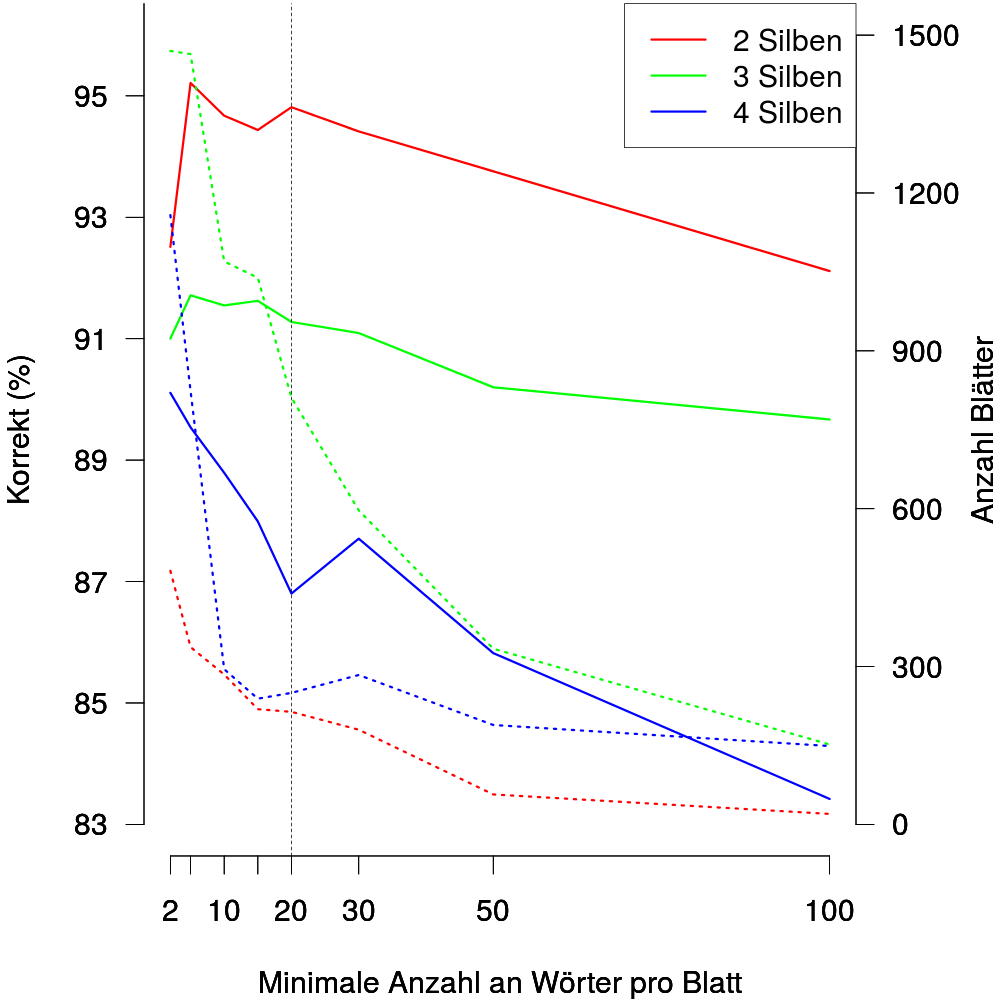
\includegraphics[scale = 0.18]{figures/j48_min_leaves.png}} {
            \label{figure:j48_min_leaves}
            \caption{Einfluss der Anzahl der minimalen Elemente pro Blatt auf die Erkennungsrate (links, fortlaufende Linie) und Breite des Baumes (rechts, gestrichelt). 66\% Training, 33\% Test.}
        }
        \ffigbox{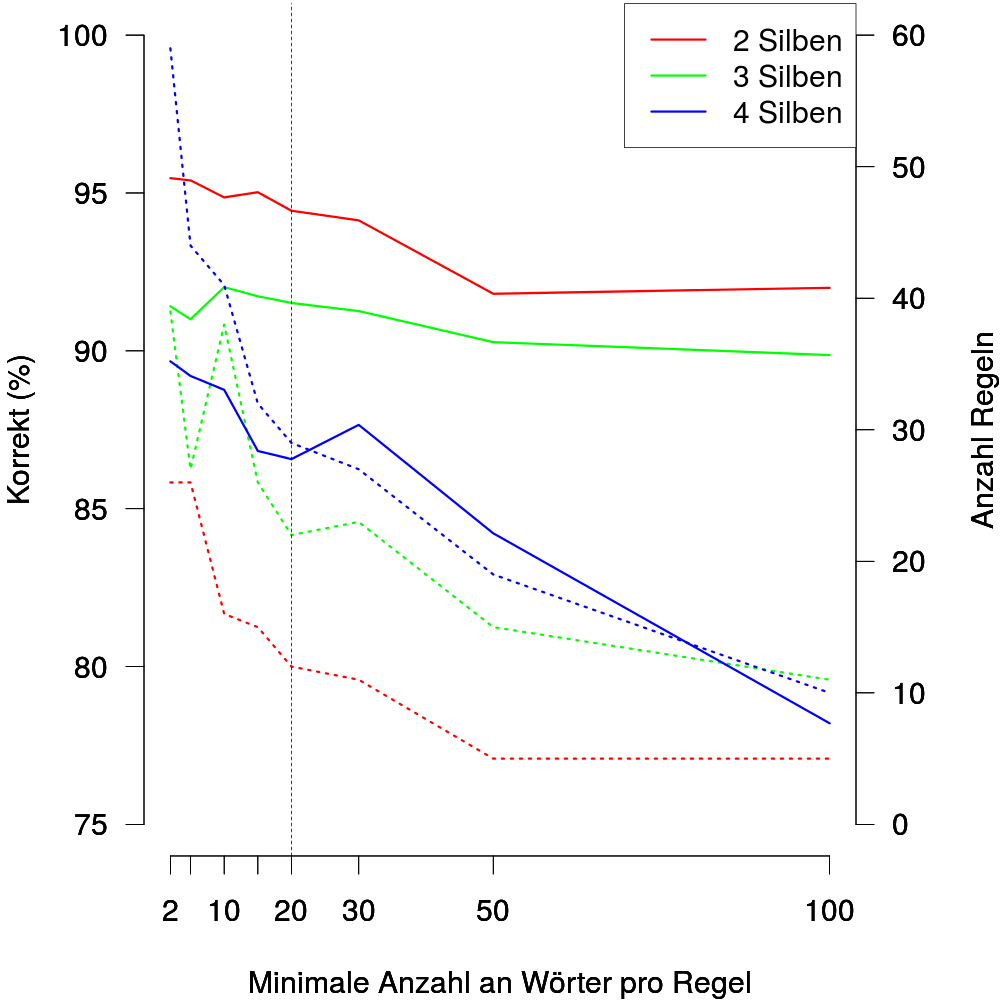
\includegraphics[scale = 0.18]{figures/jrip_min_leaves.png}} {
            \label{figure:jrip_min_leaves}
            \caption{Einfluss der Anzahl der minimalen Elemente pro Regel auf die Erkennungsrate (links, fortlaufende Linie) und Breite des Baumes (rechts, gestrichelt). 66\% Training, 33\% Test.}
        }
    \end{floatrow}
\end{figure}
Beim Training von J48\footnote{Exakte Konfiguration von J48: \texttt{weka.classifiers.trees.J48 -C 0.25 -M 20}} und JRip\footnote{Exakte Konfiguration von JRip: \texttt{weka.classifiers.rules.JRip -F 3 -N 20.0 -O 5 -S 1}} habe ich die minimale Anzahl an Elementen pro Blatt bzw. pro Regel auf 20 limitiert. Durch diese untere Grenze vermeide ich zu spezialisierte Regeln, die nur auf sehr wenige Einzelfälle zutreffen und versuche so irritierendes Rauschen in den Daten auszublenden. Diese Zahl als untere Grenze habe ich empirisch als guten Kompromiss zwischen Kompaktheit und Differenziertheit festgestellt (Abbildung \ref{figure:j48_min_leaves} und \ref{figure:jrip_min_leaves}). Die anderen Parameter habe ich auf ihren Standard-Einstellingen belassen.
Zum Training der Neural Networks habe ich das Modul \textit{NeuralNetwork}\footnote{Verfügbar unter: https://github.com/amten/NeuralNetwork} von Weka verwendet, es bietet Dropout-Regularisierung und RectifiedLinearUnits (ReLUs) als Aktivierungsfunktion. Es ist damit aktuell das modernste und ausgereifteste Neural-Network Modul für Weka. Das Training ist zudem sehr effektiv, kaum eins meiner Modelle hat mehr als 200 Trainingsepochen benötigt, meist reichten ca. 70 Epochen.\\
\begin{figure}[h]
    \centering
    \caption{Ergebnisse der Neuronalen Netze in Abhängigkeit von der Anzahl der Neuronen im Hidden Layer. (66\% Training, 33\% Test)}
    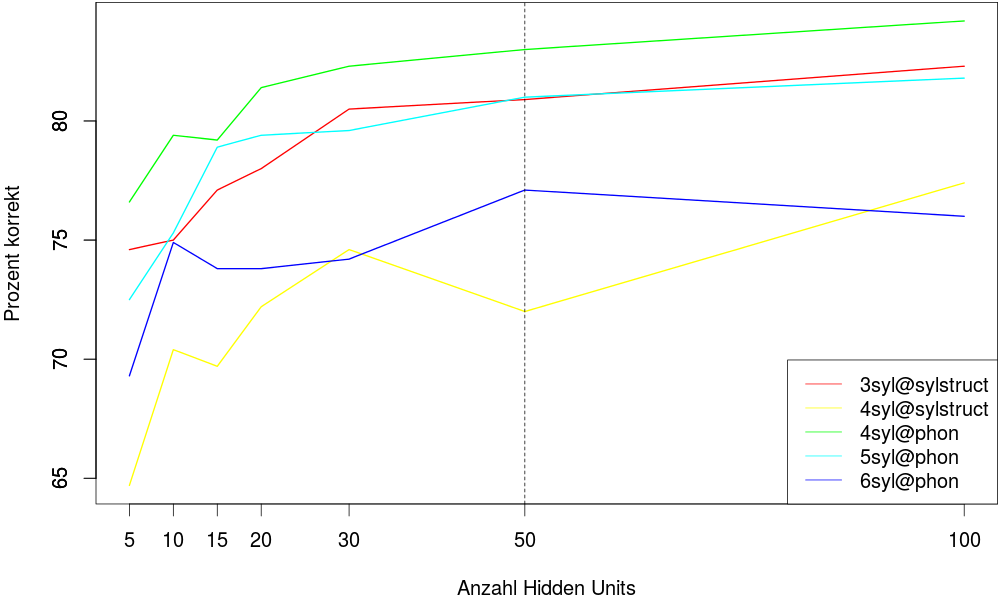
\includegraphics[width=.75\columnwidth]{figures/NN_HUs.png}
    \label{figure:NN_HUs}
\end{figure}
Ich habe eine einschichtige Feed-Forward Architektur mit 50 Hidden Units gewählt\footnote{\label{nn_conf}Exakte Konfiguration des NeuralNetwork: \texttt{weka.classifiers.functions.NeuralNetwork -lr 0.0 -wp 1.0E-8 -mi 1000 -bs 0 -th 4 -hl 50 -di 0.2 -dh 0.5 -iw 0}}. Experimente mit mehr HUs brachten nur geringfügig bessere Ergebnisse (Abbildung \ref{figure:NN_HUs}) und ein weiterer Hidden Layer hat in einzelnen Experimenten auch keine besseren Ergebnisse erzielt. Die längere Trainingszeit und höhere Komplexität des Netzwerks mit mehr Hidden Units wogen für mich schwerer als die geringfügig besseres Ergebnisse. Nach der Regel von \textit{Ockham's razor} sollte man zudem unter gleichwertigen Lösungen die einfachste wählen \cite[S.~652]{RusselNorvig2013}, da Einfachheit an sich eine wünschenswerte Eigenschaft ist, und einfache Modelle besser generalisieren. Obwohl Ockham's razor nicht unumstritten ist \cite{Domingos}, orientiere ich mich in meiner Arbeit an dieser Regel, da einfache Modelle besser verständlich sind und die Gefahr eines Overfittings geringer ist\cite[S.~6]{Domingos}. In meinem Fall bezieht sich Ockham's razor also auf die Architektur des Neural Netowrks mit den wenigsten Neuronen, die Größe des JRip-Regelsets und die Breite des J48-Entscheidungsbaumes.

Als Evaluations-Metrik soll im folgenden die Anzahl an korrekt klassifizierten Wörtern genügen.

\section{Ergebnisse}

Um über die vielen Einzelergebnisse in ihrer Gesamtheit sprechen zu können, ist es notwendig die Ergebnisse sinnvoll zusammenzufassen. Ohne eine entsprechende Aggregation habe ich 6 Datensets (2-7 Silben), 3 Algorithmen (J48, JRip, NeuralNetwork) und 13 Featuresets. Somit gilt es sich einen Überblick über 234 Einzelergebnisse zu verschaffen.

Um die Ergebnisse im Verhältnis zur Schwierigkeit des Problems betrachten zu können stelle ich in jeder Abbildung das Ergebniss des trivialen Baseline-Algorithmus \texttt{ZeroR}, meist als gestrichelte Linie, dar. \texttt{ZeroR} lernt die häufigste Klasse im Trainingsset und klassifiziert alle Wörter des Testsets entsprechend dieser Klasse. Sein Ergebniss stellt somit die \enquote{statistische Nulllinie} dar. Ist ein Algorithmus lediglich so gut wie \texttt{ZeroR}, hat er grob gesagt aus den Features nichts sinnvolles lernen können.

Bei der Betrachtung der folgenden Abbildungen muss man beachten, dass es drei Arten von Featuresets gibt. \texttt{suffix, praefix, sonority, weight, phoncat, meta} sind \textit{grundlegende Featuresets}, die lediglich einen isolierten lingistischen Aspekt betrachten.
Die \textit{kombinierten Featuresets} \texttt{affix} und \texttt{phon} bestehen aus den grundlegenden Featuresets \texttt{praefix} und \texttt{suffix} bzw. \texttt{sonority}, \texttt{weight}, \texttt{phoncat}.
Featureset übergreifende Sammlungen von Einzelfeatures sind die \textit{höheren Featuresets} \texttt{sparse} und \texttt{numeric} während in \texttt{all} sämtliche Features enthalten sind.

Im Folgenden möchte ich zunächst einen Blick auf die Gesamtergebnisse werfen, bei denen die Ergebnisse der einzelnen Modelle nach Trainingssetgröße gewichtet wurden (Abbildung \ref{fig:overall_weighted}). 
% Confusion Matrix => Welche Fehler werden am häufigsten gemacht? Sind seltene Klassen die schwierigen?

\begin{figure}[h]
    \centering
    \caption{Performance je Model, gewichtet über die Trainingssets in Prozent}
    \label{fig:overall_weighted}
    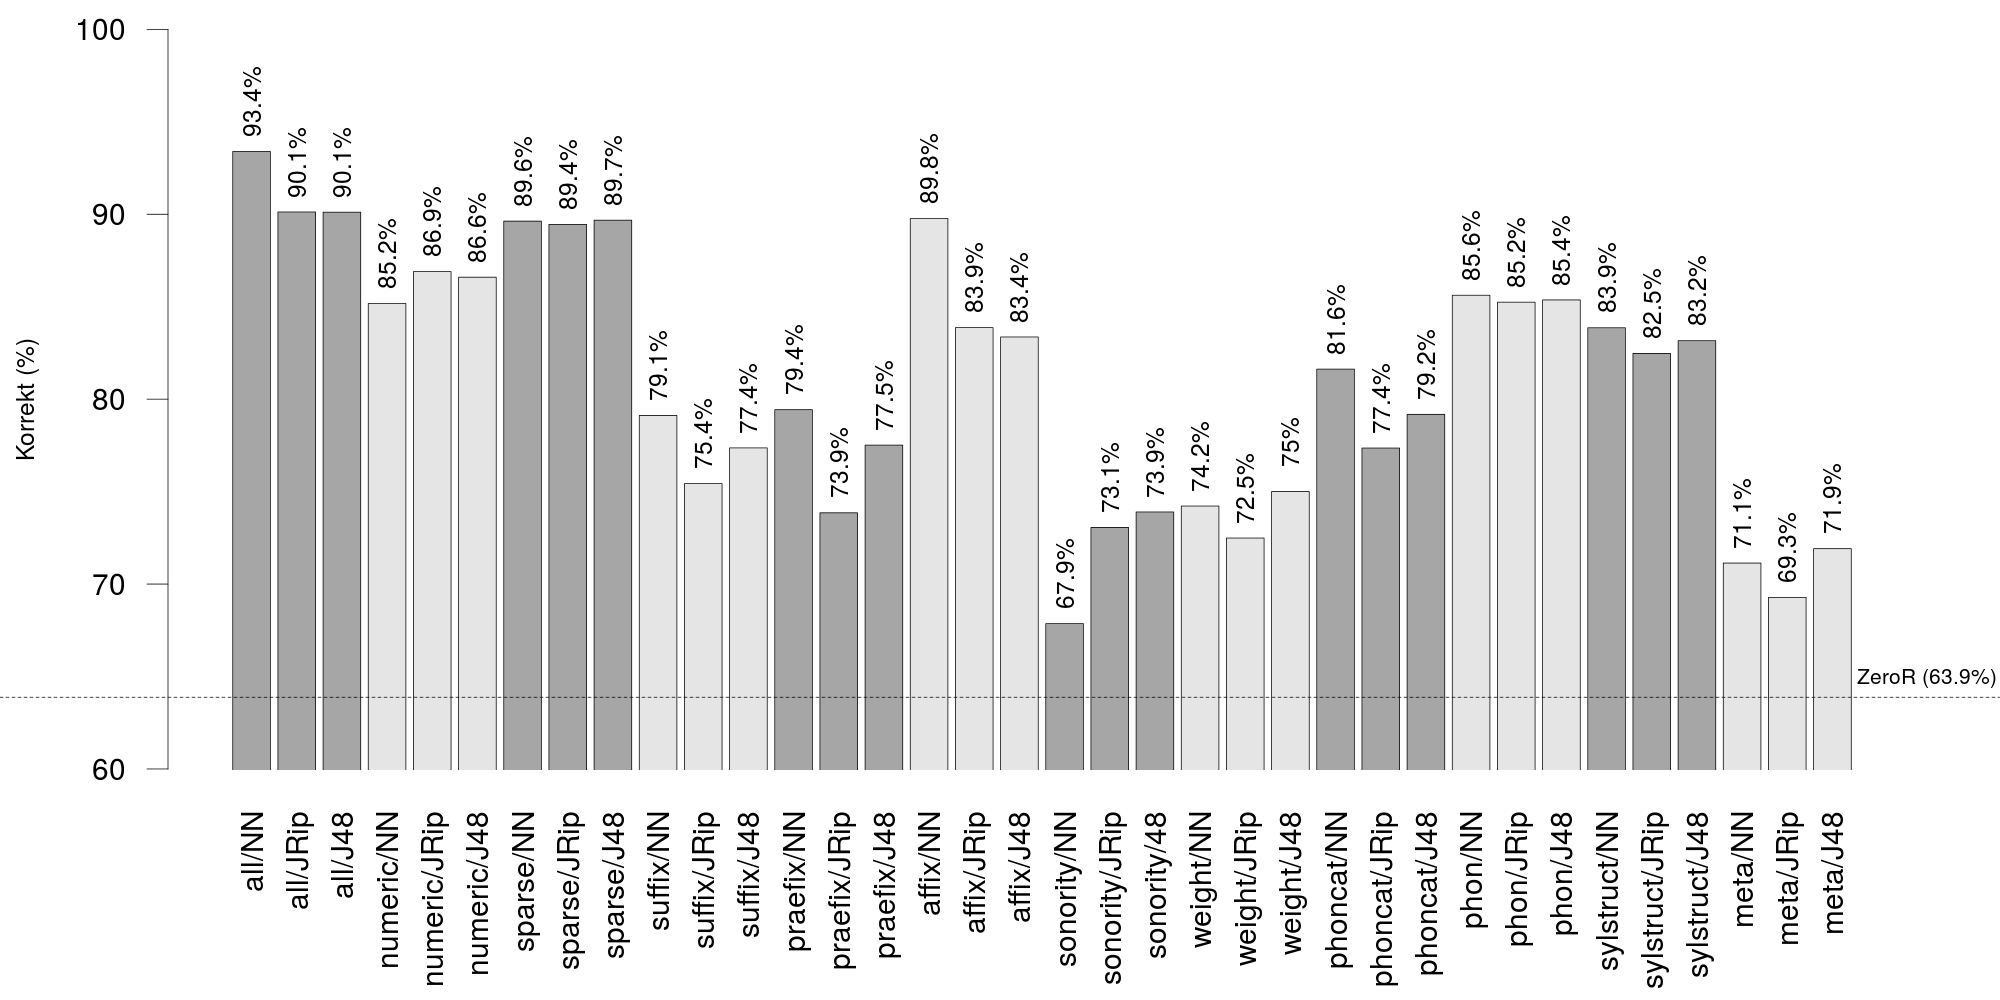
\includegraphics[width=\columnwidth]{figures/esemble/weighted_performance.png}
\end{figure}

Generell kann man der Abbildung \ref{fig:overall_weighted} entnehmen, dass Featuresets mit unterschiedlichen Features besser sind als welche, die nur einzelne linguistische Aspekte betrachten. So sind die Featuresets \texttt{sonority} (67.9-73.9\%), \texttt{weight} (72.5-75.0\%) und \texttt{phonstruct} (77.4-81.6\%) allein eher schwach, in Kombination in \texttt{phon} erreichen alle drei Algorithmen über 85\%. Gleiches trifft auch auf \texttt{praefix} (73.9-79.4\%) und \texttt{suffix} (75.4-79.1\%) sowie ihre Kombination in \texttt{affix} (83.4-89.8\%) zu. Dafür, dass \texttt{sylstruct} ein grundlegendes Featureset ist, erreiche ich mit ihm sehr gute Ergebnisse um die 83\%.  Die drei höheren Featuresets \texttt{all}, \texttt{numeric}, \texttt{sparse} erreichen insgesamt die besten Ergebnisse, angeführt von \texttt{all/NN} mit $93.4\%$. Beste symbolische Modell sind \texttt{all/JRip} und \texttt{all/J48} mit je 90.1\%\\

%Betrachten wir erst die Entscheidungsbäume von J48 hinsichtlich ihrer Varianz. Eine kleine Varianz bedeutet, dass über alle Testsets hinweg ähnliche Erkennungsraten realisiert wurden. Bei kleiner Varianz sind die Features eines Featuresets also unabhängig von der Silbenzahl gleichbedeutend. Sie stellen also Korrelate zum Wortakzent dar, die unabhängig von der Silbenzahl sind, was eine gute Eigenschaft ist. Ist die Varianz groß, ist ein Featureset nicht für alle Silbenanzahlen geeignet, kann jedoch für bestimmten Silbenzahl dennoch gute Ergebnisse liefern. Featuresets mit großer Varianz und guten Ergebnissen sind wahrscheinlich durch Methoden wie Bagging gut anzuwenden.
%Featuresets mit kleiner Varianz und geringen Erkennungsraten sind somit schlecht zur Vorhersage des Akzents geeignet, bei geringer Varianz und hohen Erkennungsraten sind die Features sehr ausdrucksstark. Ist die Varianz groß, werden spezialisiertere Regeln erfasst, die man kombinieren sollte.
%Große Varianz weisen die Affix-Featuresets praefix, suffix und affix auf, ihr Median ist zudem recht gering. Gleiches zeigt sich bei diesem Featuresets bei JRip, insbesondere bei nach unten gibt es starke Ausreißer. Durch die Bediengung, dass jedes Blatt/jede Regel mindestens 20 Elemente enthalten muss fällt es diesen Algorithmen mit abnehmenden Trainingsset-Umfang zunehmend schwerer diese zu berücksichtigen, da die meisten Features dieser Featuresets sehr viele verschiedene Werte enthalten (siehe Tabelle \ref{table:feature_dimensions}). Bemerkenswert sind jedoch die konstant sehr hohen Erkennungsraten von affix/NN. Bei Zwei- bis Viersilbern liefert dieses Modell kurz hinter all/NN die besten Ergebnisse (Detailierte Erkennungsraten siehe Anhang \ref{performance_details}). sonority/NN hingegen ist bei Zweisilbern jedoch nicht besser als ZeroR, wahrscheinlich war die learning rate zu hoch, so dass lediglich die häufigste Klasse gelernt wurde.

\begin{figure}[h]
    \centering
    \caption{Nach Testsetgröße gewichtete Ergebnisse simpler Esembles aus den besten Algorithmen je Feature und Testset. Verbesserung im Vergleich zu Abbildung \ref{fig:overall_weighted} ist grün hervorgehoben.}
    \label{fig:overall_bag}
    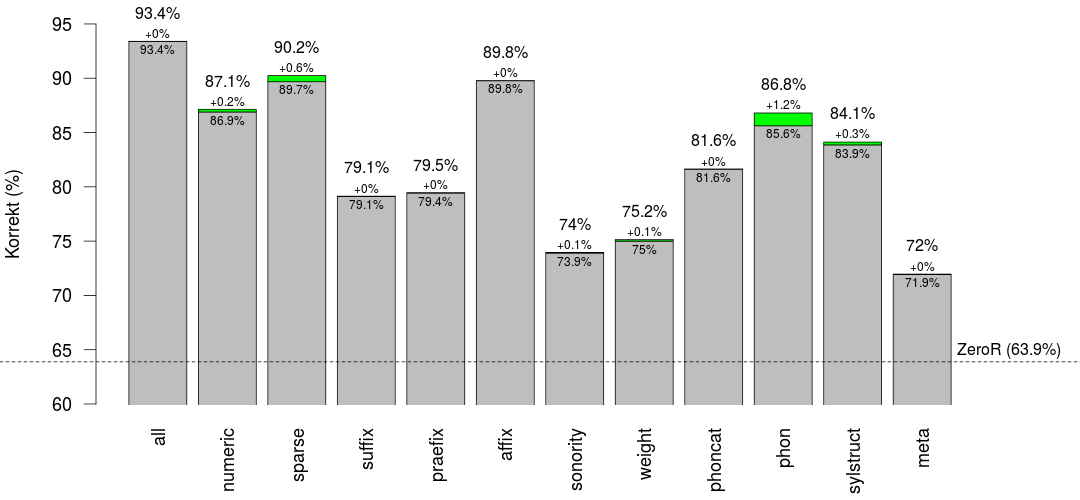
\includegraphics[width=.85\columnwidth]{figures/esemble/bag_of_best_algorithms_for_featuresets.png}
\end{figure}

In Abbildung \ref{fig:overall_bag} sind die Ergebnisse eines simplen Esembles zu sehen, das aus den jeweils besten Modellen der sechs Testsets besteht. Für jedes Testset habe ich je Featureset das beste Modell (J48, JRip oder NN) ausgewählt. Im Falle des phon-Esembles, bestehend aus phon/J48 für Zwei- und Dreisilber und phon/NN für Wörter mit mehr Silben, wird eine Verbesseurng um 1.2\% erreicht. Wahrscheinlich lassen sich die Ergebnisse durch komplexere Esemble-Techniken wie Bagging \cite{Breiman1996} weiter verbessern. Für effektive Anwendung von Esemble-Techniken ist es wichtig, dass die verschiedenen Modelle möglichst wenig korreliert sind, da sie sonst häufiger die gleiche Vermutung für die Klassifizierung abgeben und das Esemble recht sinnlos wäre. Da die Featuresets zum Teil komplett verschiedene linguistische Aspekte betrachten ist anzunehmen, dass sie ausreichend wenig korreliert sind um in Esembles gut verwendet werden zu können. Dies jedoch nur am Rande. Durch Bagging gibt man jedoch die Interpretierbarkeit zugunsten einer höheren Genauigkeit auf \cite[S.\~137]{Breiman1996}, weswegen ich hier diesen Ansatz nicht weiter verfolgen werde.
\newpage

%%
\chapter{Diskussion}
% Der Wortakzents tendiert dazu an den Worträndern zu liegen \textit{demarcative property} \cite[S.~144]{Kager1999}.

%- Welche Ergebnisse wurden erzielt?

%- Welche Einschränkungen wurden gemacht? 

%- Wie verfälschen ggfs. die gemachten Einschränken/Annahmen das Ergebnis?
%- Diskusion der Möglichkeit von Overfitting.

%- Vergleich zu ähnlichen Arbeiten ziehen, Unterschiede evaluieren.

%- Diskussion einiger Theorien der Metrischen Phonologie unter dem Licht dieser Arbeit.

%- Lieber alle Features oder nur eine Auswahl? Mehr Features = Besser?

%- Was sind die Vor- und Nachteile in meinem Anwendungsfall der Algorithmen?
%NN erfasst nichtlinearitäten
%JRip sehr gut interprätier- und auswertbar, jedoch logisch redundant teilweise (length < 3 \&\& length=1)
%J48 sehr schnell, gut zum Experimentieren
\section{Generelles}
\label{generelles}

\begin{figure}[h]
    \centering
    \caption{Erkennungsraten aller Featuresets in Prozent.\\
    Jeder Boxplot enthält die Ergebnisse der Testdaten für 2 bis 7 Silbige Wörter. Die schwarze Linie stellt den Median dar, die maximale Länge der Whiskers beträgt 1.5 IQR.}
    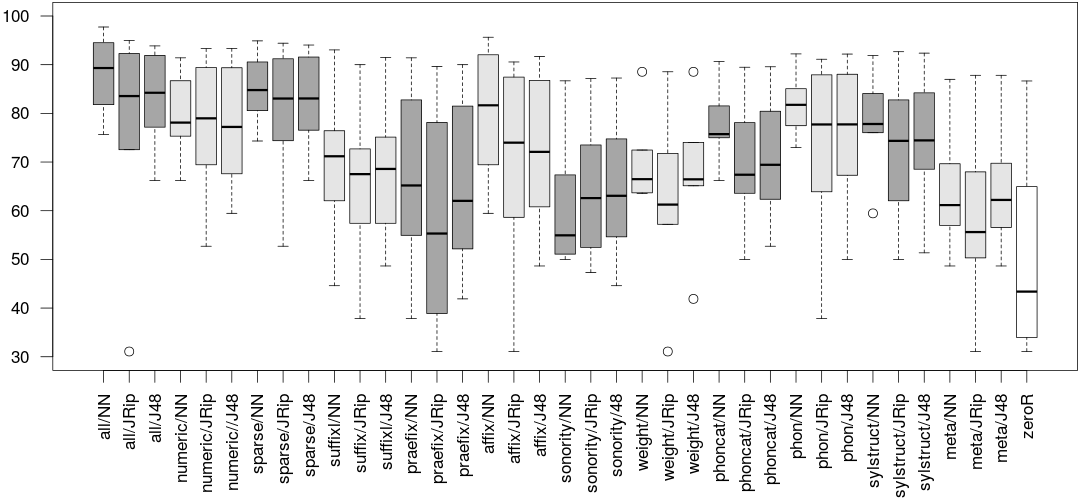
\includegraphics[width=\columnwidth]{figures/featuresets/all.png}
    \label{figure:featuresets_all}
\end{figure}
Die Varianz der Ergebnisse der Featuresets über die Modelle hinweg (Abbildung \ref{figure:featuresets_all}) ist interessant, da eine kleine Varainz eine größere Unabhängigkeit der Regeln von der Silbenanzahl vermuten lässt. Liefert ein Modell über alle Silbenzahlen hinweg ähnliche Ergebnisse, kann man vermuten, dass die Features eine größere Allgemeingültigkeit besitzen bzw. in der Regelhierarchie weiter oben stehen. Das praefix-Featureset besitzt eine sehr große Varianz und teilweise sehr gute Ergebnisse. Die weight-Featuresets erzielen durchweg eher mittelmäßige Ergebnisse, aber dies bei sehr geringer Varianz. Eine Vermutung wäre nun, dass gewisse Praefix-Regeln unter bestimmten Bedingungen andere überschreiben, Regeln des Silbengewichts jedoch deutlich allgemeiner und grundlegender sind. phon/NN und sylstruct/NN besitzen auch beide eine sehr kleine Varianz. Da die Features aus phon sehr nahe der phonetische Repräsentation sind, sind diese sehr Grundlegend.
Die Qualität eines grundlegenden Featuressets kann man auch nach der Invarianz gegenüber der Silbenzahl bei möglichst hoher Abstraktion von der phonetischen Repräsentation beurteilen. Beispielsweise besitzt das phon/NN-Modell eine sehr kleine Varianz und liefert gute Ergebnisse, ist jedoch recht nah der direkten phonetischen Repräsentation. Im Gegensatz dazu besitzen die Modelle des weight-Featuresets zwar keine guten Erkennungsraten, jedoch auch eine sehr kleine Varianz. Das Silbengewicht ist dabei ein sehr abstraktes Maß. Durch dieses Qualitätsmaß lassen sich somit Hinweise finden, wie gut linguistische Konzepte verallgemeinerbar sind. In diesem Kontext scheinen praefix und sonority für sich genommen keine gutes Konzepte zu sein.
Wie wir später sehen werden, sind jedoch grade diese beiden Features in Kombination mit anderen sehr gute Regeln möglich. Als einziges Qualitätsmaß ist die Invarianz gegenüber der Silbenzahl daher wohl nicht ausreichend.


\subsection{Die Ergebnisse im Kontext der Korpusgröße und Schwierigkeit der Klassifikation}
\begin{figure}[hb]
    \centering
    \caption{Erkennungsrate je Testset. Differenz der besten Modelle (dunkelgrau) zu ZeroR (hellgrau). Die Breite der Barplots ist proportional zur Anzahl der enthaltenen Wörter.}
    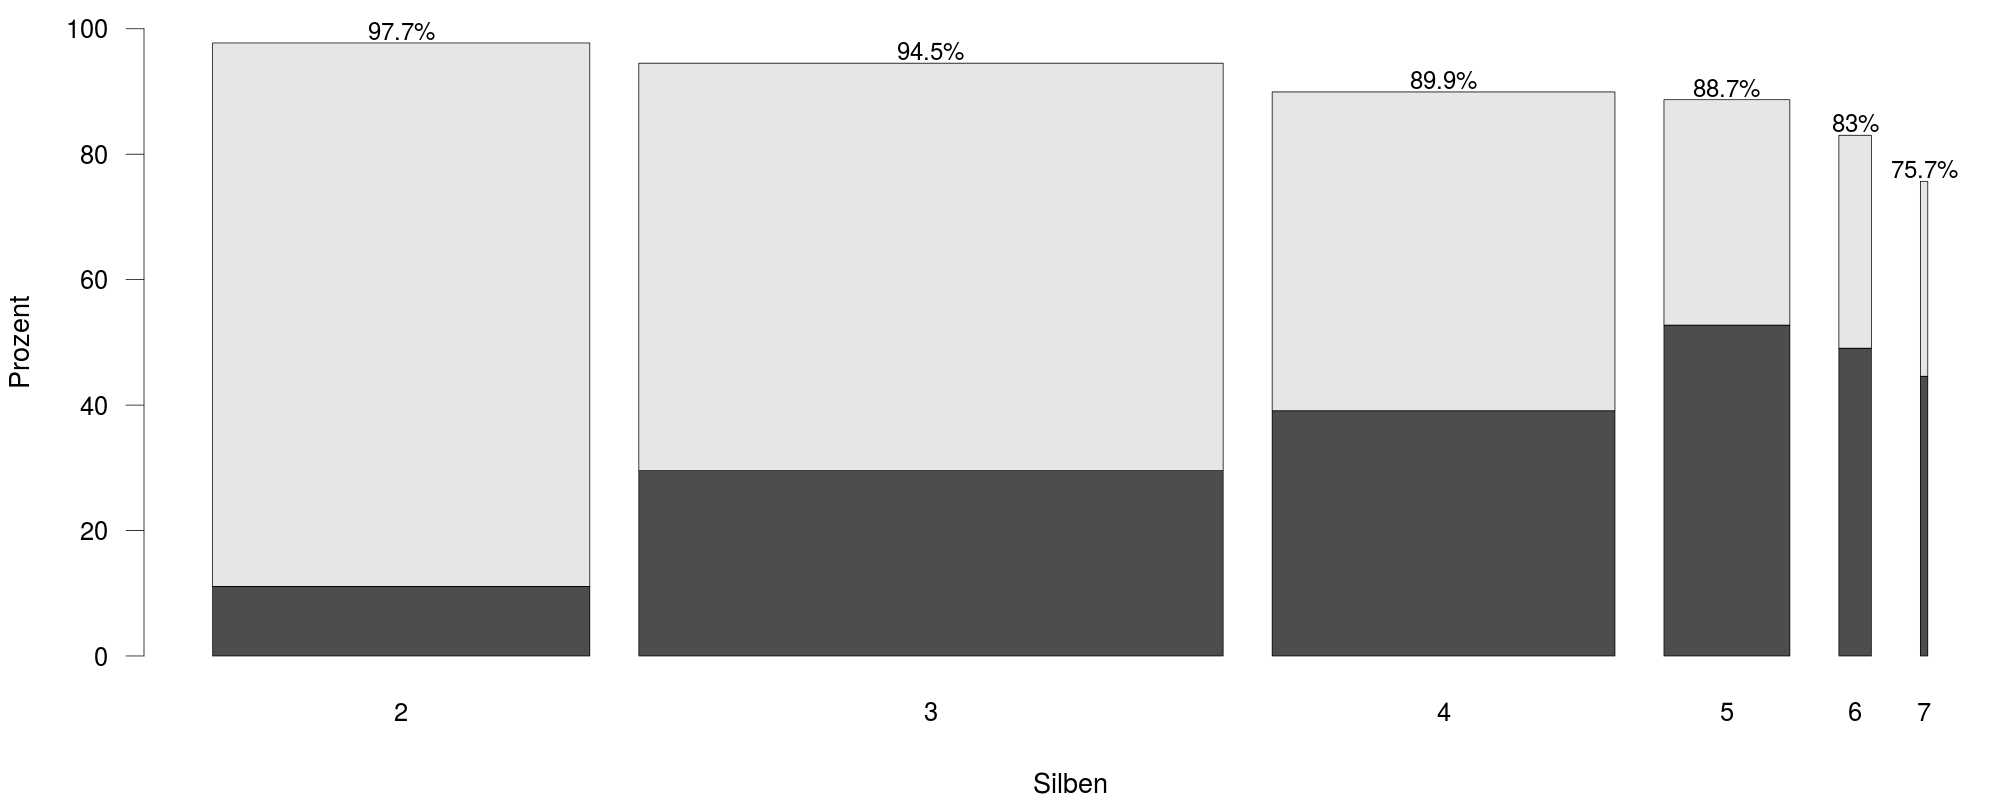
\includegraphics[width=.75\columnwidth]{figures/performance_by_syllables.png}
    \label{figure:results_proportional}
\end{figure}

Wie gut sind meine Ergebnisse wirklich? In Abbildung \ref{figure:results_proportional} sieht man die Differenz des besten Ergebnisses zu ZeroR. Man sieht die positiven Einflüsse der größeren Trainingsmenge sowie das mit zunehmender Silbenanzahl schwieriger werdende Klassifizierungsproblem. Bis fünf Silben wird mit jeder weiteren Silbe ZeroR um etwa ein Viertel schlechter. Sobald alle fünf möglichen Betonungsklassen tatsächlich möglich sind, also die Wörter fünf oder mehr Silben besitzen, liegt ZeroR mehr oder minder konstant bei 30-35\% (siehe Anhang \ref{performance_details}).

\begin{table}[h]
\centering
\caption{Anzahl an Wörter je Trainingsset mit von der häufigsten Klasse abweichender Betonung (gerundet).}
\label{table:wertvolle_woerter}
\begin{tabular}{|ccc|}\hline
{\bf Silben} & {\bf \enquote{wertvolle} Wörter} & {\bf Prozent} \\\hline
2            & 1000                     & 13.3\%   \\
3            & 4000                     & 34.3\%   \\
4            & 3400                     & 49,7\%   \\
5            & 1600                     & 63.7\%   \\
6            & 400                      & 61.2\%   \\
7            & 100                      & 67.6\%   \\\hline
\end{tabular}
\end{table}
Anders gesehen gibt die dunkelgraue Fläche die Anzahl an Wörtern an, die von der häufigsten Klasse abweichen, die also einen höheren Informationsgehalt haben, als die der häufigsten Klasse. So gibt es bei Drei- und Viersilbern die meisten wertvollen Worte, rund viermal so viele wie bei den Zweisilbern (Tabelle \ref{table:wertvolle_woerter}). In diesem Licht ist das Ergebnis der Zweisilber von 97.4\% wahrscheinlich nicht so gut wie es mit den gegebenen Features sein könnte. Mit zunehmender Silbenzahl wird zwar die Klassifizierung schiweriger, jedoch ist der Umfang der Trainingsdaten auch höher, so dass Drei-, Vier- und Fünfsilber trotz des jeweils 1/4 schweren Problems nur geringfügig schlechter sind. Insbesondere bei Fünfsilbern merkt man den Wert von Wörtern mit hohen Informationsgehalt. Obwohl die Gesamtgröße des Trainingssets der Fünfsilber nur ein Drittel so groß ist wie das der Zweisilber, enthält es 40\% mehr wertvolle Wörter. Obwohl das Klassifizierungsproblem doppelt so schwierig ist wie bei Zweisilbern, erreiche ich auf den Fünfsilbern ein nur 9\% schlechteres Ergebnis. Bei den Sechs- und Siebensilbern erkennt man die Auswirkungen der zu kleinen Trainingssets, die Ergebnisse werden verglichen mit den Fünsilbern deutlich schlechter, obwohl das Klassifizierungsproblem etwa gleich schwierig bleibt. Versuchsweise habe ich die Trainings- und Testsets der Fünfsilber dem Umfang der Sechssilber angepasst, um zu sehen, ob man die Beobachtung reproduzieren kann. Tatsächlich erhalte ich statt 88.7\% auf \texttt{all/NN} nun 82.6\% - auf Sechssilbern waren es 83\%. Daraus schlussfolgere ich, dass bei Wörtern mit 5-7 Silben die Lernkurve sehr ähnlich ist.

\subsection{Ergebnisunterschiede auf den \texttt{affix}-Modellen}

Besonderes Augenmerk verdienen die Ergebnisse der \texttt{affix}-Modelle. \texttt{affix/NN} erreicht 89.7\%, während das selbe Featureset in Kombination mit JRip und J48 über 6\% schlechter ist. Woher rührt dieser große Unterschied? Wahrscheinlich kommt er daher, dass jede Regel/jedes Blatt mindestens 20 Wörter enthalten muss. Solch eine Einschränkung gibt es bei den Neuronalen Netzen nicht, sodass jeder noch so seltene Wert eines Feature berücksicht werden kann. Aber lernt das NN nicht einfach nur die Worte auswendig? Immerhin werden unter anderem die führenden und die letzten fünf Phoneme direkt als Features übergeben. Heißt dass, alle Wörter mit weniger als 11 Phonemen werden direkt dem NN übergeben, meist also das gesamte Wort? Nein, denn seltene Werte werden aus den Features gelöscht, so dass ausschließlch die 20 bis 100 häufigsten als Features verwendet werden (Details siehe Anhang \ref{attr_counts}). So ist es möglich häufige Wortanfänge/-enden genau zu differenzieren, und seltenere durch ein Feature mit höherem Abstraktionsgrad (\texttt{prae-/suffix\_phoncat}) auch mit zu erfassen. Da die Wortbetonungen neigt an den Worträndern zu liegen, reicht es offensichtlich beinahe aus, ausschließlich diese bei der Akzentzuweisung zu betrachten. Vielleicht lernen die NN jedoch auch gewisse nichtlineare Korrelationen zwischen Affixen, die den beiden linearen Lernverfahren natürlich verborgen bleiben. Nichts desto trotz haben sich die Affixe als aussagekräftigstes Featureset herausgestellt, von den drei höheren Featuresets abgesehen. Durch Einbeziehung aller weiteren verfügbarer Features in \texttt{all/NN} wird das Ergebnis lediglich um 3.6\% verbessert.

\subsection{Mehr Features, bessere Ergebnisse?}
\label{features_performance_dependancy}
\begin{figure}[h]
    \centering
    \caption{Ergebnisse der Modelle im Verhältnis zur Größe des Featuresets. Bestes Modell je Testset ist hervorgehoben.}
    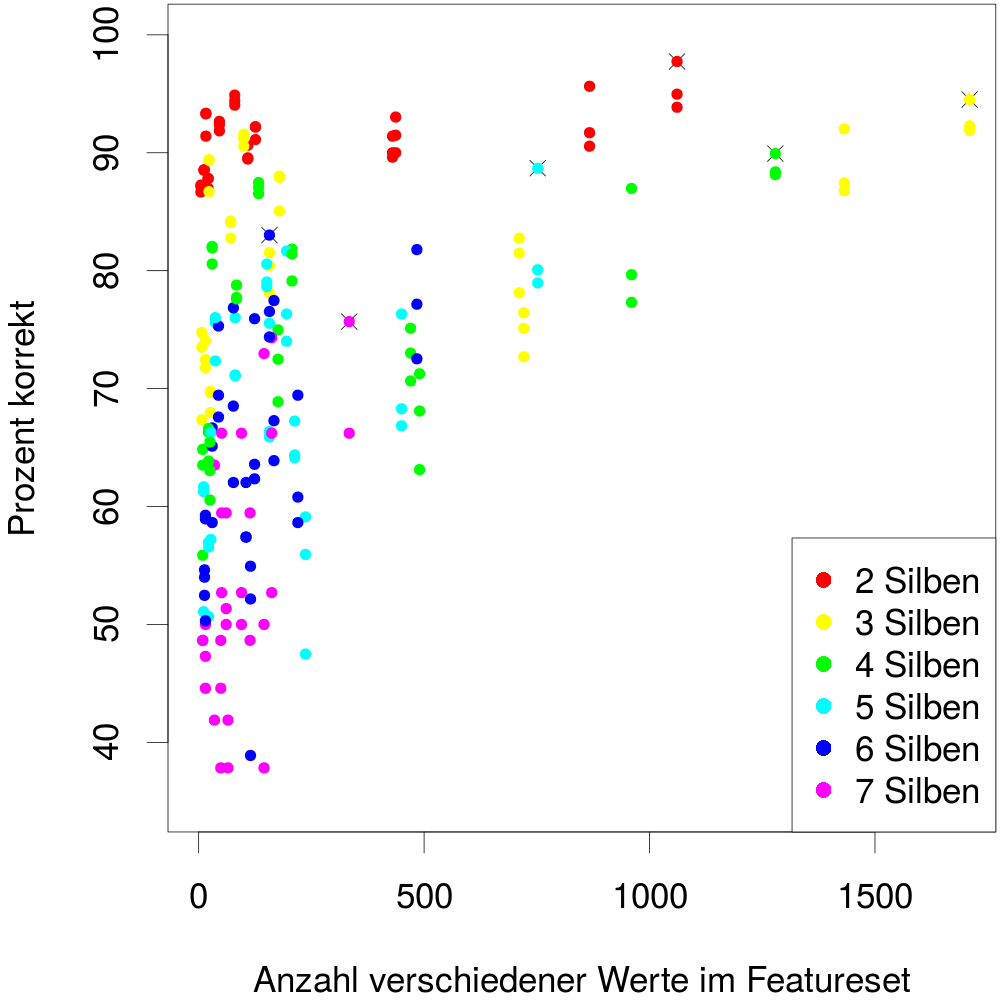
\includegraphics[width=.5\columnwidth]{figures/counts_vs_performance.png}
    \label{figure:counts_vs_performance}
\end{figure}
Den Begriff \enquote{Features} habe ich in der bisherigen Arbeit als \textit{Sammlung} von Merkmalen verwendet. So ist ein beispielsweise \enquote{Hat Suffix \textit{-en}?} ein  Merkmal und \enquote{Hat Suffix \textit{-heit}} ein weiteres. Beide subsumiere ich unter dem Feature \texttt{suffix}, obwohl es eigentlich viele verschiedene Flags sind, ob ein Merkmal vorhanden ist. Wenn ich im Folgenden über die \textit{Merkmalsanzahl} von Feature(sets) spreche, meine ich damit die Gesamtanzahl an Flags für Merkmale von Features. Diese Zahl entspricht im Übrigen der Zahl der Input-Neuronen in Neuronalen Netzen. Numerische Werte zählen ich dabei als ein Wert, da meinen symbolischen Lernverfahren lediglich größer und kleiner unterscheiden und in NN dafür lediglich ein Neuron benötigt wird. Die genaue Zahl der Merkmale je Feature, Featureset und Silbenzahl findet sich in Anhang \ref{attr_counts}

Bis auf eine Ausnahme sind für alle Testsets die Topergebnisse mit dem Featureset erreicht worden, dass die größte Merkmalsanzahl hat (Anhang \ref{performance_details}). Ist es möglich, dass durch die teils sehr große Anzahl an Merkmalen so viele kleine Korrelationen aufsummiert wurden, bis ein gutes Ergebnis erzielt wird? So würde zwar das Modell unter Umständen gut generalisieren, hätte jedoch lediglich statistische Kleinigkeiten zu einem Großen zusammengefügt. Somit wäre man weit von den Kausalzusammenhängen entfernt und tut im Kern dasselbe wie n-Gramm Modelle u.ä. in vergangenen Arbeiten.

Abbildung \ref{figure:counts_vs_performance} scheint gegen diese Vermutung zu sprechen. Mit der Zahl der Merkmale steigt zwar sehr verlässlich die Zahl der richtig klassifizierten Wörter, jedoch lediglich als untere Schranke. Nach oben hin ist kaum ein Zusammenhang zwischen Merkmalsanzahl und Erkennungsrate festzustellen. Gute Ergebnisse mit 100 Merkmalen liegen nur wenige Prozentpunkte vom Topergebnis mit über 17x mehr Merkmalen entfernt, um die Dreisilber als Beispiel zu verwenden (Details siehe Anhang \ref{performance_details}). So ist anzunehmen, dass in meinen Features es einige wenige, wirklich ausdrucksstarke Merkmale gibt und die Ergebnisse der Featuresets mit deutlich mehr Merkmalen lediglich zusätzlich noch viele schwache Korrelationen ausnutzen.

Unter dem Aspekt der (linguistischen) Wissensgewinnung ist es also sinnvoll nicht die besten Modelle zu analysieren, sondern diejenigen, die mit möglichst wenig Feautres noch gute Ergebnisse erzielen.

\subsection{Evaluation der Algorithmen}
% Gibt es Unterschiede innerhalb der Performance der Algorithmen untereinander? Falls ja, woher rühren diese?
Im vorherigen Abschnitt \ref{features_performance_dependancy} habe ich hervorgehoben, dass Featuresets mit wenigen Merkmalen besser zur linguistischen Analyse geeignet sind, auch wenn sie nicht die besten Ergebnisse liefern. Gleiches gilt für die generierten (symbolischen) Wissensrepräsentationen, also die Regelsets und Entscheidungsbäume. Abbildungen \ref{figure:algorithms_J48} und \ref{figure:algorithms_JRip} stellt die Komplexität der Wissensrepräsentationen mithilfe verschiedener von mir gewählten Metriken dar. Sind bei den Featuresets möglichst offensichtlich weniger Merkmale wünschenswert, gestaltet sich die Sache nun etwas diffizieler. Der Idealfall ist ein Modell mit wenigen kurzen Regeln. Ein Modell mit vielen, aber dafür kurzen Regeln sowie eines mit wenigen, jedoch langen Regeln kann dennoch auch wünschenswert sein. In jedem Fall sollten viele und dabei lange Regeln vermieden werden. 

In einem Entscheidungsbaum stellt jeder Pfad von der Wurzel zum Blatt eine Regel dar, verbunden durch Konjunktionen, die Länge des Pfades entspricht der Tiefe des Blattes. Die Tiefe eines Blattes entspricht also der Anzahl der Komponenten der Konjunktion und damit der Länge der Regel. Eine Regel der Länge drei besitzt somit drei \enquote{und}'s und vier Vergleiche wie z.B. \texttt{sonority2 > 10}. Die Blattiefe bei J48 entspricht also der Regellänge bei JRip und die Anzahl der Blätter ist J48's Pedant zur Anzahl der JRip-Regeln. 

\begin{figure}[h]
    \begin{floatrow}
        \ffigbox{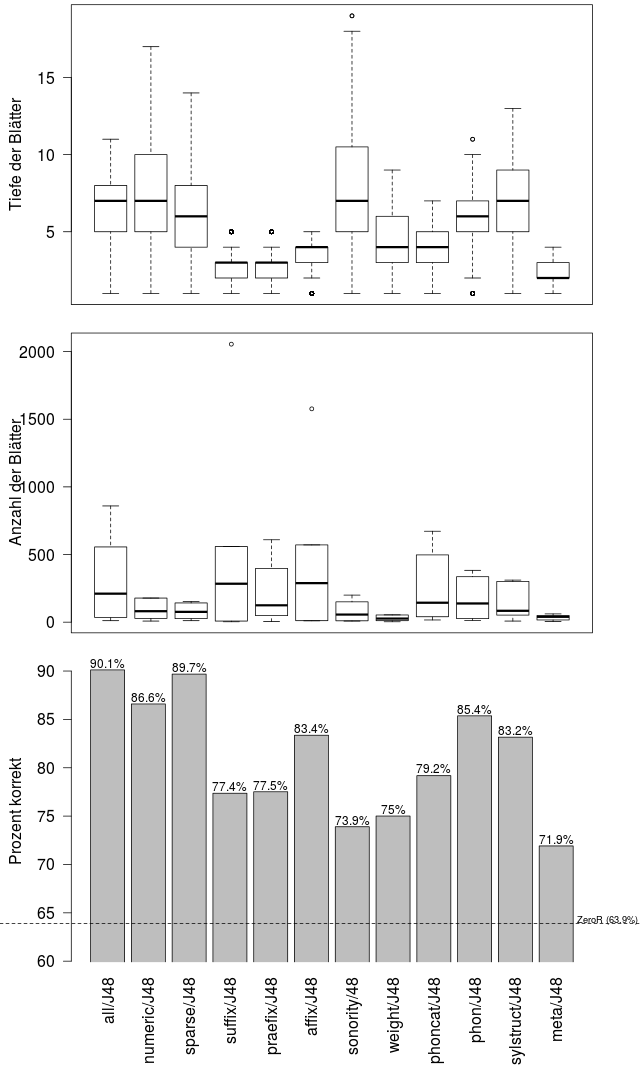
\includegraphics[scale = 0.3]{figures/algorithms/J48.png}} {
            \caption{Metriken zur Analyse der Entscheidungsbäume. Die Tiefe entspricht der Länge der Regel und die Anzahl der Blätter der Anzahl der JRip-Regeln.}
            \label{figure:algorithms_J48}
        }
        \ffigbox{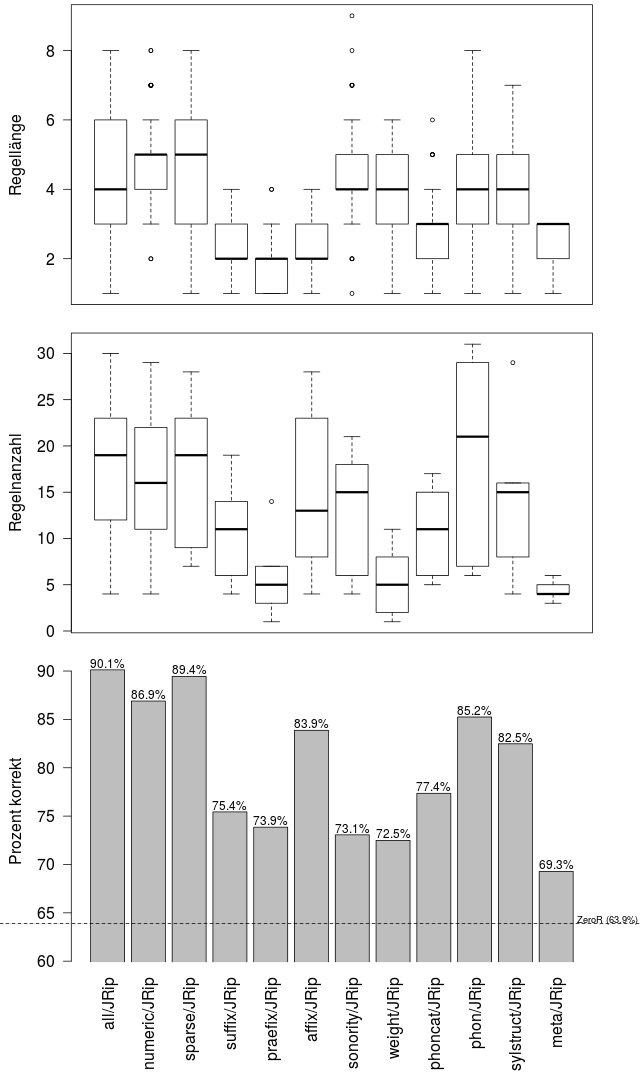
\includegraphics[scale = 0.3]{figures/algorithms/JRip.png}} {
            \caption{Metriken von Analyse der JRip-Regelsätze}
            \label{figure:algorithms_JRip}
        }
    \end{floatrow}
\end{figure}

Ab wann eine Regel \enquote{zu lang} oder ein Regelset \enquote{zu groß} ist, kann man nicht pauschal sagen. Die Anzahl der Regeln wiegt dabei in meinen Augen schwerer als die Länge der Regeln. Die Größe der JRip-Regelsets ist dabei stehts sehr überschaubar, keins hat mehr als etwa 30 Regeln. Die Bäume von J48 hingegen haben oft eine Breite von 500 oder mehr, auch wenn die Mediane um 100-200 herum liegen.
Bei J48 hat das all-Featureset als einziges Modell sowohl eine große Anzahl Blätter als auch gleichzeitig eine recht große Blatttiefe. numeric, sparse, sonority und sylstruct haben zwar sehr Tiefe Blätter, dafür aber nur sehr wenige Knoten. Sie haben jedoch mit die kleinste Merkmalsanzahl (Anhang \ref{attr_counts}), weswegen es nicht verwunderlich ist, dass der Baum statt in die Breite in Tiefe gewachsen ist.
suffix und affix haben beide zwei Ausreißer nach oben in der Anzahl der Blätter. Sie sind neben all und praefix die Featuresets mit den meisten Merkmalen. Diese lassen sich durch die Art und Weise erklären, wie der Baum konstruiert wird. Entscheidet sich beispielsweise der Algorithmus dafür, nach suffix3 zu Unterscheiden, \textit{müssen} alle Werte etwa 90 Ausprägungen (=verschiedene Merkmale) des Features berücksichtigt werden. Geschieht das mehrfach in Folge exponentiert sich die Anzahl der Blätter sehr schnell.

Welche Featuresets sind nun zu bevorzugen bei der Analyse? Das Modell \texttt{all/J48} erzielt zwar die besten Ergebnisse, besitzt jedoch als einziges in Abbildung \ref{figure:algorithms_J48} eine recht große Tiefe und dabei sehr viele Blätter. Es besitzt also beide, eben beschriebenen, nicht wünschenswerte Eigenschaften. Hingegen besitzt sparse/J48 recht wenig Blätter, die zwar recht Tief sind, dafür aber auch das zweitbeste Ergebnis liefert. phon sieht des weiteren vielversprechend aus, Tiefe und Anzahl der Blätter sind in Ordnung, ebenso wie seine Ergebnisse.
Auch hier sticht sonority wieder negativ heraus. Es hat die tiefsten Blätter und das zweitschlechteste Ergebnis, jedoch recht wenige Blätter. Allein scheint dieses Feature sehr schlecht geeignet, den Wortakzent vorherzusagen.  

Bei JRip ist das Problem, dass die Featuresets mit wenigen, kurzen Regeln allesamt schlechte Ergebnisse liefern. Lediglich sieht affix hat sehr kurze Regeln, wenn auch recht viele. Es ist dennoch unter den höheren Featuressets von den Ergebnissen her das schlechteste. Besonders schlecht schneidet wieder sonority mit schlechten Ergebnissen und vielen, langen Regeln ab. Da die Anzahl der Regeln jedoch trotz einer gewissen Varianz stets sehr gering ist, sollte dies kein Argument sein, sie nicht zu untersuchen. Auch die Länge der Regeln ist nicht allzu groß, weswegen es vielversprechend erschient, die mit den besten Erekkungsraten weiter zu untersuchen.

Problematisch bei meinen Metriken ist jedoch, dass der Einfluss der Regeln nicht berücksichtigt wird. So ist es möglich und wahrscheinlich, dass unter vielen langen Regeln auch eine kurze dabei ist, die sehr viele Wörter mit hoher Genauigkeit klassifiziert.
Kritik der Metriken: Einfluss der Regeln nicht berücksichtigt. Viel Totholz, dass den Baum aufbläßt.

%Die Entscheidungsbäume besitzen bei mir eine maximale Tiefe von 10-15, teils bis fast 20, und eine Breite (Anzahl der Blätter) von bis zu 500. Die JRip-Regeln hingegen sind nie länger als 9 Komponenten, meist noch deutlich kürzer, und kein Regelset enthält mehr als ca. 30 Regeln.\\
%So betrachtet sind die JRip-Regeln um ein vielfaches ausdrucksstärker und genereller als die weit ausladenden Entscheidungsbäume von J48. Bei einer Reduktion der Regelanzahl um ca. Faktor 10 sind die Ergebnisse von JRip meist kaum schlechter, in zwei Fällen sogar besser als von J48.

\subsection{Evaluation der Features}

\subsubsection{Manuelle Analyse der Regeln}
Bei der manuellen Durchsicht der Regeln (Auswahl in Anhang \ref{table:jrip_rules_examples}) fallen einige interessante Dinge auf. Recht häufig gibt es im selben Regelset mehrere Regeln, die sich lediglich in einer, oder einigen wenigen, Komponente unterscheiden. Jede Regel dieser \enquote{Regelfamilie} ist für sich genommen recht gut, jedoch ist die Schnittmenge der Wörter, die unter diese Regeln fallen groß. Die Regeln in Abbildung \ref{figure:jrip_tree} klassifizieren zusammen also nicht 1271 Wörter richtig, sondern deutlich weniger.

\begin{figure}
    \tiny
    \centering
    \Tree   [.{comp\_len $\leq$ 1}
                [.{nucleus\_phoncat2 = L}
                    [.{onset\_len0 $\geq$ 1}
                        {pos = V\\\textit{328/8}}
                        {syl\_suffix = ren\\\textit{321/2}}
                        [.{syl\_weight1 = light}
                            [.{prae\_class = ø}
                                {onset\_phoncat3 = C\\\textit{224/40}}
                                [.{syl\_open1 = o}
                                    {sonority\_ratio3 $\leq$ 4\\\textit{34/3}}
                                ]
                            ]
                            {suffix\_phoncat4 = LCKC\\\textit{154.0/27.0}}
                        ] !\qsetw{3cm}
                    ]  !\qsetw{4cm}
                    [.{cv\_ratio1 $\leq$ 0}
                        {syl\_len3 $\geq$ 4\\\textit{167/13}}
                    ]
                    {\qsetw{1cm}suffix3 = sch\\\textit{43/16}}
                ]
            ]
    \caption{Aus sieben ähnlichen JRip-Regeln verschiedener Featuresets generierter Entscheidungsbaum für Viersilbern.\\Die Zahlen unter den Blättern sind die Anzahl an True Positives bzw False Positives. Jeder Ast verbindet zwei Knoten mit einem \enquote{und}.}
    \label{figure:jrip_tree}
    \normalsize
\end{figure}
Eine weiterer Punkt ist, dass viele Regeln unnötig kompliziert sind und teilweise redundant sind. Oft findet man Konstrukte wie \texttt{sonority1 $\geq$ 11 and sonority1 < 11} in den Regeln, da numerische Werte bei JRip nur durch Ungleichungen verglichen werden. Ein weiteres Beispiel ist die Regel \texttt{nucleus\_phoncat0 = K and syl\_phoncat0 = CK}. Ist die Silbe der Gestalt Konsonant (C) - Kurzvokal (K), so ist trivialerweise der Nucleus ein Kurzvokal, da Vokale immer den Nucleus bilden. Extrem häufig beziehen sich Regeln nur auf Nonkomposita (\texttt{comp\_len <= 1}), was für den Linguisten auch wenig interessant ist, da die Betonung von Komposita eigenen Regeln folgen. In sehr vielen Fällen kann man somit noch eine Komponente der Regeln streichen.\\
Mit ein wenig Hintergrundwissen lassen sich die Regeln teils stark vereinfachn. Ein Beispiel ist die Regel \texttt{(nucleus\_phoncat0 = K) and (syl\_weight1 = light) and (sonority0 \textless= 11) and (sonority0 \textgreater= 10) and (syl\_phoncat0 = CKC) and (sonority0 \textgreater= 11)}, die sich mit ein wenig Nachdenken wie folgt schreiben lässt: \texttt{(syl\_phoncat0 = CKC) and sonority0=11 and (syl\_weight1 = light)}. Zudem ergibt sich aus einem Blick in die Tabellen \ref{table:sonority} und \ref{table:phoncats}, dass in einer Silbe der Form CKC eine Sonorität von 11 nur mit bestimmten Klasse von Phonemen möglich ist: Liquid (Sonorität 4) - Approximant (Sonorität 6) - Plosiv/Affrikat/Frikativ (Sonorität 1) bzw. Anfang und Ende vertauscht. Diese anfänglich recht kompliziert erschienende Regel trifft auf ca. 1000 Dreisilber des Testsets zu und klassifiziert rund 80\% davon richtig als paenultimabetont.\\
Vielleicht findet sich diese Regel auch in Regelsets für Wörter mit anderen Silbenzahlen wieder? Woher rühren die 20\% falsch klassifizierten Wörter dieser Regel? Ist die Einteilung der Phonemklassen oder die Sonoritätsskala schuld? Gibt es ähnliche Regeln, die Hinweise zum eigentlichem Kausalzusammenhang liefern können? Da der Zweck dieser Arbeit nicht die Klärung dieser linguistischen Fragen ist, belasse ich es bei diesem Beispiel, das demonstriert welch mächtiges Hilfsmittel die hier angewandten Verfahren sind. In der manuellen Durchsicht der Regeln finden sich noch Unmengen an weiteren Zusammenhängen und Gesetzmäßigkeiten. Es ist jedoch ersichtlich, dass ein gewisses, teils recht umfangreiches Hintergrundwissen notwendig ist, um aus den automatisch generierten Regeln neue Schlüsse ziehen zu können. Maschinelle Verfahren können dabei helfen den Fokus auf die richtigen Aspekte zu lengen, das Schlüsse ziehen nehmen sie uns leider jedoch nicht komplett ab.
\label{rule_simplify}


%%%%%%%%%%%%

%Durch die trennung der Wörter entsprechend ihrer Silbenzahl kann man außerdem beobachten, wie Regeln, die für Wörter mit wenig Silben sehr gut sind, mit steigender Silbenanzahl schlechter werden, man könnte es verrauscht oder gestört nennen. Dies spricht für die Theorie von hierarchischen Regeln, die sich gegenseitig überfahren können.  


%\begin{wraptable}{r}{5cm}
%\centering
%\small
%\caption{Ausdrucksstärkste JRip-Regel bei Dreisilbern:\\(prae\_class = noacc) \\$\implies$ Sekunda wird betont}
%\label{table:noacc_sekunda}
%\begin{tabular}{|cc|}\hline
%{\bf Silben} & {\bf TP/FP}    \\\hline
%2            & 76/0           \\
%3            & 1560/1         \\
%4            & 392/2          \\
%5            & $\approx 98/6$ \\
%6            & 41/5           \\
%7            & -              \\\hline
%\end{tabular}
%\end{wraptable} 

\subsubsection{Einfluss der Features}

\begin{figure}[h]
    \begin{floatrow}
        \ffigbox{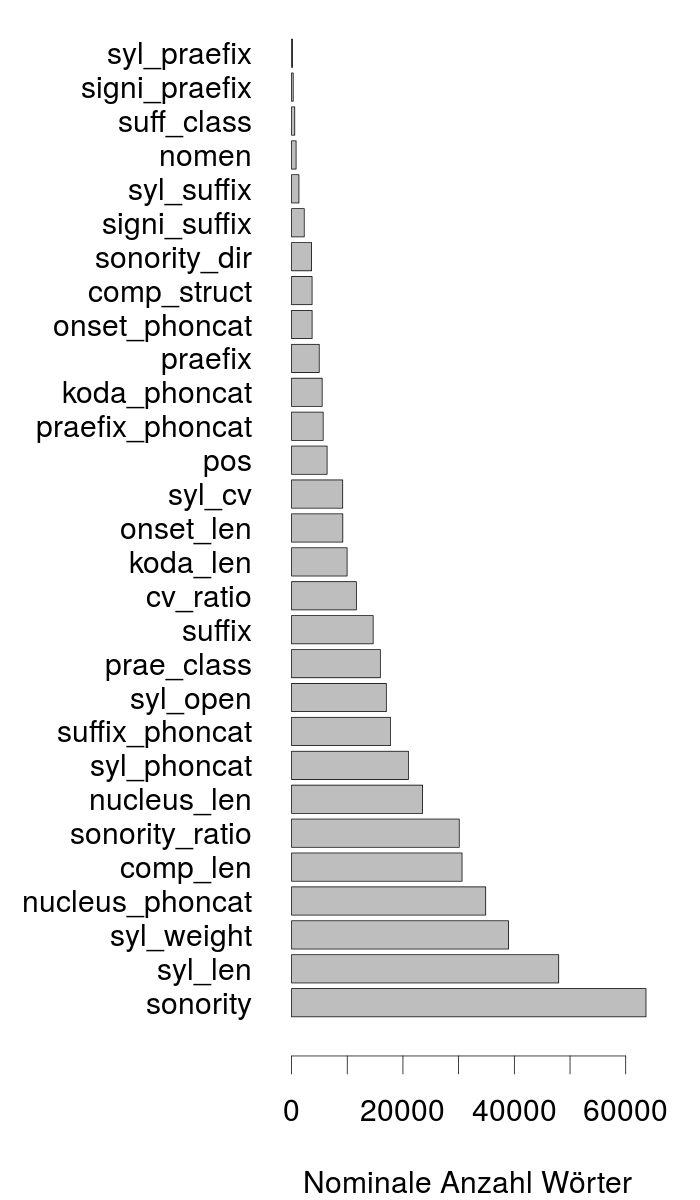
\includegraphics[scale = 0.25]{figures/features/jrip_feature_influence_grouped.png}} {
            \caption{}
            \label{figure:jrip_feature_influence_grouped}
        }
        \ffigbox{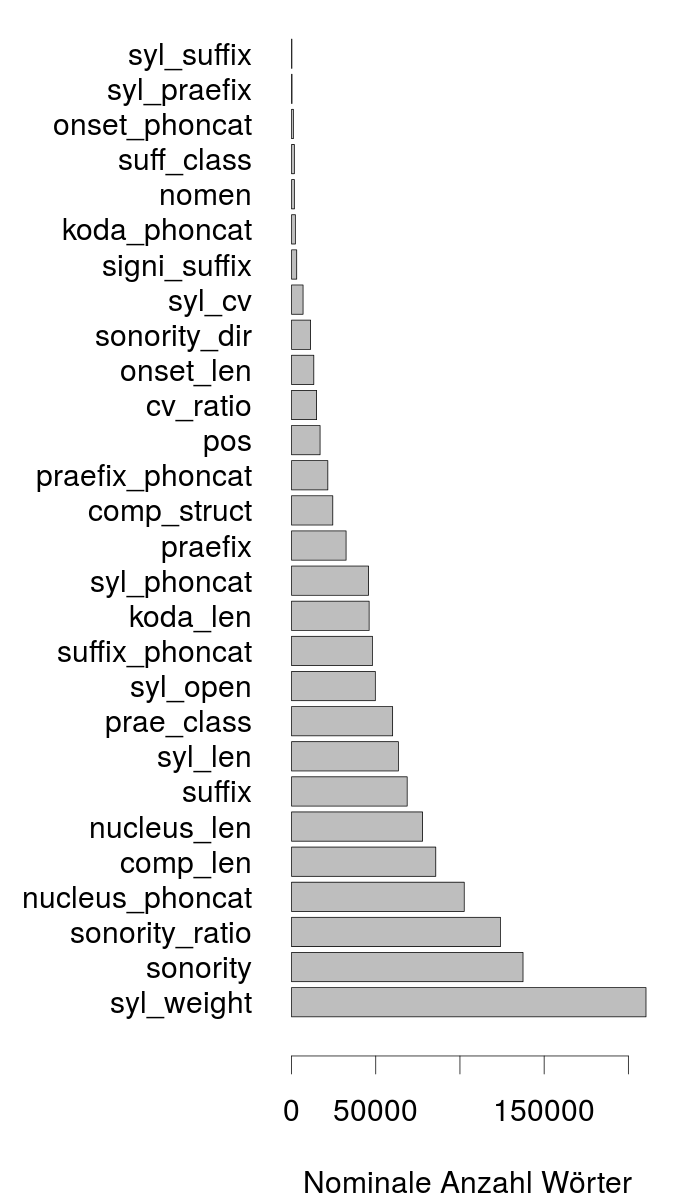
\includegraphics[scale = 0.25]{figures/features/j48_feature_influence_grouped.png}} {
            \caption{}
            \label{figure:j48_feature_influence_grouped}
        }
    \end{floatrow}
\end{figure}

Um den Einfluss der einzelnen Features darstellen zu können, habe ich die Summe der Wörter, 
Die Bedeutung der einzelnen Features für das Gesamtergebnis ist schwierig zu messen. Um dennoch zumindest ein grobes Maß zu erhalten habe ich eine Statistik erstellt, wie viele Wörter von den Regeln erfasst werden, die ein bestimmtes Feature enthalten. Wie bereits erwähnt gibt es bei den Regeln oft ähnliche Varianten, die auf eine große Schnittmenge an selben Wörtern zutreffen. Die Zahlen in Abbildung \label{figure:jrip_feature_influence_grouped} und \label{figure:j48_feature_influence_grouped} sind daher lediglich relativ zueinander zu sehen, die absoluten Zahlen sagen wenig aus. Aus meinen Entscheidungsbäumen habe ich mittels eines kleines R-Skripts Regelsets generiert.

Interessant im Licht der bisherigen Analyse ist, dass die Sonorität und das Silbengewicht die Statistik der JRip-Regeln und Entscheidungsbaum-Regeln anführen. Beim Featureset \texttt{weight} bin ich in Abschnitt \ref{generelles} zu dem Schluss gekommen, das es aufgrund seiner großen Invarianz der Silbenanzahl gegenüber ein recht gut verallgemeinerbares linguistisches Konzept ist. Dies siehe ich durch die häufige Verwendung in einflussreichen Regeln bestätigt. Ähnliches gilt für das grundlegenden Featuresets \texttt{sonority}, das unter Ausschluss anderer Features wenig brauchbar ist, in Kombination aber offensichtlich ein sehr wichtiges Feature darstellt. Die große Bedeutung der Sonorität könnte sich stückweit durch seinen hohen Abstraktionsgrad bei Einbeziehung vieler phonetischer und phonologischer Aspekte sein. Die Sonorität eines Phonems ist eng gekoppelt an seine Phonemklasse und geht dabei weit über die Unterscheidung zwischen Konsonant und Vokal hinaus. Dadurch, dass die Sonorität der Silbe die Summe der Sonorität ihrer Buchstaben ist, sagt die Silbensonorität dabei gleichzeitig auch einiges über die Beschaffenheit der Silbe aus. Zudem ist die Sonorität auch stark mit der Silbenlänge korreliert, die selbst großen Einfluss hat. Je mehr Phoneme die Silbe hat, desto sonoranter kann die Silbe werden. Insgesamt ist die Sonorität ein hervorragendes mittel, viele verschiedene Aspekte einer Silbe numerisch zu repräsentieren.

Mein Feature sonority\_dir, das den Silbensonoritätverlauf über das Wort hinweg repräsentiert scheint hingegen unwichtig zu sein.
Features, die die Suffixe betreffen scheinen wichtiger zu sein als die Präfixe.
Bezüglich der Silbenstruktur ist der Nucleus am wichtigsten, Onset und Koda sind beide recht unwichtig, den Onset jedoch komplett zu ignorieren, wie in der Literatur oft geschieht, sehe ich anhand meiner Daten jedoch nicht gerechtfertigt.



%%%%%%%%%%%%%%%%%
%Welche Features scheinen wichtiger zu sein, welche unwichtiger? Gibt es Features, die immer in Kombination auftreten?
%\subsubsection{Einflussreichste Features}
%\begin{wraptable}{r}{6.5cm}
\tiny
\centering
    \begin{tabular}{|rrr|l|}
    \hline
     $\hat{n}$ & $n$ & $k$ & Feature             \\ \hline
    94                     & 188                & 2                & sonority0        \\
    79,5                   & 159                & 2                & comp\_len        \\
    73                     & 146                & 2                & sonority\_dir    \\
    70                     & 140                & 2                & syl\_len0        \\
    53                     & 106                & 2                & syl\_len1        \\
    49                     & 98                 & 2                & sonority\_ratio0 \\
    46                     & 92                 & 2                & sonority1        \\
    46                     & 92                 & 2                & sonority2        \\
    43                     & 86                 & 2                & sonority3        \\
    41                     & 82                 & 2                & syl\_len2        \\
    36                     & 72                 & 2                & sonority\_ratio1 \\
    34,33                  & 103                & 3                & prae\_class      \\
    33                     & 66                 & 2                & nomen            \\
    32,4                   & 162                & 5                & pos              \\
    32                     & 64                 & 2                & sonority\_ratio2 \\
    30,3                   & 100                & 3,3              & syl\_weight1     \\
    29                     & 58                 & 2                & onset\_len0      \\
    24                     & 48                 & 2                & nucleus\_len1    \\
    23,21                  & 708                & 30,5             & syl\_phoncat1    \\
    23                     & 46                 & 2                & sonority\_ratio3 \\
    23                     & 69                 & 3                & syl\_weight2     \\
    21,03                  & 1912               & 90,9             & suffix3          \\
    20                     & 40                 & 2                & syl\_open2       \\
    20                     & 40                 & 2                & koda\_len1       \\ \hline
    \end{tabular}
    \caption{Normalisierte Häufigkeit der Features in J48-Modellen. Nominalen Häufigkeiten $n$ werden durch den branching factor $k$ zu $\hat{n}=\frac{n}{k}$ normalisiert.}
    \label{table:j48_feature_occurences}
\end{wraptable}
%\begin{table}
    \centering
    \tiny
    \caption{Verwendungshäufigkeit der Features bei allen JRip-Modellen}
    \label{table:jrip_feature_occurences}
    \begin{tabular}{|l|l|} \hline
    Anzahl & Feature \\\hline
     182 & comp\_len         \\
    146  & syl\_weight1      \\
    136  & syl\_len0         \\
    134  & sonority0         \\
    87   & syl\_len1         \\
    81   & prae\_class       \\
    64   & sonority1         \\
    62   & nucleus\_phoncat2 \\
    60   & sonority\_ratio0  \\
    60   & sonority2         \\
    57   & pos               \\
    52   & syl\_weight2      \\
    52   & suff\_class       \\
    48   & syl\_len2         \\
    47   & syl\_phoncat0     \\
    46   & nucleus\_len2     \\
    46   & nucleus\_len1     \\
    45   & onset\_len0       \\
    44   & suffix\_phoncat4  \\
    44   & nucleus\_phoncat1 \\
    43   & sonority3         \\
    35   & syl\_len3         \\
    34   & suffix\_phoncat2  \\
    34   & sonority\_ratio2  \\
    30   & nucleus\_phoncat0 \\
    29   & suffix3           \\
    28   & suffix2           \\
    28   & sonority\_ratio3  \\
    28   & nucleus\_phoncat3 \\
    27   & syl\_open2        \\
    27   & suffix1           \\
    27   & koda\_len2        \\
    27   & cv\_ratio2        \\
    26   & suffix4           \\
    26   & sonority\_ratio1  \\
    26   & nucleus\_len0     \\
    25   & syl\_weight3      \\
    25   & sonority\_dir     \\
    24   & syl\_phoncat3     \\
    23   & syl\_weight0      \\
    23   & syl\_open1        \\
    22   & koda\_len1        \\
    21   & cv\_ratio0        \\
    20   & praefix\_phoncat2 \\
    20   & comp\_struct      \\\hline
    \end{tabular}
\end{table}
%\begin{table}
    \centering
    \small
    \caption{Verwendungshäufigkeit der Features bei allen JRip-Modellen}
    \label{table:jrip_occurences}
    \begin{tabular}{|l|l|}
    \hline
    Jeweils $<$ 10x verwendet	& Jeweils $>$ 25x verwendet \\ \hline
    cv\_ratio4-6	& cv\_ratio2 \\
    syl\_cv4-6	& \\ \hline
    onset\_len1-6	& onset\_len0 \\
    nucleus\_len4-6	& nucleus\_len0-2 \\
    koda\_len3-6	& koda\_len2 \\
    syl\_len5,6 	& syl\_len0-3\\ \hline
    onset\_phoncat0-6 	&  \\
    nucleus\_phoncat4-6 	& nucleus\_phoncat0-3 \\
    koda\_phoncat0,3-6 	&  \\
    syl\_phoncat4-6 	& syl\_phoncat0\\ \hline
    praefix3-5 	& prae\_class \\
    praefix\_phoncat1,3,4,5 	& \\ \hline
    signi\_praefix 	&  \\
    signi\_suffix 	&  \\
    	& suff\_class \\
    	& suffix1-4 \\
    	& suffix\_phoncat2,4\\ \hline
    sonority5,6 	& sonority0-3 \\
    sonority\_ratio4-6 	& sonority\_dir \\
    	& sonority\_ratio0-3\\ \hline
    syl\_open4-6 	& syl\_open2 \\
    syl\_weight5,6 	& syl\_weight1-3\\ \hline
    nomen 	&  \\
    	& comp\_len \\
    	& pos \\ \hline
    \end{tabular}
\end{table}

%\subsubsection{Wenig einflussreiche  Features}
%\begin{wraptable}{r}{5cm}
    \centering
    \tiny
    \caption{Von JRip/J48 auf keinem Trainingsset benutze Features}
    \label{table:unused_features}
    \begin{tabular}{|l|l|}
    \hline
    {\bf J48}	 & {\bf JRip} \\\hline
    cv\_ratio4	&  \\
    cv\_ratio5	&  \\
    cv\_ratio6	 & cv\_ratio6\\\hline
    koda\_len5	 & koda\_len5 \\
    koda\_len6	 & koda\_len6\\\hline
    koda\_phoncat0	&  \\
    koda\_phoncat3	&  \\
    koda\_phoncat4	&  \\
    koda\_phoncat5	 & koda\_phoncat5 \\
    koda\_phoncat6	 & koda\_phoncat6\\\hline
    nucleus\_phoncat5	 & \\\hline
                    	 & nucleus\_phoncat6\\\hline
    onset\_len5	 & onset\_len5 \\
    onset\_len6	 & onset\_len6\\\hline
    onset\_phoncat2	&  \\
    onset\_phoncat3	&  \\
    onset\_phoncat4	&  \\
    onset\_phoncat5	 & onset\_phoncat5 \\
    onset\_phoncat6	 & onset\_phoncat6\\\hline
    sonority6	 & sonority6\\\hline
    sonority\_ratio6	 & sonority\_ratio6\\\hline
    syl\_cv4	&  \\
    syl\_cv6	 & syl\_cv6\\\hline
    	 & syl\_len5 \\
    syl\_len6	 & syl\_len6\\\hline
    syl\_open5	&  \\
    syl\_open6	 & syl\_open6\\\hline
    syl\_phoncat5	 & syl\_phoncat6 \\
    	 & syl\_weight6 \\
    	 & nucleus\_len6 \\\hline
    \end{tabular}
\end{wraptable}
%26 Features wurden über alle 6 Trainingssets hinweg, egal auf welchem Featureset, von keinem einzigen J48 berücksichtigt (Tabelle \ref{table:unused_features}). JRip hat erstaunlicherweise lediglich 19 Features nie berücksichtigt. Bis auf zwei Features, die JRip alleinig nie beachtet hat, decken sich jedoch die Features. Generell sind das Features, die sich auf die hinteren Silben beziehen, die 5, 6, 7. Das ist nicht verwunderlich, da diese Attribute zu kleineren Trainingssets gehören, so dass es schwieriger ist dort Gesetzmä0igkeiten zu erkennen. Ausnahmen hiervon sind koda\_phoncat0 und koda\_phoncat3 und onset\_phoncat2

%\subsubsection{Einflussreichste JRip-Regeln}
%Sämtliche von JRip erzeugte Regeln habe ich mittels eines Shell-Skriptes nach Anzahl der Samples sortiert, auf die diese Regel zutrifft. Die Liste wird von folgender Regel für Dreisilber auf dem \texttt{numeric}-Featureset angeführt:
%\begin{align*}
%\texttt{(comp\_len <= 1) and (sonority\_ratio0 <= 3) and (syl\_len0 <= 3) and}\\
%\texttt{(onset\_len0 >= 1) and (nucleus\_len0 <= 1) and (koda\_len0 <= 0)}\\
%\texttt{=> stress\_class=paenultima}
%\end{align*}
%Dies Regel trifft auf alle 634 Wörter aus dem Testset zu, ohne eine Ausnahme. Das sind immerhin fast 37\% aller Wörter des Testsets mit Paenultima-Betonung. Mit sechs Bedingungen erscheint sie nur mäßig Ausdrucksstark, doch lassen sich aus ihr einige interessante Dinge ableiten. Diese Regel gilt für Nonkomposita (comp\_len <= 1) und betrifft ausschließlich Eigenschaften der ersten Silbe (index 0). Die erste Silbe darf keine Koda haben (koda\_len0 <= 0), muss also offen sein, und der Onset darf nicht leer sein (onset\_len0 >= 1). Der Nucleus des Präfix darf nur aus genau einem Sonoranten bestehen (nucleus <= 1), da jede Silbe einen Nucleus haben muss. Die Silbe darf maximal drei Phoneme enthalten (syl\_len0 <= 3), was bei genau einem Nucleus und ohne Koda eine Onsetlänge von 1 oder 2 ergibt. Die durchschnittliche Sonorität pro Phonem der Silbe muss dabei $\leq3$ sein. Ein Blick in Tabelle \ref{table:sonority} der Sonoritätsklassen zeigt, dass Offene Vokale und Diphtonge mit einer Sonorität von je 10 damit nicht in Wörtern dieser Regel zu finden sein können. 

%(comp_len <= 1) and (cv_ratio0 >= 2) and (sonority0 <= 11) and (syl_len0 <= 3) and (nucleus_len1 >= 2) => stress_class=paenultima (596.0/54.0)

%(comp_len <= 1) and (cv_ratio0 >= 2) and (syl_len0 <= 3) and (sonority_ratio0 <= 3) and (sonority0 >= 11) and (sonority1 >= 12) => stress_class=paenultima (304.0/3.0)


%78\% der Ultimabetonungen bei Dreisilbern werden hiermit erklärt (+6.7\% FP). Der Nucleus der letzten Silbe muss wieder ein Langvokal oder Diphtong sein und mindestens einen Konsonanten enthalten. Hinzu kommt noch, dass die zweite Silbe nur ein oder zwei Phoneme haben darf und die erste Silbe einen Onset haben muss. Diesen beiden sehr guten Regeln gemein ist jedoch die Forderung nach einem Langvokal oder Diphtong in der Ultima. Zwei ähnliche Regeln finden sich auch für Viersilber: Longvokal/Diphtong in der ultima, die Silbe davor maximal zwei Phoneme lang. Die eine Regel fordert dann eine geschlossene 2. Silbe, die andere eine geschlossene letzte Silbe, wobei der Unterschied im Ergebnis minimal ist, also es sich wahrscheinlich lediglich um Koinzidenzien handelt. Festzuhalten ist unzweifelhaft, dass ein Langvokal/Diphtong im Suffix den Akzent anzieht, sofern die Silbe davor recht kurz ist.

%\subsection{Evaluation der Featuresets}

%\begin{center}{
%    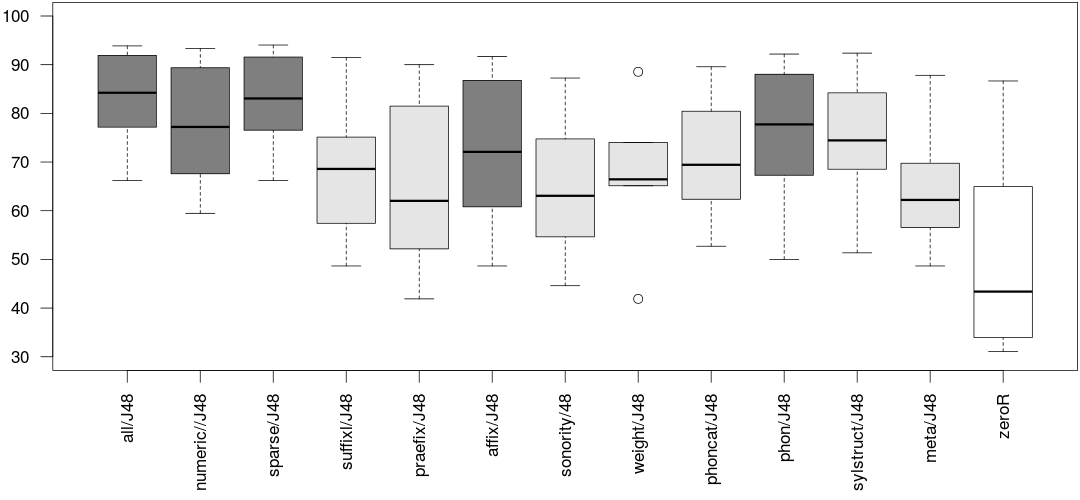
\includegraphics[width=.75\columnwidth]{figures/featuresets/J48.png}
%    \label{figure:featuresets_J48}
%}\end{center}




%\begin{center}{
%    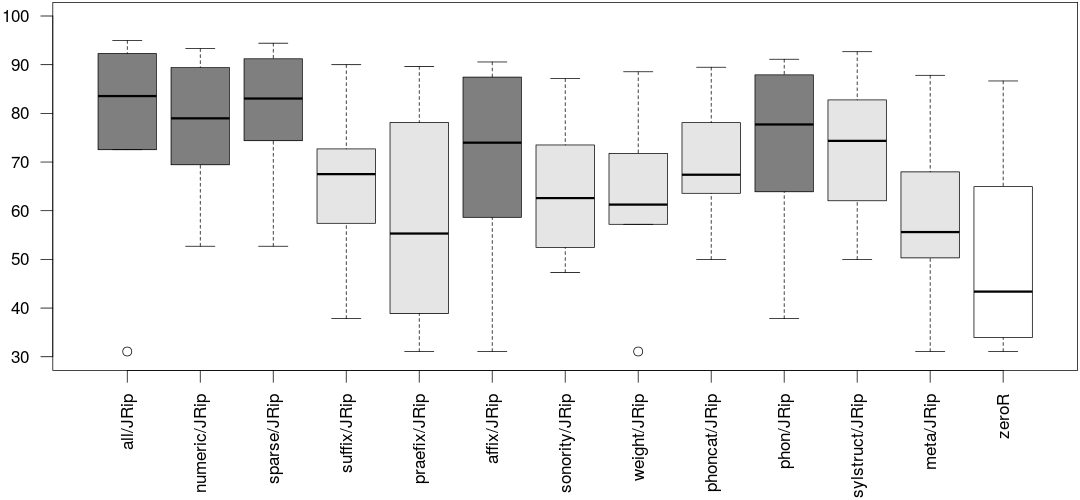
\includegraphics[width=.75\columnwidth]{figures/featuresets/JRip.png}
%    \label{figure:featuresets_JRip}
%}\end{center}

%\begin{center}{
%    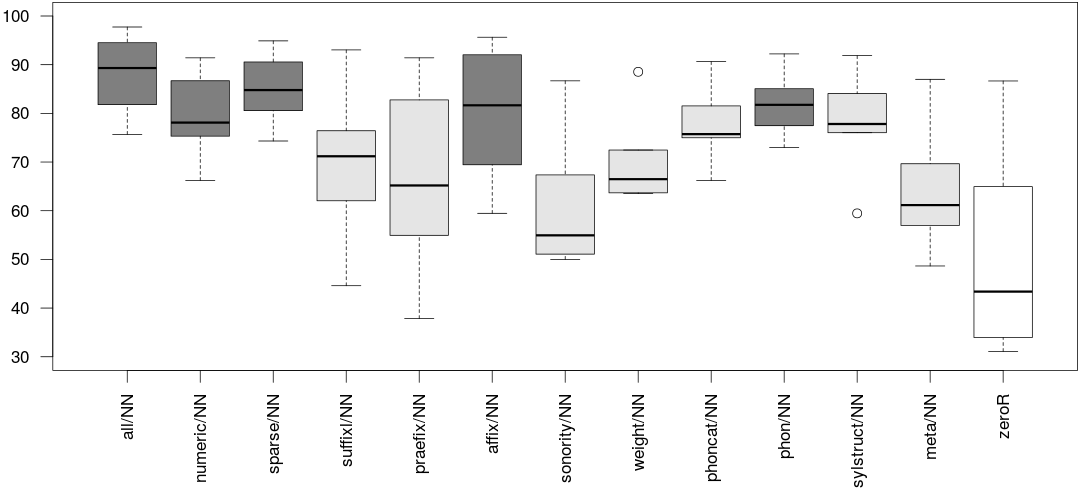
\includegraphics[width=.75\columnwidth]{figures/featuresets/NN.png}
%    \label{figure:featuresets_NN}
%}\end{center}





\subsection{Vergleich zu bisherigen Arbeiten}
%Wie fügt sich meine Arbeit in die Wissenslandschaft ein?

Anzahl Regeln \cite{Rapp1995}

Ergebnisse rein nominal hinter \cite{Hain2004} mit 97.4\%, jedoch hatte er viele Flektionsformen und mehr Daten. Außerdem bei einer 1-to-n Kodierung der Phoneme rund über 400 Inputs (über 40 Phoneme, erste 9 Phoneme).

Daten nicht unbedingt repräsentativ für echten Text, da alle CELEX-Wörter gleichgewichtet. In Realität komische Wörter seltener, daher vmtl besser. Probleme vmtl bei Namen, Fremdwörter sind schwieriger und Komposita.

Nur für Deutsch, Methode lässt sich adaptieren, Ergebnisse nicht. Vielversprehcend jedoch.

Phonemische/Lexikalische Regeln schlecht falls OOV, numerische Werte sehr gut, da immer anwendbar.

Mehr Daten aus wordforms zB wäre sinnvoll, da Erkennungsrate steigt mit Wortanzahl, kein Sättigung \cite[S.~123]{Dou&Bergsma2009}.
Keine linguistischen Regeln, nur statistik, viele Features, mehr Daten. \cite{Dou&Bergsma2009}

%In der Literatur wird häufig Wert darauf gelegt, dass Trainings und Testdaten nicht die gleichen Wortstämme enthalten, damit nicht mit 'sagt' trainiert und mit 'sagen' getestet wird, was möglicherweise die Ergebnisse beeinflussen würde, da die Flektion die betonte Silbe nicht ändert. [ZITAT] Da meine Daten jedoch allesamt Lemmata sind, sind ihre Wortstämme meist verschieden. In meinen Trainings- und Testdaten finden sich insgesamt 2137 Wortstämme, die nicht einzigartig sind, in der Summe sind das 4549 (8,9\%) Wörter.

%%%%%%%%%%%%%%%%%%%%%%%%%%%%%%%%%%%%%%
%%%%%%%%%%%%%%%%%%%%%%%%%%%%%%%%%%%%%%
%%%%%%%%%%%%%%%%%%%%%%%%%%%%%%%%%%%%%%

%In mehr als der Hälfte der Fälle liefern die Neuronalen Netze die besten Ergebnisse, insbesondere auf Featuresets mit vielen verschiednen Werten. J48 ist in den meisten Fällen etwas besser als JRip, große Unterschiede sind recht selten. Die besseren Ergebnisse der NN im Vergleich zu J48, das wiederum leicht besser ist als JRip, lassen sich wahrscheinlich durch die Fähigkeit der Lernalgorithmen erklären, Details zu lernen.


%Paarweise disjunkte Featuresets entsprechend der Betrachutngsebenen         affix   phon    sylstruct   meta            
%(Variante zur differenzierung zwischen Prä und Suffix)                      praefix suffix  phon        sylstruct   meta
%Erweiterung einer sparsamen Grundmenge um hochdimensionale Attribute        all     sparse  numeric             
%Vergleich größter paarweise disjunkter Featuresets                          numeric affix   phoncat     weight          
%Vergleich phonetischer Attribute                                            phoncat weight  sonority                
%Vergleich kleinster paarweise disjunkter Featuresets                        praefix suffix  phoncat     weight      sonority    sylstruct   meta

\newpage

%%
\chapter{Zusammenfassung und Ausblick}
%%%%%%%%%%%%%%%%%%%%%%%%%
% Was war das Ziel?
% Was habe ich getan?
% Was wurde erreicht?
% Was lernen wir daraus?
% "Woran könnte man weiter forschen?"
%%%%%%%%%%%%%%%%%%%%%%%%%

93.4\% all/NN
zur Analyse sinnvoll auch Modelle mit geringeren Erekkungsraten zu untersuchen, die jedoch 




















Ziel dieser Arbeit war die Vorhersage des lexikalischen Wortakzentes mit linguistischen Features und symbolischen Lernverfahren. Ich habe dazu verschiedene linguistische Konzepte als Features verwendet und diese in verschiedenen Featuresets kombiniert. Auf basis der Lemmata aus dem CELEX habe ich drei verschiedene Lernalgorithmen trainiert: Entscheidungsbäume (C4.5), Inductive Rule Learning (JRip) und Neural Networks. Mit allen drei Algorithmen war ich in der Lage den Betonungsklasse in über 90\% der Fälle richtig zu bestimmen. Mit insgesamt 93.4\% erreichten Neural Networks die beste Ergebnisse auf allen verfügbaren Features.

 





%%%%%%%%%%%%%%%%%%%%%%%%%%%%

\section{Ausblick}
Alternativ zum gewählten Ansatz zur Klassifizierung der Betonungsmuster wäre es auch möglich keine diskreten Klassen, sondern eine reele Zahl $x \in [-1,1]$ zu bestimmen, die die Position der Betonung angibt. Die Silben eines $n$-silbigen Wortes teilen dieses Intervall in $n$ uniforme Teilintervalle $s_i$. Ist $x \in s_i$, so ist die i-te Silbe betont. So wäre es nicht notwendig die Trainingsdaten entsprechend ihrer Silbenzahl aufzuteilen und würde allgemeinere Regeln erhalten.

Wie in Abschnitt \ref{rule_simplify} demonstriert kann man viele Regeln mit etwas Hintergrundwissen deutlich kompakter Schreiben. Mittels logischer Programmiersprachen wie Prolog ist es möglich Algorithmen zu schreiben, die ausgehend von einer gegebenen Wissensbasis neue logische Schlüsse ziehen \cite[S.~706]{RusselNorvig}. Ich halte es für sehr vielversprechend Domänenwissen aus der Linguistik und maschinelles Lernen so noch enger zu verweben.

Weka optimieren um Ergebnisse der Klassifikation besser zu analysieren. Fehlerwörter bei JRip-Regeln etc.
Weka hat sich während meiner Arbeit als ein sehr mächtiges und zum Teil recht störrisches Werkzeug erwiesen. Leider hört Weka dort auf, wo es eigentlich spannend wird: Bei der Interpretation der Ergebnisse. Es wäre höchstpraktisch sich die Wörter anzeigen lassen zu können, die von einer JRip-Regel oder einem Blatt im Entscheidungsbaum erfasst werden. 

% Esemble
\newpage

%%
\renewcommand{\thesection}{\Alph{section}}%
\appendix 
\addcontentsline{toc}{chapter}{Anhang} 

%%%%%%%%%%%%%%%%%%%%%%%%
%%%%%%%%%%%%%%%%%%%%%%%%
%%%%%%%%%%%%%%%%%%%%%%%%

\section{Studie zu Affixen}
\label{affix_studie}
Zur Identifizierung möglichst vieler relevanter Prä- und Suffixe habe ich eine kleine Studie zu betonten/unbetonten Affixen durchgeführt. Hierfür habe ich einen Entscheidungsbaum mittels REPTree aus WEKA auf dem kompletten Datensatz (ohne Komposita) je Silbe trainiert. Als Features dienten mir lediglich die Suffixe bzw. Präfixe.  
Ich habe deutlich mehr Suffixe als Präfixe gefunden, die eine eindeutige Betonungsklasse identifizieren. Aus allen Affixen habe ich die mit weniger als 10\% Ausnahmen identifiziert.
Datensätze mit wenigen Silben haben mehr eindeutig betonte oder unbetonte Affixe. Bemerkenswert ist, dass es bei den Wörtern mit mehr als 3 Silben kein signifikantes Affix gibt, dass sich nicht schon bei den Zwei- und Dreisilbern als wichtig herausgestellt hat. Man kann jedoch bei einigen Affixen feststellen, dass sie häufiger eindeutig betont/unbetont sind als andere, beispielsweise -ik und -ismus. Ich vermute dass bei kurzen Wörtern es weniger andere Phänomene auftreten können, als bei langen Wörtern. Dies wäre ein Indiz für die sogenannte XYZ Hypothese, wie sie unter anderem in [CITE] formuliert wurde. Darüber hinausgehend formuliere ich die Hypothese, dass es nicht nur betonte und unbetonte Affixe gibt wie in [CITE] angegeben, sondern verschiedene Grade an Anzieungskraft der Betonung gibt. Ausgehend von der Hypothese, dass mehrere Betonungsregeln in wechselseitiger Beziehung zu einer stehen erscheint es um so sinnvoller neben Entscheidungsbäumen und Propositional Rule Learnern auch nichtlineare Neuronale Netze in die Untersuchung mit einzubeziehn, die im gegensatz zu den beiden erstgenannten Verfahren diese interdependeznen abbilden können.
\begin{table}[h]
\centering
\caption{Betonte Präfixe in Nonkomposita}
\resizebox{\columnwidth}{!}{%
\begin{tabular}{|l|lllllllllllllllllllllll|}
\hline
{\bf Silben} & \multicolumn{23}{c|}{{\bf Betontes Präfixe}} \\ \hline
2	& ab	& ~	& auf	& aus	& bei	& durch	& ein	& fern	& fort	& gegen	& hinter	& hin	& hoch	& mit	& nach	& ueber	& um	& unter	& ur	& vor	& weg	& ~	& \\ 
3	& ab	& an	& auf	& aus	& ~	& ~	& ein	& fern	& fort	& gegen	& hinter	& hin	& hoch	& mit	& nach	& ueber	& ~	& unter	& ur	& vor	& weg	& zu\\ 
4	& ab	& an	& auf	& aus	& ~	& durch	& ein	& fern	& fort	& ~	& ~	& ~	& ~	& mit	& nach	& ~	& ~	& ~	& ur	& ~	& 	& ~	& \\ 
5	& ~	& an	& auf	& aus	& ~	& ~	& ein	& ~	& ~	& gegen	& hinter	& ~	& hoch	& mit	& ~	& ~	& um	& ~	& ur	& ~	& 	& ~	& \\ 
6	& ab	& ~	& auf	& aus	& ~	& ~	& ~	& ~	& ~	& ~	& ~	& ~	& ~	& ~	& ~	& ueber	& um	& unter	& ~	& 	& ~	& \\  \hline
$\Rightarrow$	& ab	& an	& auf	& aus	& bei	& durch	& ein	& fern	& fort	& gegen	& hinter	& hin	& hoch	& mit	& nach	& ueber	& um	& unter	& ur	& vor	& weg	& zu \\ \hline
\end{tabular}%
}
\end{table}
\begin{table}[h]
\centering
\small
\caption{Unbetonte Suffixe in Nonkomposita}
\resizebox{\columnwidth}{!}{%
\begin{tabular}{|l|llllllllllllllll|}
\hline
{\bf Silben}     & \multicolumn{16}{c|}{{\bf Betontes Suffixe}} \\ \hline
2                & ig &  ik  &         &  bar    & er   & sam & ung & isch & lich & heit & ler   & ling & schaft & nis    & tum  & ~     \\
3                & ig &  ik  &   ismus &  ~      & ~    &    ~&  ~   &   ~ &     ~ &  ~   &    ~ & ling & ~      &  nis   & tum  & keit  \\
4                & ~  &  ik  &   ismus &  ~      & ~    &    ~&  ~   &   ~ &     ~ &  ~   &  ~   &  ~   & ~      &    ~   & ~    & ~     \\
5                &    &  ik  &   ismus &  ~      & ~    &    ~&   ~  &   ~ &  ~    & ~    &  ~   & ~    &    ~   &  ~     & tum  & ~     \\
6                & ig &  ik  &   ismus &  ~      & ~    &    ~&   ~  &   ~ & lich  & ~    &  ler & ~    &  ~     & ~      & tum  & ~     \\ \hline
$\Rightarrow$    & ig &  ik  &   ismus &  ~	     & ~	&    ~&   ~  &   ~ & lich  & ~    & ler  & ling & ~      &  nis   & tum  & keit  \\ \hline
\end{tabular}%
}
\end{table}
\begin{table}[h]
\centering
\caption{Unbetonte Präfixe in Nonkomposita}
\begin{tabular}{|l|lllll|}
\hline
{\bf Silben}       & \multicolumn{5}{c|}{{\bf Unbetontes Suffixe}} \\ \hline
2                  & be-     & ent-   & er-   & ver-   & zer-   \\
3                  & be-     & ent-   & er-   & ver-   & zer-   \\
4                  & be-     & ent-   & er-   & ver-   & zer-   \\
5                  & be-     &        & er-   & ver-   &        \\
6                  & be-     &        & er-   &        &        \\ \hline
{\bf Als Feature:} & be-     & ent-   & er-   & ver-   & zer-  \\ \hline
\end{tabular}
\end{table}
\begin{table}[h]
\centering
\caption{Betonte Suffixe bei Nonkomposita}
\begin{tabular}{|l|cc|}
\hline
{\bf Silben}       & \multicolumn{2}{c|}{{\bf Betontes Suffixe}} \\ \hline
2                  &                      &                     \\
3                  & -ist                 & -ei                 \\
4                  & -ist                 & -ei                 \\
5                  & -ist                 & -ei                 \\
6                  & -ist                 &                     \\ \hline
{\bf Als Feature:} & -ist                 & -ei                 \\ \hline
\end{tabular}
\end{table}


%%%%%%%%%%%%%%%%%%%%%%%%

\section{Features und Featuresets}
\label{detail_performance}
Die Summen am Ende der Tabelle beziehen sich auf die Anzahl der Werte aller Features eines Featuresets. Numerische Attribute Zählen als $1$. So gesehen ist die entsprechende Summe gleich der Anzahl an Neuronen im Input-Layer des Neuronalen Netzes.
\footnotesize
\begin{longtable}{|r|llllll|c|}

    \caption{Anzahl Werte je Attribut}
    \label{table:feature_dimensions}\\
    
    \hline
    \diagbox{{\bf Attribut}}{{\bf Silben}} & 2 & 3 & 4 & 5 & 6 & 7 & Erwartungswert \\ \hline
    syl\_suffix       & 54   & 94   & 65   & 22   & 5    & 2    & 68,4     \\
    signi\_suffix     & 23   & 37   & 29   & 20   & 13   & 9    & 29,4     \\
    suffix1           & 23   & 22   & 21   & 21   & 18   & 12   & 21,8     \\
    suffix2           & 71   & 71   & 47   & 22   & 9    & 2    & 59,5     \\
    suffix3           & 94   & 116  & 80   & 21   & 8    & 2    & 90,9     \\
    suffix4           & 42   & 115  & 60   & 17   & 8    & 2    & 72,1     \\
    suffix5           & 28   & 144  & 71   & 23   & 8    & 3    & 83,1     \\
    suffix\_phoncat1  & 6    & 6    & 6    & 6    & 5    & 5    & 6        \\
    suffix\_phoncat2  & 11   & 11   & 9    & 7    & 6    & 3    & 10       \\
    suffix\_phoncat3  & 21   & 25   & 19   & 12   & 7    & 2    & 20,9     \\
    suffix\_phoncat4  & 30   & 32   & 24   & 17   & 9    & 2    & 27,7     \\
    suffix\_phoncat5  & 31   & 45   & 36   & 22   & 6    & 2    & 36,3     \\
    suff\_class       & 3    & 3    & 3    & 3    & 3    & 3    & 3        \\
    syl\_praefix      & 45   & 102  & 94   & 37   & 4    & 1    & 77,3     \\
    signi\_praefix    & 23   & 24   & 22   & 20   & 14   & 5    & 22,6     \\
    praefix1          & 50   & 50   & 50   & 49   & 45   & 36   & 49,7     \\
    praefix2          & 107  & 130  & 86   & 25   & 2    & 1    & 101,4    \\
    praefix3          & 30   & 86   & 42   & 11   & 1    & 1    & 52,6     \\
    praefix4          & 26   & 106  & 37   & 7    & 1    & 1    & 58,1     \\
    praefix5          & 10   & 35   & 18   & 6    & 1    & 1    & 21,2     \\
    praefix\_phoncat1 & 6    & 6    & 6    & 5    & 5    & 5    & 5,9      \\
    praefix\_phoncat2 & 12   & 12   & 12   & 9    & 7    & 4    & 11,6     \\
    praefix\_phoncat3 & 24   & 29   & 28   & 17   & 8    & 4    & 25,9     \\
    praefix\_phoncat4 & 42   & 52   & 40   & 21   & 13   & 2    & 42,9     \\
    praefix\_phoncat5 & 52   & 76   & 52   & 27   & 11   & 1    & 58,2     \\
    prae\_class       & 3    & 3    & 3    & 3    & 3    & 3    & 3        \\
    sonority0         & 1    & 1    & 1    & 1    & 1    & 1    & 1        \\
    sonority1         & 1    & 1    & 1    & 1    & 1    & 1    & 1        \\
    sonority2         & ~    & 1    & 1    & 1    & 1    & 1    & 1        \\
    sonority3         & ~    & ~    & 1    & 1    & 1    & 1    & 1        \\
    sonority4         & ~    & ~    & ~    & 1    & 1    & 1    & 1        \\
    sonority5         & ~    & ~    & ~    & ~    & 1    & 1    & 1        \\
    sonority6         & ~    & ~    & ~    & ~    & ~    & 1    & 1        \\
    sonority\_ratio0  & 1    & 1    & 1    & 1    & 1    & 1    & 1        \\
    sonority\_ratio1  & 1    & 1    & 1    & 1    & 1    & 1    & 1        \\
    sonority\_ratio2  & ~    & 1    & 1    & 1    & 1    & 1    & 1        \\
    sonority\_ratio3  & ~    & ~    & 1    & 1    & 1    & 1    & 1        \\
    sonority\_ratio4  & ~    & ~    & ~    & 1    & 1    & 1    & 1        \\
    sonority\_ratio5  & ~    & ~    & ~    & ~    & 1    & 1    & 1        \\
    sonority\_ratio6  & ~    & ~    & ~    & ~    & ~    & 1    & 1        \\
    sonority\_dir     & 1    & 1    & 1    & 1    & 1    & 1    & 1        \\
    syl\_weight0      & 3    & 3    & 3    & 3    & 3    & 3    & 3        \\
    syl\_weight1      & 4    & 3    & 3    & 3    & 3    & 3    & 3,3      \\
    syl\_weight2      & ~    & 3    & 3    & 3    & 3    & 3    & 3        \\
    syl\_weight3      & ~    & ~    & 4    & 3    & 3    & 3    & 3,7      \\
    syl\_weight4      & ~    & ~    & ~    & 4    & 3    & 3    & 3,8      \\
    syl\_weight5      & ~    & ~    & ~    & ~    & 3    & 3    & 3        \\
    syl\_weight6      & ~    & ~    & ~    & ~    & ~    & 3    & 3        \\
    syl\_open0        & 2    & 2    & 2    & 2    & 2    & 2    & 2        \\
    syl\_open1        & 3    & 2    & 2    & 2    & 2    & 2    & 2,3      \\
    syl\_open2        & ~    & 2    & 2    & 2    & 2    & 2    & 2        \\
    syl\_open3        & ~    & ~    & 3    & 2    & 2    & 2    & 2,7      \\
    syl\_open4        & ~    & ~    & ~    & 3    & 2    & 2    & 2,8      \\
    syl\_open5        & ~    & ~    & ~    & ~    & 2    & 2    & 2        \\
    syl\_open6        & ~    & ~    & ~    & ~    & ~    & 2    & 2        \\
    syl\_phoncat0     & 37   & 40   & 30   & 18   & 8    & 5    & 34,1     \\
    syl\_phoncat1     & 33   & 36   & 26   & 17   & 9    & 4    & 30,5     \\
    syl\_phoncat2     & ~    & 32   & 30   & 18   & 10   & 4    & 28,9     \\
    syl\_phoncat3     & ~    & ~    & 22   & 16   & 11   & 5    & 19,6     \\
    syl\_phoncat4     & ~    & ~    & ~    & 14   & 7    & 3    & 12,1     \\
    syl\_phoncat5     & ~    & ~    & ~    & ~    & 8    & 5    & 7,4      \\
    syl\_phoncat6     & ~    & ~    & ~    & ~    & ~    & 5    & 5        \\
    onset\_phoncat0   & 6    & 5    & 6    & 5    & 4    & 4    & 5,5      \\
    onset\_phoncat1   & 7    & 5    & 5    & 5    & 5    & 3    & 5,5      \\
    onset\_phoncat2   & ~    & 5    & 6    & 6    & 4    & 3    & 5,4      \\
    onset\_phoncat3   & ~    & ~    & 6    & 5    & 3    & 3    & 5,5      \\
    onset\_phoncat4   & ~    & ~    & ~    & 6    & 5    & 4    & 5,7      \\
    onset\_phoncat5   & ~    & ~    & ~    & ~    & 3    & 3    & 3        \\
    onset\_phoncat6   & ~    & ~    & ~    & ~    & ~    & 2    & 2        \\
    koda\_phoncat0    & 8    & 8    & 7    & 6    & 6    & 3    & 7,5      \\
    koda\_phoncat1    & 9    & 7    & 6    & 5    & 4    & 3    & 7        \\
    koda\_phoncat2    & ~    & 7    & 7    & 4    & 5    & 3    & 6,6      \\
    koda\_phoncat3    & ~    & ~    & 8    & 4    & 4    & 3    & 6,7      \\
    koda\_phoncat4    & ~    & ~    & ~    & 7    & 3    & 3    & 6        \\
    koda\_phoncat5    & ~    & ~    & ~    & ~    & 5    & 2    & 4,4      \\
    koda\_phoncat6    & ~    & ~    & ~    & ~    & ~    & 3    & 3        \\
    nucleus\_phoncat0 & 4    & 4    & 4    & 4    & 3    & 3    & 4        \\
    nucleus\_phoncat1 & 5    & 4    & 4    & 4    & 4    & 3    & 4,3      \\
    nucleus\_phoncat2 & ~    & 4    & 4    & 4    & 3    & 3    & 4        \\
    nucleus\_phoncat3 & ~    & ~    & 5    & 4    & 4    & 3    & 4,7      \\
    nucleus\_phoncat4 & ~    & ~    & ~    & 5    & 3    & 3    & 4,5      \\
    nucleus\_phoncat5 & ~    & ~    & ~    & ~    & 3    & 3    & 3        \\
    nucleus\_phoncat6 & ~    & ~    & ~    & ~    & ~    & 4    & 4        \\
    syl\_len0         & 1    & 1    & 1    & 1    & 1    & 1    & 1        \\
    syl\_len1         & 1    & 1    & 1    & 1    & 1    & 1    & 1        \\
    syl\_len2         & ~    & 1    & 1    & 1    & 1    & 1    & 1        \\
    syl\_len3         & ~    & ~    & 1    & 1    & 1    & 1    & 1        \\
    syl\_len4         & ~    & ~    & ~    & 1    & 1    & 1    & 1        \\
    syl\_len5         & ~    & ~    & ~    & ~    & 1    & 1    & 1        \\
    syl\_len6         & ~    & ~    & ~    & ~    & ~    & 1    & 1        \\
    koda\_len0        & 1    & 1    & 1    & 1    & 1    & 1    & 1        \\
    koda\_len1        & 1    & 1    & 1    & 1    & 1    & 1    & 1        \\
    koda\_len2        & ~    & 1    & 1    & 1    & 1    & 1    & 1        \\
    koda\_len3        & ~    & ~    & 1    & 1    & 1    & 1    & 1        \\
    koda\_len4        & ~    & ~    & ~    & 1    & 1    & 1    & 1        \\
    koda\_len5        & ~    & ~    & ~    & ~    & 1    & 1    & 1        \\
    koda\_len6        & ~    & ~    & ~    & ~    & ~    & 1    & 1        \\
    onset\_len0       & 1    & 1    & 1    & 1    & 1    & 1    & 1        \\
    onset\_len1       & 1    & 1    & 1    & 1    & 1    & 1    & 1        \\
    onset\_len2       & ~    & 1    & 1    & 1    & 1    & 1    & 1        \\
    onset\_len3       & ~    & ~    & 1    & 1    & 1    & 1    & 1        \\
    onset\_len4       & ~    & ~    & ~    & 1    & 1    & 1    & 1        \\
    onset\_len5       & ~    & ~    & ~    & ~    & 1    & 1    & 1        \\
    onset\_len6       & ~    & ~    & ~    & ~    & ~    & 1    & 1        \\
    nucleus\_len0     & 1    & 1    & 1    & 1    & 1    & 1    & 1        \\
    nucleus\_len1     & 1    & 1    & 1    & 1    & 1    & 1    & 1        \\
    nucleus\_len2     & ~    & 1    & 1    & 1    & 1    & 1    & 1        \\
    nucleus\_len3     & ~    & ~    & 1    & 1    & 1    & 1    & 1        \\
    nucleus\_len4     & ~    & ~    & ~    & 1    & 1    & 1    & 1        \\
    nucleus\_len5     & ~    & ~    & ~    & ~    & 1    & 1    & 1        \\
    nucleus\_len6     & ~    & ~    & ~    & ~    & ~    & 1    & 1        \\
    syl\_cv0          & 19   & 19   & 17   & 13   & 8    & 4    & 17,7     \\
    syl\_cv1          & 17   & 19   & 15   & 11   & 9    & 3    & 16,6     \\
    syl\_cv2          & ~    & 18   & 17   & 12   & 8    & 3    & 16,6     \\
    syl\_cv3          & ~    & ~    & 15   & 10   & 8    & 3    & 13,1     \\
    syl\_cv4          & ~    & ~    & ~    & 10   & 6    & 3    & 8,9      \\
    syl\_cv5          & ~    & ~    & ~    & ~    & 8    & 3    & 7,1      \\
    syl\_cv6          & ~    & ~    & ~    & ~    & ~    & 7    & 7        \\
    cv\_ratio0        & 1    & 1    & 1    & 1    & 1    & 1    & 1        \\
    cv\_ratio1        & 1    & 1    & 1    & 1    & 1    & 1    & 1        \\
    cv\_ratio2        & ~    & 1    & 1    & 1    & 1    & 1    & 1        \\
    cv\_ratio3        & ~    & ~    & 1    & 1    & 1    & 1    & 1        \\
    cv\_ratio4        & ~    & ~    & ~    & 1    & 1    & 1    & 1        \\
    cv\_ratio5        & ~    & ~    & ~    & ~    & 1    & 1    & 1        \\
    cv\_ratio6        & ~    & ~    & ~    & ~    & ~    & 1    & 1        \\
    pos               & 5    & 5    & 5    & 5    & 4    & 4    & 5        \\
    comp\_struct      & 13   & 18   & 17   & 14   & 8    & 2    & 15,8     \\
    nomen             & 2    & 2    & 2    & 2    & 2    & 2    & 2        \\
    comp\_len         & 1    & 1    & 1    & 1    & 1    & 1    & 1        \\
    stress\_class     & 2    & 3    & 4    & 5    & 5    & 5    & 3,2      \\ \hline
    praefix           & 430  & 711  & 490  & 237  & 115  & 65   & 530,3    \\
    suffix            & 437  & 721  & 470  & 213  & 105  & 49   & 529,1    \\
    affix             & 867  & 1432 & 960  & 450  & 220  & 114  & 1059,4   \\
    phoncat           & 109  & 157  & 176  & 157  & 124  & 95   & 148,1    \\
    sonority          & 5    & 7    & 9    & 11   & 13   & 15   & 7,5      \\
    weight            & 12   & 15   & 22   & 27   & 30   & 35   & 17,3     \\
    phon              & 126  & 179  & 207  & 195  & 167  & 145  & 172,9    \\
    sylstruct         & 46   & 71   & 84   & 81   & 77   & 61   & 68,6     \\
    meta              & 21   & 26   & 25   & 22   & 15   & 9    & 23,8     \\
    sparse            & 80   & 100  & 133  & 151  & 157  & 162  & 108,5    \\
    numeric           & 16   & 23   & 30   & 37   & 44   & 51   & 24,6     \\
    all               & 1061 & 1710 & 1279 & 752  & 484  & 334  & 1326,9   \\ \hline
\end{longtable}
\normalsize
\ref{attr_counts}
\newpage

%\begin{landscape}

\clearpage
\label{featurematrix}
\begin{sidewaystable}
\section{Feautrematrix}
\centering
\resizebox{\columnwidth}{!}{%
\begin{tabular}{|l|l|l|l|l|l|l|l|l|l|l|l|l|}
\hline
{\bf }                    & {\bf praefix} & {\bf suffix} & {\bf affix} & {\bf phoncat} & {\bf weight} & {\bf sonority} & {\bf phon} & {\bf sylstruct} & {\bf meta} & {\bf sparse} & {\bf numeric} & {\bf all} \\ \hline
syl\_suffix               &               & X            & X           &               &              &                &            &                 &            &              &               & X         \\ \hline
signi\_suffix             &               & X            & X           &               &              &                &            &                 &            &              &               & X         \\ \hline
suffix{[}1-5{]}           &               & X            & X           &               &              &                &            &                 &            &              &               & X         \\ \hline
suffix\_phoncat{[}1-5{]}  &               & X            & X           &               &              &                &            &                 &            &              &               & X         \\ \hline
suff\_class               &               & X            & X           &               &              &                &            &                 &            & X            &               & X         \\ \hline
syl\_praefix              & X             &              & X           &               &              &                &            &                 &            &              &               & X         \\ \hline
signi\_praefix            & X             &              & X           &               &              &                &            &                 &            &              &               & X         \\ \hline
praefix{[}1-5{]}          & X             &              & X           &               &              &                &            &                 &            &              &               & X         \\ \hline
praefix\_phoncat{[}1-5{]} & X             &              & X           &               &              &                &            &                 &            &              &               & X         \\ \hline
prae\_class               & X             &              & X           &               &              &                &            &                 &            & X            &               & X         \\ \hline
sonority{[}i{]}           &               &              &             &               &              & X              & X          &                 &            & X            & X             & X         \\ \hline
sonority\_ratio{[}i{]}    &               &              &             &               &              & X              & X          &                 &            & X            & X             & X         \\ \hline
sonority\_dir             &               &              &             &               &              & X              & X          &                 &            & X            & X             & X         \\ \hline
syl\_weight{[}i{]}        &               &              &             &               & X            &                & X          &                 &            & X            &               & X         \\ \hline
syl\_open{[}i{]}          &               &              &             &               & X            &                & X          &                 &            & X            &               & X         \\ \hline
syl\_phoncat{[}i{]}       &               &              &             & X             &              &                & X          &                 &            &              &               & X         \\ \hline
onset\_phoncat{[}i{]}     &               &              &             & X             &              &                & X          &                 &            & X            &               & X         \\ \hline
koda\_phoncat{[}i{]}      &               &              &             & X             &              &                & X          &                 &            & X            &               & X         \\ \hline
nucleus\_phoncat{[}i{]}   &               &              &             & X             &              &                & X          &                 &            & X            &               & X         \\ \hline
syl\_len{[}i{]}           &               &              &             &               &              &                &            & X               &            & X            & X             & X         \\ \hline
koda\_len{[}i{]}          &               &              &             &               &              &                &            & X               &            & X            & X             & X         \\ \hline
onset\_len{[}i{]}         &               &              &             &               &              &                &            & X               &            & X            & X             & X         \\ \hline
nucleus\_len{[}i{]}       &               &              &             &               &              &                &            & X               &            & X            & X             & X         \\ \hline
syl\_cv{[}i{]}            &               &              &             &               &              &                &            & X               &            &              &               & X         \\ \hline
cv\_ratio{[}i{]}          &               &              &             &               &              &                &            & X               &            & X            & X             & X         \\ \hline
pos                       &               &              &             &               &              &                &            &                 & X          & X            &               & X         \\ \hline
comp\_struct              &               &              &             &               &              &                &            &                 & X          &              &               & X         \\ \hline
nomen                     &               &              &             &               &              &                &            &                 & X          & X            &               & X         \\ \hline
comp\_len                 &               &              &             &               &              &                &            &                 & X          & X            & X             & X         \\ \hline
\end{tabular}%
}
\caption{Featuresetmatrix}
\end{sidewaystable}
\clearpage
%\end{landscape}

%%%%%%%%%%%%%%%%%%%%

\section{Detailierte Erkennungsraten}
\label{performance_details}
\begin{center}{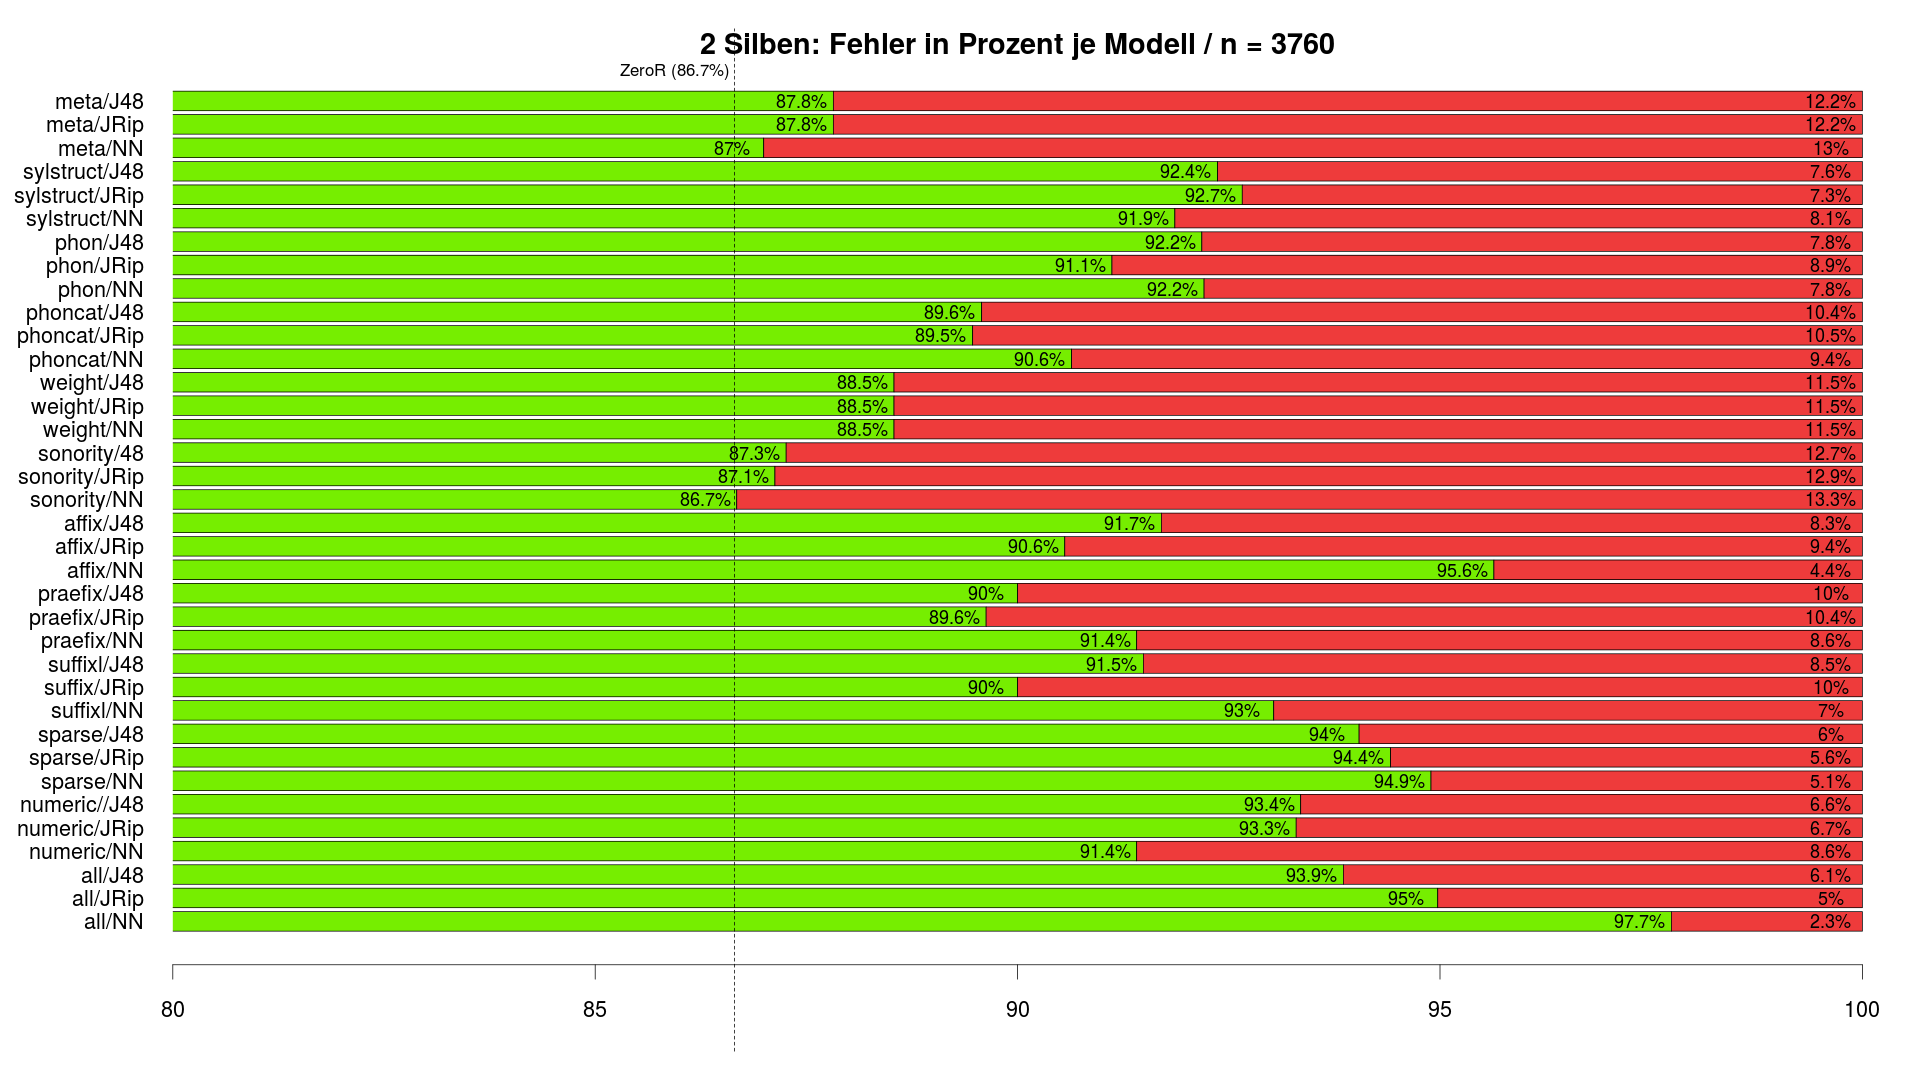
\includegraphics[width=12cm]{figures/basicstats/2syl-basicstats.png}}\end{center}
\begin{center}{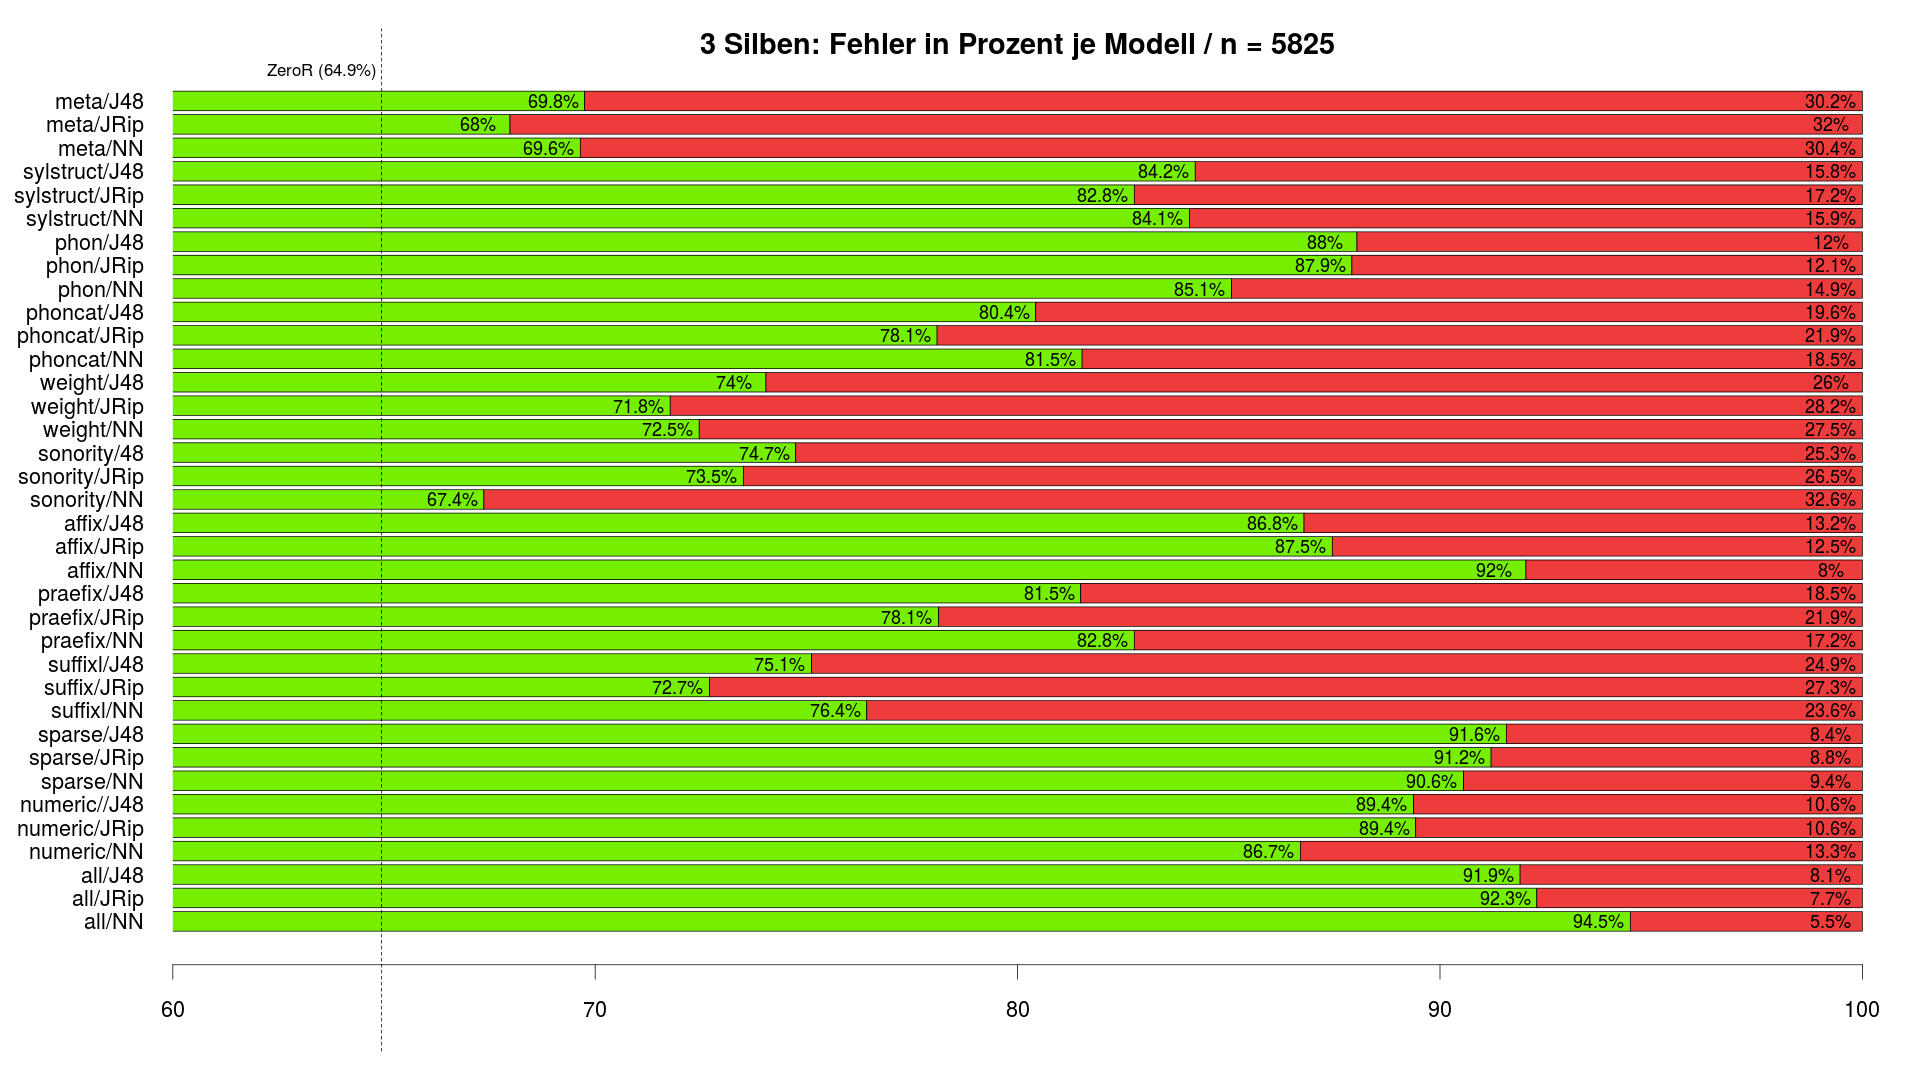
\includegraphics[width=12cm]{figures/basicstats/3syl-basicstats.png}}\end{center}
\begin{center}{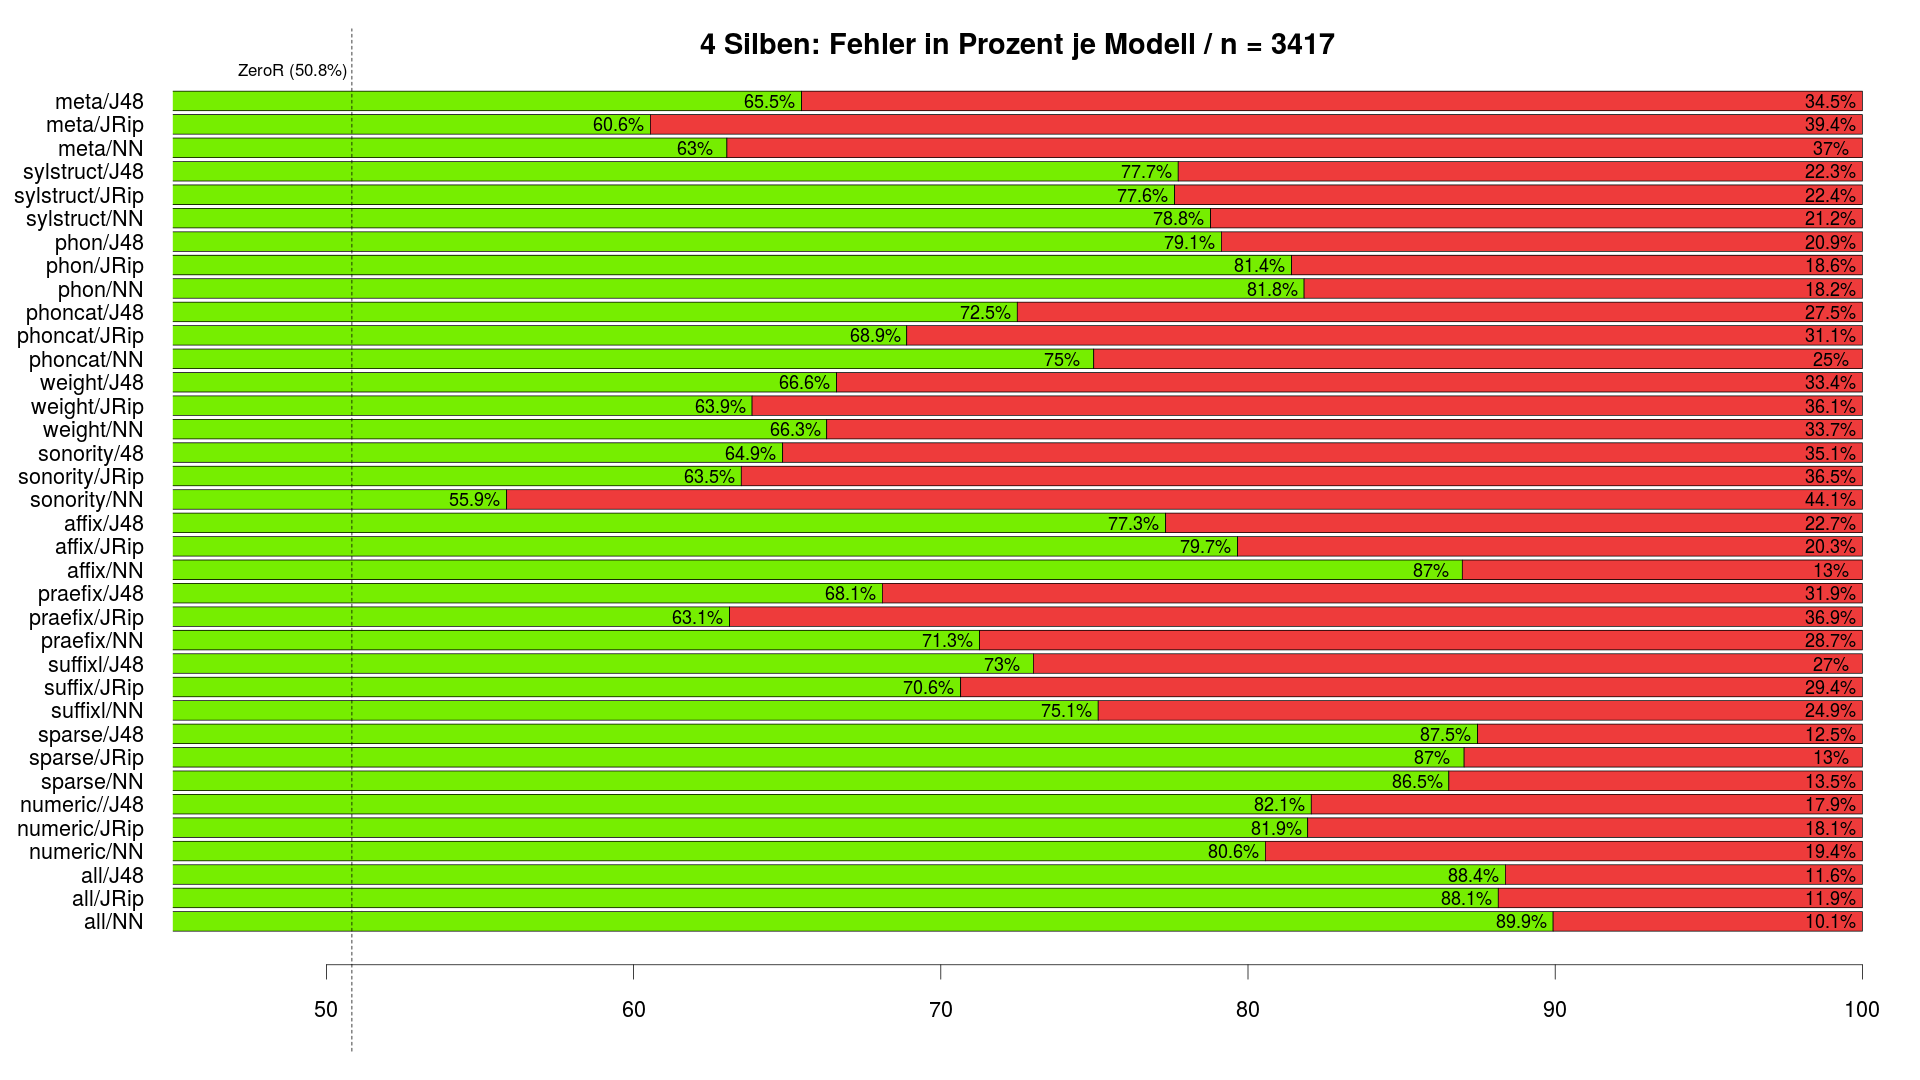
\includegraphics[width=12cm]{figures/basicstats/4syl-basicstats.png}}\end{center}
\begin{center}{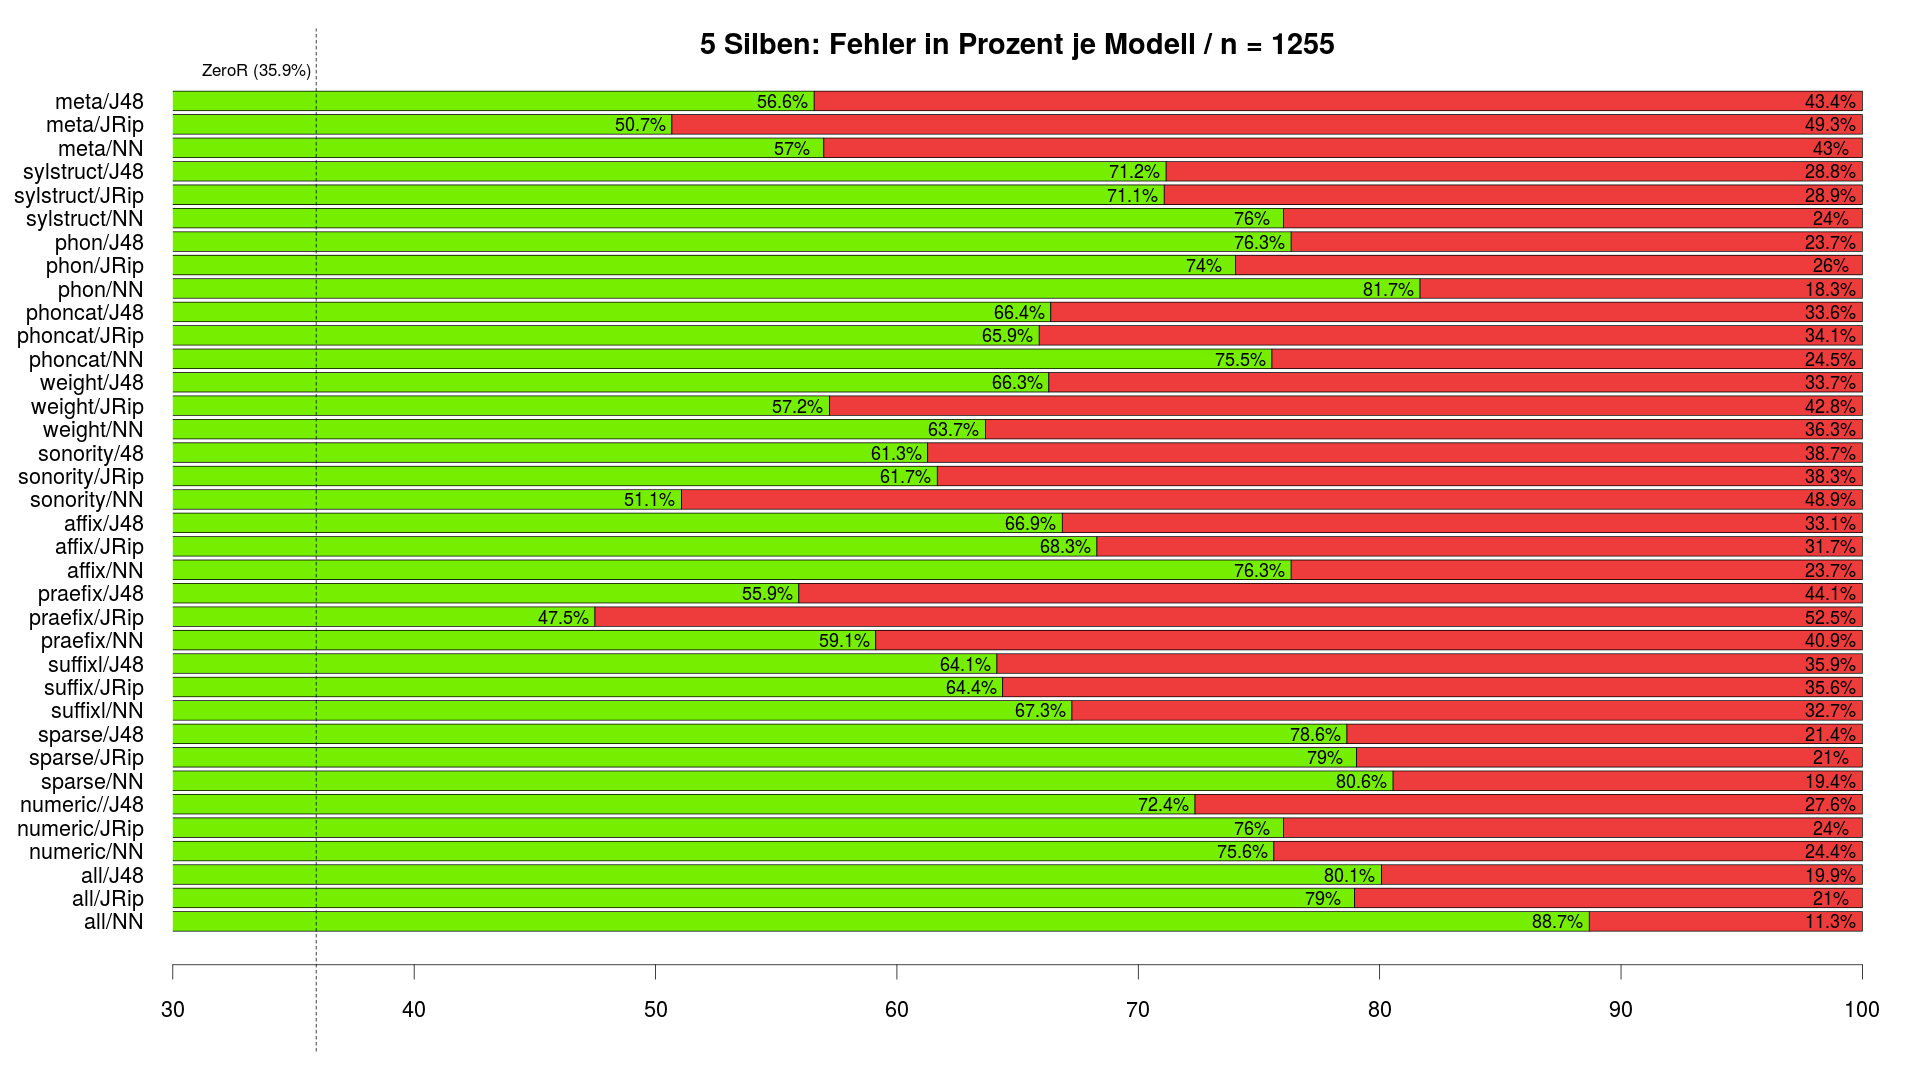
\includegraphics[width=12cm]{figures/basicstats/5syl-basicstats.png}}\end{center}
\begin{center}{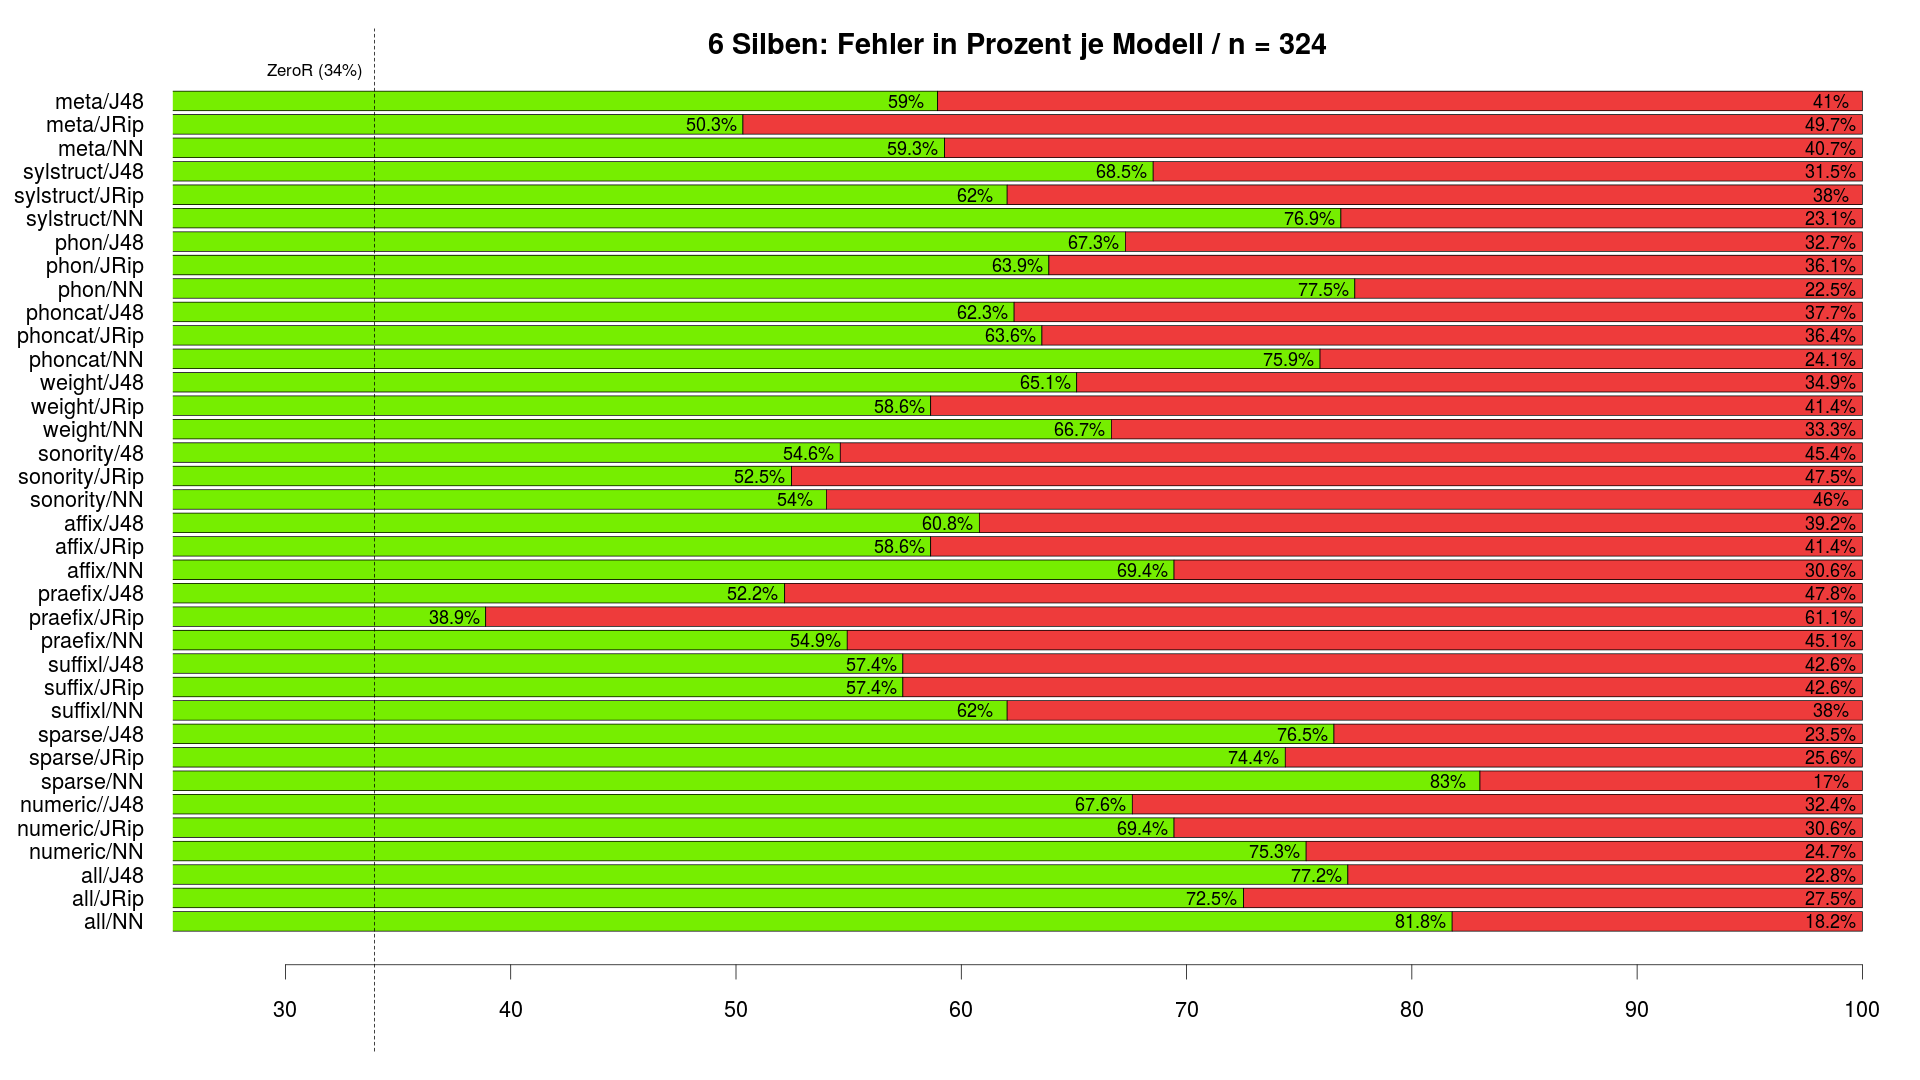
\includegraphics[width=12cm]{figures/basicstats/6syl-basicstats.png}}\end{center}
\begin{center}{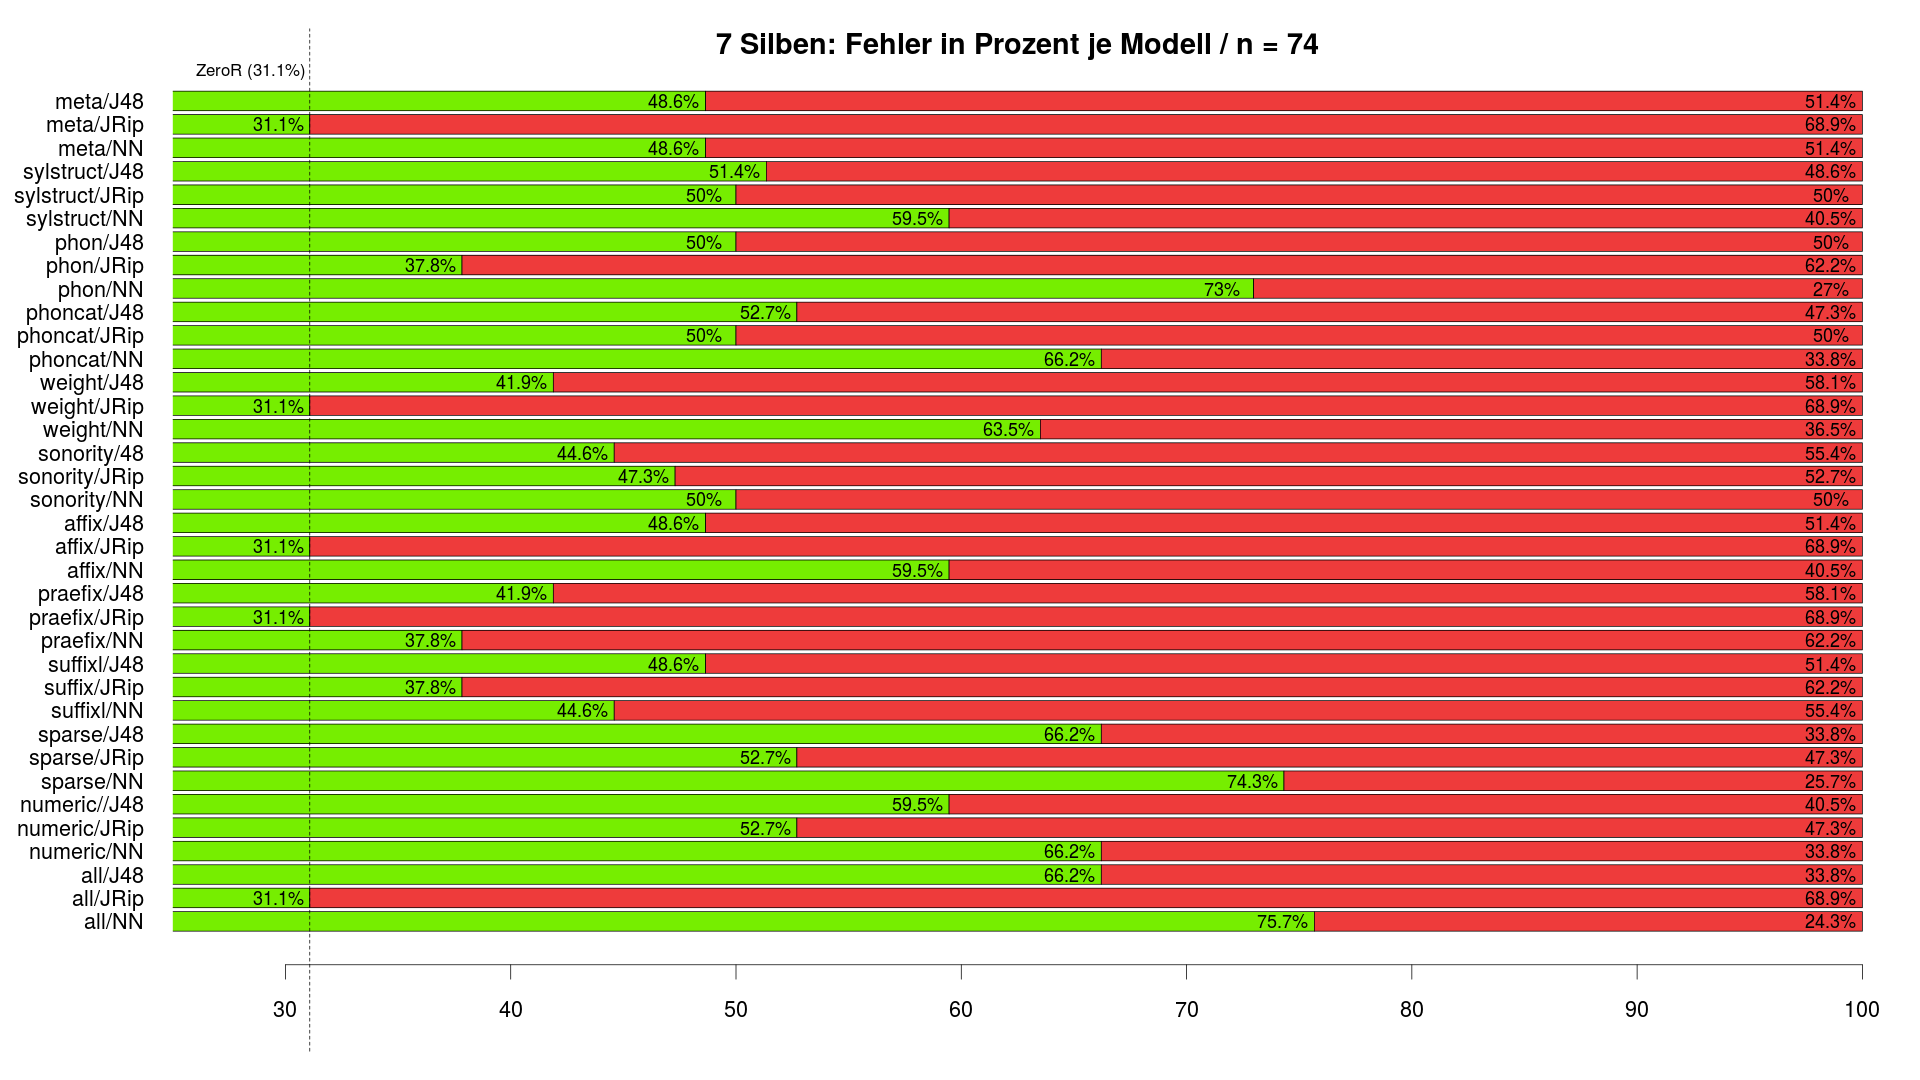
\includegraphics[width=12cm]{figures/basicstats/7syl-basicstats.png}}\end{center}
\newpage

%\section{Einfluss der Features}
\begin{figure}[!p]
    \begin{floatrow}
        \ffigbox{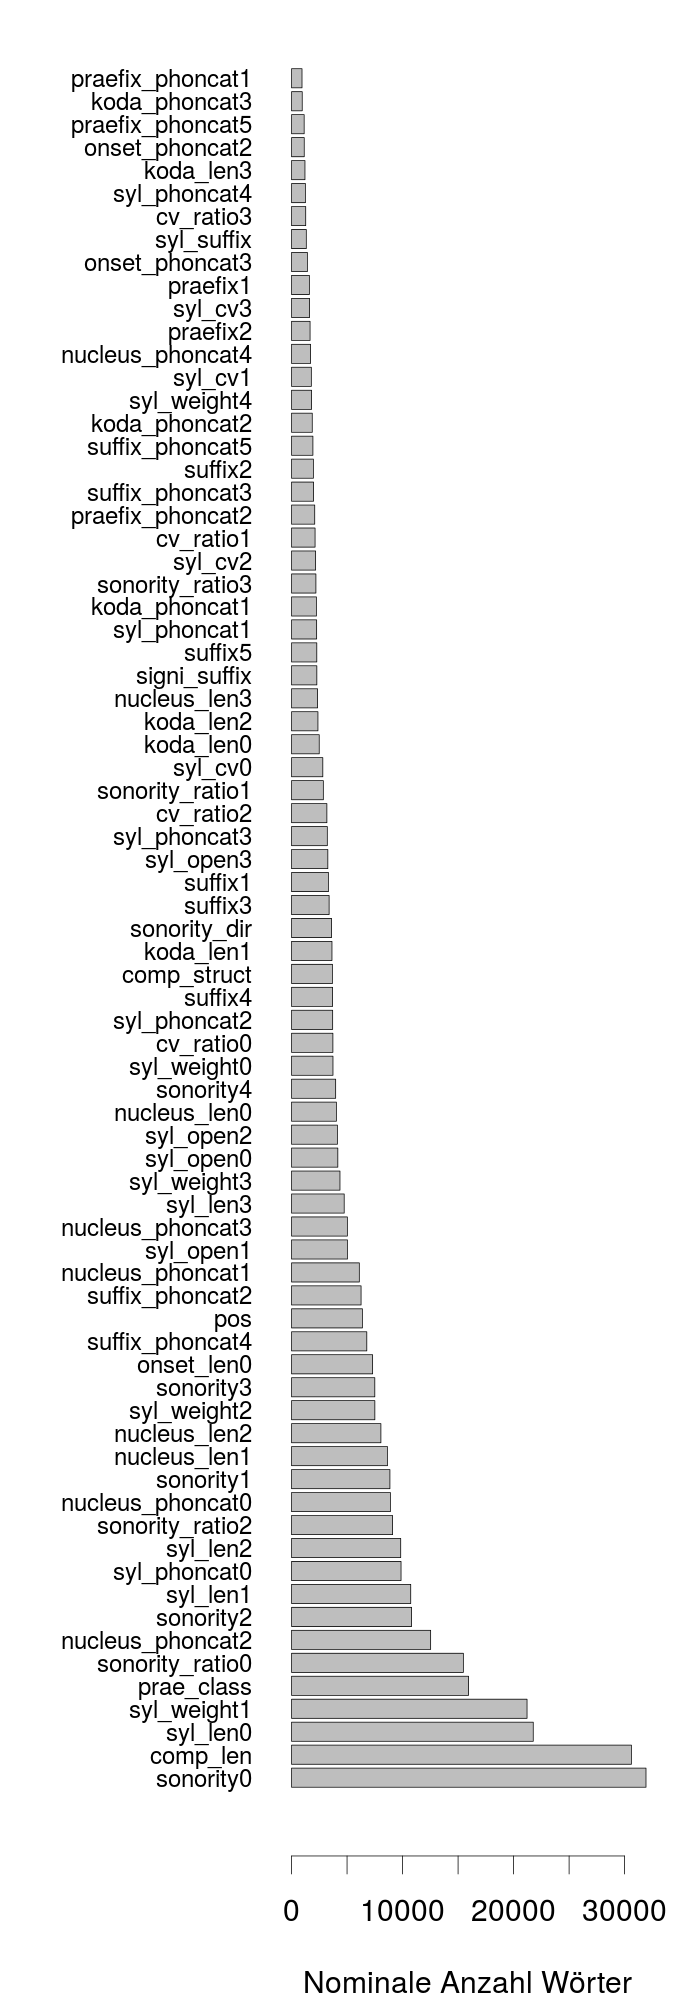
\includegraphics[scale = 0.27]{figures/features/jrip_feature_influence.png}} {
            \caption{75 häufigste Features}
            \label{figure:jrip_feature_influence}
        }
        \ffigbox{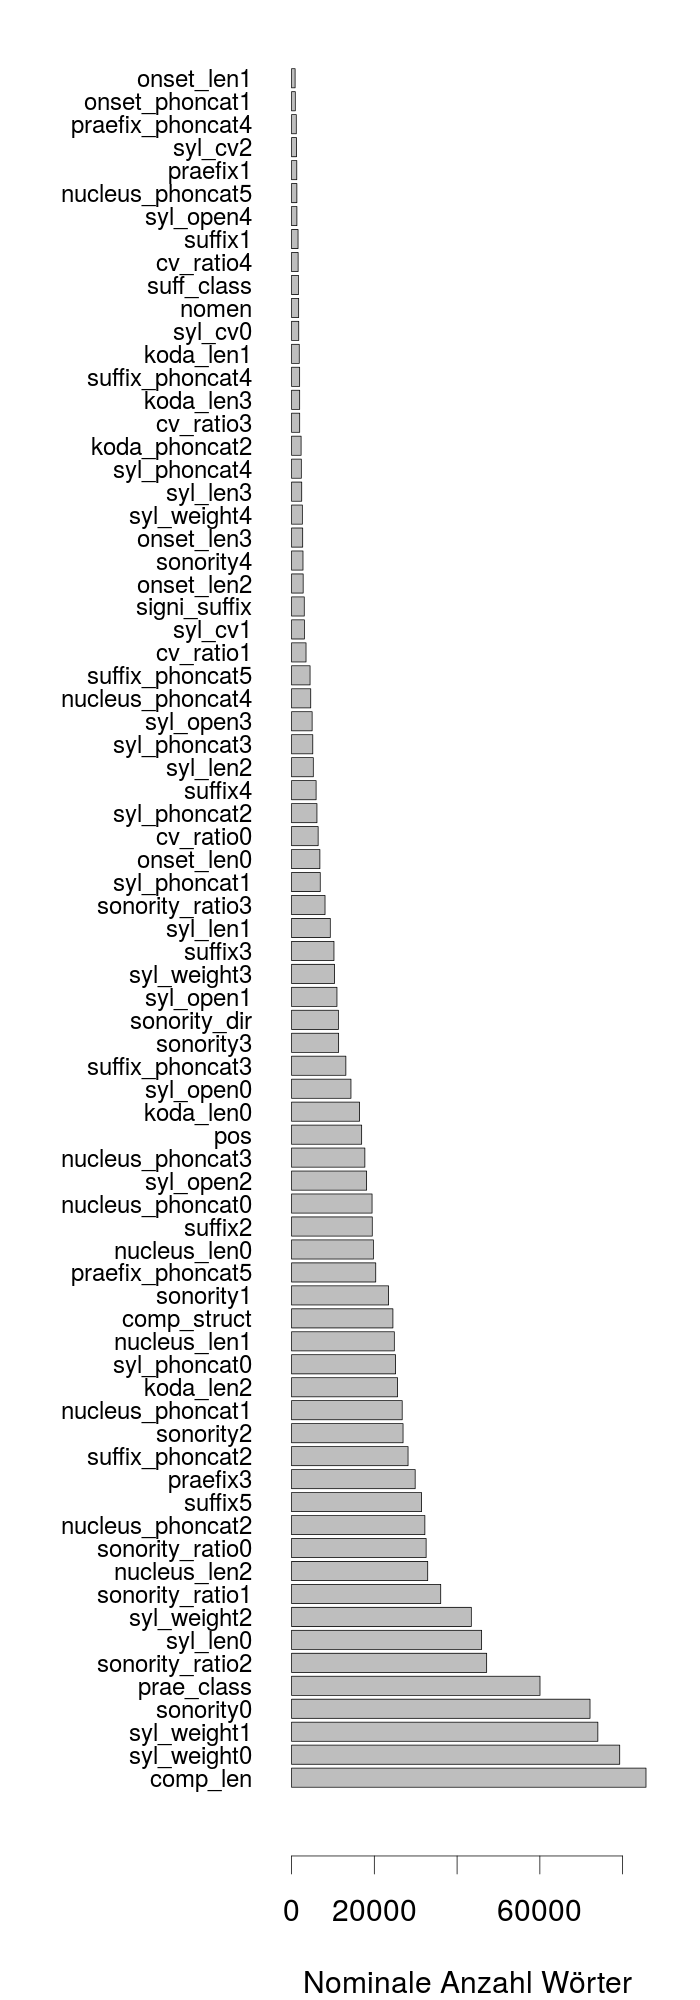
\includegraphics[scale = 0.27]{figures/features/j48_feature_influence.png}} {
            \caption{75 häufigste Features}
            \label{figure:j48_feature_influence}
        }
    \end{floatrow}
\end{figure}

%\section{Beispielregeln von JRip}
\begin{table}
\centering
\tiny
\caption{Die 50 einflussreichsten JRip-Regeln.}
\label{table:jrip_rules_examples}
\begin{tabular}{|p{8cm}l|ll|ll|}\hline
{\bf Regel} & {\bf Klasse} & {\bf TP} & {\bf FP} & {\bf Silben} & {\bf Featureset} \\\hline\hline
(prae\_class = noacc)                                                                                                                                                                                        & paenultima & 1562 & 1   & 3 & praefix   \\\hline
(prae\_class = noacc)                                                                                                                                                                                        & paenultima & 1561 & 1   & 3 & affix     \\\hline
(prae\_class = noacc)                                                                                                                                                                                        & paenultima & 1560 & 1   & 3 & all       \\\hline
(prae\_class = noacc)                                                                                                                                                                                        & paenultima & 1559 & 1   & 3 & sparse    \\\hline
(nucleus\_phoncat0 = K) and (syl\_phoncat0 = CK) and (nucleus\_phoncat2 = K)                                                                                                                                 & paenultima & 1137 & 271 & 3 & phoncat   \\\hline
(nucleus\_phoncat0 = K) and (syl\_phoncat2 = CKC) and (syl\_phoncat0 = CKC)                                                                                                                                  & paenultima & 1069 & 388 & 3 & phoncat   \\\hline
(syl\_cv0 = CVC) and (nucleus\_len1 \textgreater= 2) and (syl\_len0 \textless= 3)                                                                                                                            & paenultima & 896  & 175 & 3 & sylstruct \\\hline
(nucleus\_phoncat0 = K) and (syl\_weight1 = light) and (sonority0 \textless= 11) and (sonority0 \textgreater= 10) and (syl\_phoncat0 = CKC) and (sonority0 \textgreater= 11)                                 & paenultima & 877  & 95  & 3 & phon      \\\hline
(sonority0 \textless= 11) and (sonority\_ratio0 \textless= 3) and (sonority\_ratio0 \textgreater= 3) and (sonority0 \textgreater= 11) and (sonority1 \textgreater= 11) and (sonority2 \textgreater= 10)      & paenultima & 738  & 217 & 3 & sonority  \\\hline
(comp\_len \textless= 1) and (cv\_ratio0 \textgreater= 2) and (syl\_len0 \textless= 3) and (sonority\_ratio0 \textless= 3) and (nucleus\_len1 \textgreater= 2)                                               & paenultima & 729  & 45  & 3 & numeric   \\\hline
(syl\_weight0 = schwa)                                                                                                                                                                                       & paenultima & 721  & 0   & 3 & weight    \\\hline
(nucleus\_phoncat0 = K) and (syl\_open0 = o)                                                                                                                                                                 & paenultima & 716  & 0   & 3 & phon      \\\hline
(nucleus\_len0 \textless= 1) and (syl\_len0 \textless= 3) and (syl\_cv0 = CV)                                                                                                                                & paenultima & 713  & 0   & 3 & sylstruct \\\hline
(comp\_len \textless= 1) and (sonority\_ratio0 \textless= 3) and (koda\_len0 \textless= 0) and (nucleus\_len0 \textless= 1)                                                                                  & paenultima & 664  & 0   & 3 & numeric   \\\hline
(comp\_len \textless= 1) and (nucleus\_len2 \textgreater= 2) and (cv\_ratio1 \textless= 0)                                                                                                                   & paenultima & 647  & 83  & 4 & numeric   \\\hline
(syl\_len0 \textless= 3) and (nucleus\_len0 \textless= 1) and (syl\_cv2 = CVC) and (syl\_len0 \textgreater= 3) and (koda\_len1 \textgreater= 1)                                                              & paenultima & 637  & 174 & 3 & sylstruct \\\hline
(nucleus\_phoncat3 = L) and (nucleus\_phoncat2 = L)                                                                                                                                                          & paenultima & 610  & 167 & 5 & phoncat   \\\hline
(nucleus\_len2 \textgreater= 2) and (comp\_len \textless= 1) and (signi\_suffix = ø) and (suffix\_phoncat2 = LC) and (syl\_weight1 = light)                                                                  & ultima     & 595  & 56  & 3 & all       \\\hline
(nucleus\_phoncat2 = L) and (nucleus\_phoncat1 = L) and (syl\_phoncat3 = CKC)                                                                                                                                & paenultima & 558  & 71  & 4 & phoncat   \\\hline
(sonority0 \textless= 11) and (sonority\_ratio0 \textless= 3) and (sonority\_ratio0 \textgreater= 3) and (sonority\_ratio2 \textgreater= 4) and (sonority\_dir \textless= 1) and (sonority1 \textgreater= 8) & paenultima & 544  & 204 & 3 & sonority  \\\hline
(nucleus\_len2 \textgreater= 2) and (comp\_len \textless= 1) and (syl\_len1 \textless= 2) and (onset\_len0 \textgreater= 1) and (syl\_len2 \textgreater= 3)                                                  & ultima     & 516  & 44  & 3 & sparse    \\\hline
(nucleus\_len2 \textgreater= 2) and (comp\_len \textless= 1) and (syl\_len1 \textless= 2) and (onset\_len0 \textgreater= 1) and (syl\_len2 \textgreater= 3)                                                  & ultima     & 516  & 44  & 3 & numeric   \\\hline
(nucleus\_phoncat3 = L) and (comp\_len \textless= 1) and (signi\_suffix = ø) and (syl\_len3 \textgreater= 3)                                                                                                 & ultima     & 498  & 56  & 4 & all       \\\hline
(syl\_weight1 = light) and (nucleus\_phoncat2 = L) and (syl\_phoncat4 = CKC)                                                                                                                                 & paenultima & 490  & 86  & 5 & phon     \\\hline
(suffix\_phoncat4 = LCKC) and (suffix4 = eren)                                                                                                                                                                                                              & paenultima     & 477 & 50  & 4 & suffix    \\\hline
(nucleus\_phoncat3 = L) and (comp\_len \textless= 1) and (syl\_len2 \textless= 2) and (koda\_phoncat3 = C)                                                                                                                                                  & ultima         & 477 & 38  & 4 & sparse    \\\hline
(nucleus\_phoncat1 = L) and (nucleus\_phoncat2 = L) and (onset\_phoncat3 = C) and (syl\_open1 = o)                                                                                                                                                          & paenultima     & 463 & 77  & 4 & phon      \\\hline
(syl\_weight1 = light) and (nucleus\_phoncat2 = L) and (sonority0 \textless= 10) and (sonority3 \textgreater= 13)                                                                                                                                           & paenultima     & 454 & 44  & 4 & phon      \\\hline
(comp\_len \textless= 1) and (sonority0 \textless= 10) and (sonority0 \textgreater= 10) and (onset\_len0 \textless= 0) and (nucleus\_len0 \textless= 1)                                                                                                     & paenultima     & 450 & 23  & 3 & numeric   \\\hline
(sonority\_ratio0 \textless= 4) and (sonority2 \textgreater= 10) and (sonority\_ratio2 \textless= 4) and (sonority0 \textless= 11)                                                                                                                          & sekunda        & 447 & 197 & 5 & sonority  \\\hline
(comp\_len \textless= 1) and (cv\_ratio0 \textgreater= 2) and (sonority0 \textless= 11) and (sonority0 \textgreater= 11) and (koda\_len1 \textgreater= 1) and (nucleus\_len2 \textless= 1) and (syl\_len0 \textless= 3) and (sonority\_ratio0 \textless= 3) & paenultima     & 435 & 12  & 3 & numeric   \\\hline
(nucleus\_len2 \textgreater= 2) and (syl\_cv1 = CVV) and (koda\_len2 \textgreater= 1)                                                                                                                                                                       & ultima         & 428 & 80  & 3 & sylstruct \\\hline
(suffix\_phoncat4 = LCKC) and (suffix5 = ieren) and (prae\_class = ø)                                                                                                                                                                                       & paenultima     & 426 & 4   & 4 & affix     \\\hline
(sonority\_dir \textgreater= 1) and (sonority\_ratio2 \textgreater= 4) and (sonority3 \textgreater= 13) and (sonority3 \textless= 13)                                                                                                                       & paenultima     & 425 & 106 & 4 & sonority  \\\hline
(syl\_weight3 = light) and (syl\_open2 = o) and (syl\_weight2 = light) and (syl\_weight1 = light) and (syl\_open0 = o)                                                                                                                                      & ultima         & 416 & 207 & 4 & weight    \\\hline
(syl\_len0 \textless= 2) and (nucleus\_len1 \textgreater= 2) and (onset\_len0 \textgreater= 1) and (onset\_len2 \textgreater= 1)                                                                                                                            & paenultima     & 412 & 113 & 3 & numeric   \\\hline
(comp\_len \textless= 1) and (sonority0 \textless= 10) and (nucleus\_phoncat2 = L) and (syl\_weight1 = light) and (sonority1 \textless= 10) and (onset\_phoncat3 = C)                                                                                       & paenultima     & 398 & 37  & 4 & all       \\\hline
(prae\_class = noacc)                                                                                                                                                                                                                                       & antepaenultima & 392 & 2   & 4 & sparse    \\\hline
(prae\_class = noacc)                                                                                                                                                                                                                                       & antepaenultima & 392 & 2   & 4 & praefix   \\\hline
(prae\_class = noacc)                                                                                                                                                                                                                                       & antepaenultima & 392 & 2   & 4 & all       \\\hline
(prae\_class = noacc)                                                                                                                                                                                                                                       & antepaenultima & 390 & 2   & 4 & affix     \\\hline
(syl\_suffix = ø) and (comp\_len \textless= 1) and (syl\_weight2 = heavy) and (syl\_weight1 = light)                                                                                                                                                        & ultima         & 382 & 74  & 3 & all       \\\hline
(sonority0 \textless= 11) and (syl\_weight1 = light) and (syl\_open0 = o) and (syl\_phoncat0 = CL) and (onset\_phoncat2 = C) and (nucleus\_phoncat2 = K)                                                                                                    & paenultima     & 378 & 103 & 3 & phon      \\\hline
(sonority0 \textless= 10) and (syl\_weight1 = light) and (sonority0 \textgreater= 10) and (nucleus\_phoncat0 = K) and (sonority\_ratio0 \textgreater= 5)                                                                                                    & paenultima     & 370 & 31  & 3 & phon      \\\hline
(syl\_len0 \textless= 2) and (nucleus\_len2 \textgreater= 2) and (nucleus\_len1 \textgreater= 2) and (syl\_cv3 = CVC) and (syl\_len1 \textless= 3)                                                                                                          & paenultima     & 364 & 39  & 4 & sylstruct \\\hline
(nucleus\_phoncat2 = L) and (syl\_phoncat1 = CL) and (koda\_phoncat2 = C)                                                                                                                                                                                   & ultima         & 359 & 60  & 3 & phoncat   \\\hline
(comp\_len \textless= 1) and (sonority0 \textless= 10) and (syl\_weight1 = light) and (prae\_class = ø) and (syl\_weight3 = schwa)                                                                                                                          & paenultima     & 359 & 50  & 4 & sparse    \\\hline
\end{tabular}
\end{table}
\begin{landscape}
\begin{table}[p]
\centering
\tiny
\caption{Drei Beispiele für die Wörter \textit{knifflig, ruecklings} und \textit{trennen} aus dem Trainingsset der Zweisilber.}
\label{table:data_example}
\begin{tabular}{|p{2cm}|p{2cm}|p{2cm}|p{2cm}|p{2cm}|p{1.5cm}|p{1.5cm}|p{1.5cm}|p{1.8cm}|p{1.8cm}|}
\hline
{\bf syl\_suffix}       & {\bf signi\_suffix}     & {\bf suffix1}           & {\bf suffix2}           & {\bf suffix3}           & {\bf suffix4}       & {\bf suffix5}       & {\bf suffix\_phoncat1} & {\bf suffix\_phoncat2} & {\bf suffix\_phoncat3} \\\hline
ø                       & ø                       & g                       & ig                      & lig                     & ø                   & ø                   & C                      & KC                     & CKC                    \\
ø                       & ø                       & s                       & ø                       & ø                       & ø                   & ø                   & C                      & CC                     & KCC                    \\
nen                     & ø                       & n                       & en                      & nen                     & ø                   & ø                   & C                      & KC                     & CKC                    \\\hline
\hline
{\bf suffix\_phoncat4}  & {\bf suffix\_phoncat5}  & {\bf suff\_class}       & {\bf syl\_praefix}      & {\bf signi\_praefix}    & {\bf praefix1}      & {\bf praefix2}      & {\bf praefix3}         & {\bf praefix4}         & {\bf praefix5}         \\
CCKC                    & KCCKC                   & ø                       & ø                       & ø                       & k                   & kn                  & ø                      & ø                      & ø                      \\
CKCC                    & CCKCC                   & ø                       & ø                       & ø                       & r                   & ru                  & ø                      & ø                      & ø                      \\
KCKC                    & CKCKC                   & ø                       & ø                       & ø                       & t                   & tr                  & ø                      & ø                      & ø                      \\\hline
\hline
{\bf praefix\_phoncat1} & {\bf praefix\_phoncat2} & {\bf praefix\_phoncat3} & {\bf praefix\_phoncat4} & {\bf praefix\_phoncat5} & {\bf prae\_class}   & {\bf sonority0}     & {\bf sonority1}        & {\bf sonority\_ratio0} & {\bf sonority\_ratio1} \\
C                       & CC                      & CCK                     & CCKC                    & CCKCC                   & ø                   & 13                  & 13                     & 3                      & 4                      \\
C                       & CK                      & CKC                     & CKCC                    & CKCCK                   & ø                   & 13                  & 16                     & 4                      & 4                      \\
C                       & CC                      & CCK                     & CCKC                    & CCKCK                   & ø                   & 11                  & 12                     & 3                      & 4                      \\\hline
\hline
{\bf sonority\_dir}     & {\bf syl\_weight0}      & {\bf syl\_weight1}      & {\bf syl\_open0}        & {\bf syl\_open1}        & {\bf syl\_phoncat0} & {\bf syl\_phoncat1} & {\bf onset\_phoncat0}  & {\bf onset\_phoncat1}  & {\bf koda\_phoncat0}   \\
0                       & light                   & light                   & c                       & c                       & CCKC                & CKC                 & CC                     & C                      & C                      \\
2                       & light                   & heavy                   & c                       & c                       & CKC                 & CKCC                & C                      & C                      & C                      \\
1                       & light                   & schwa                   & c                       & c                       & CCK                 & CKC                 & CC                     & C                      & ø                      \\\hline
\hline
{\bf koda\_phoncat1}    & {\bf nucleus\_phoncat0} & {\bf nucleus\_phoncat1} & {\bf syl\_len0}         & {\bf syl\_len1}         & {\bf koda\_len0}    & {\bf koda\_len1}    & {\bf onset\_len0}      & {\bf onset\_len1}      & {\bf nucleus\_len0}    \\
C                       & K                       & K                       & 4                       & 4                       & 1                   & 1                   & 2                      & 1                      & 1                      \\
CC                      & K                       & K                       & 4                       & 5                       & 1                   & 2                   & 1                      & 1                      & 1                      \\
C                       & K                       & K                       & 4                       & 3                       & 1                   & 1                   & 2                      & 1                      & 1                      \\\hline
\hline
{\bf nucleus\_len1}     & {\bf syl\_cv0}          & {\bf syl\_cv1}          & {\bf cv\_ratio0}        & {\bf cv\_ratio1}        & {\bf pos}           & {\bf comp\_struct}  & {\bf nomen}            & {\bf comp\_len}        & {\bf stress\_class}    \\
1                       & CCVC                    & CVC                     & 3                       & 2                       & A                   & V                   & F                      & 1                      & paenultima             \\
1                       & CVC                     & CVCC                    & 2                       & 3                       & ADV                 & N                   & F                      & 1                      & paenultima             \\
1                       & CCVC                    & CVC                     & 3                       & 2                       & V                   & V                   & F                      & 1                      & paenultima            \\\hline
\end{tabular}
\end{table}
\end{landscape}

%%%%%%%%%%%%%%%%%%%%%

%\begin{landscape}
%\section{Vergleich der Modelle}

%\begin{center}{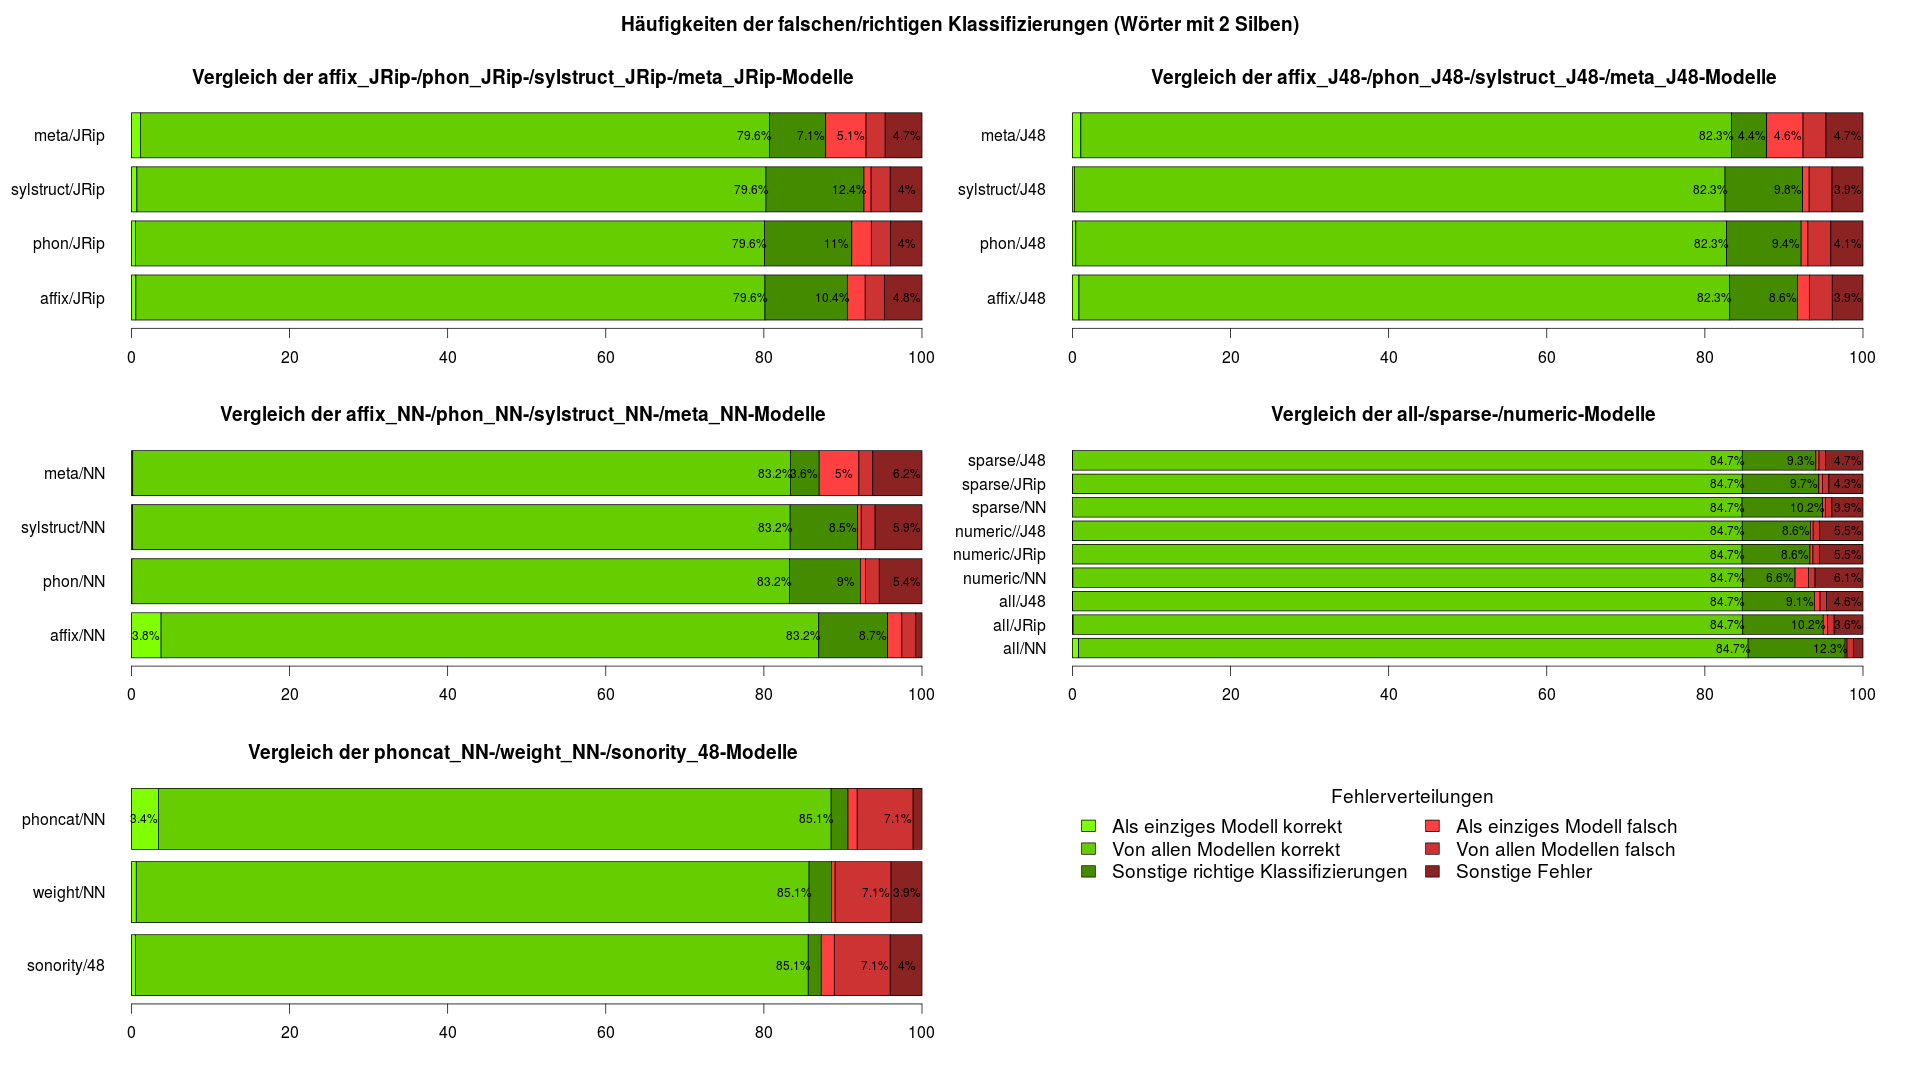
\includegraphics[width=22cm]{figures/compare/2syl.png}}\end{center}
%\begin{center}{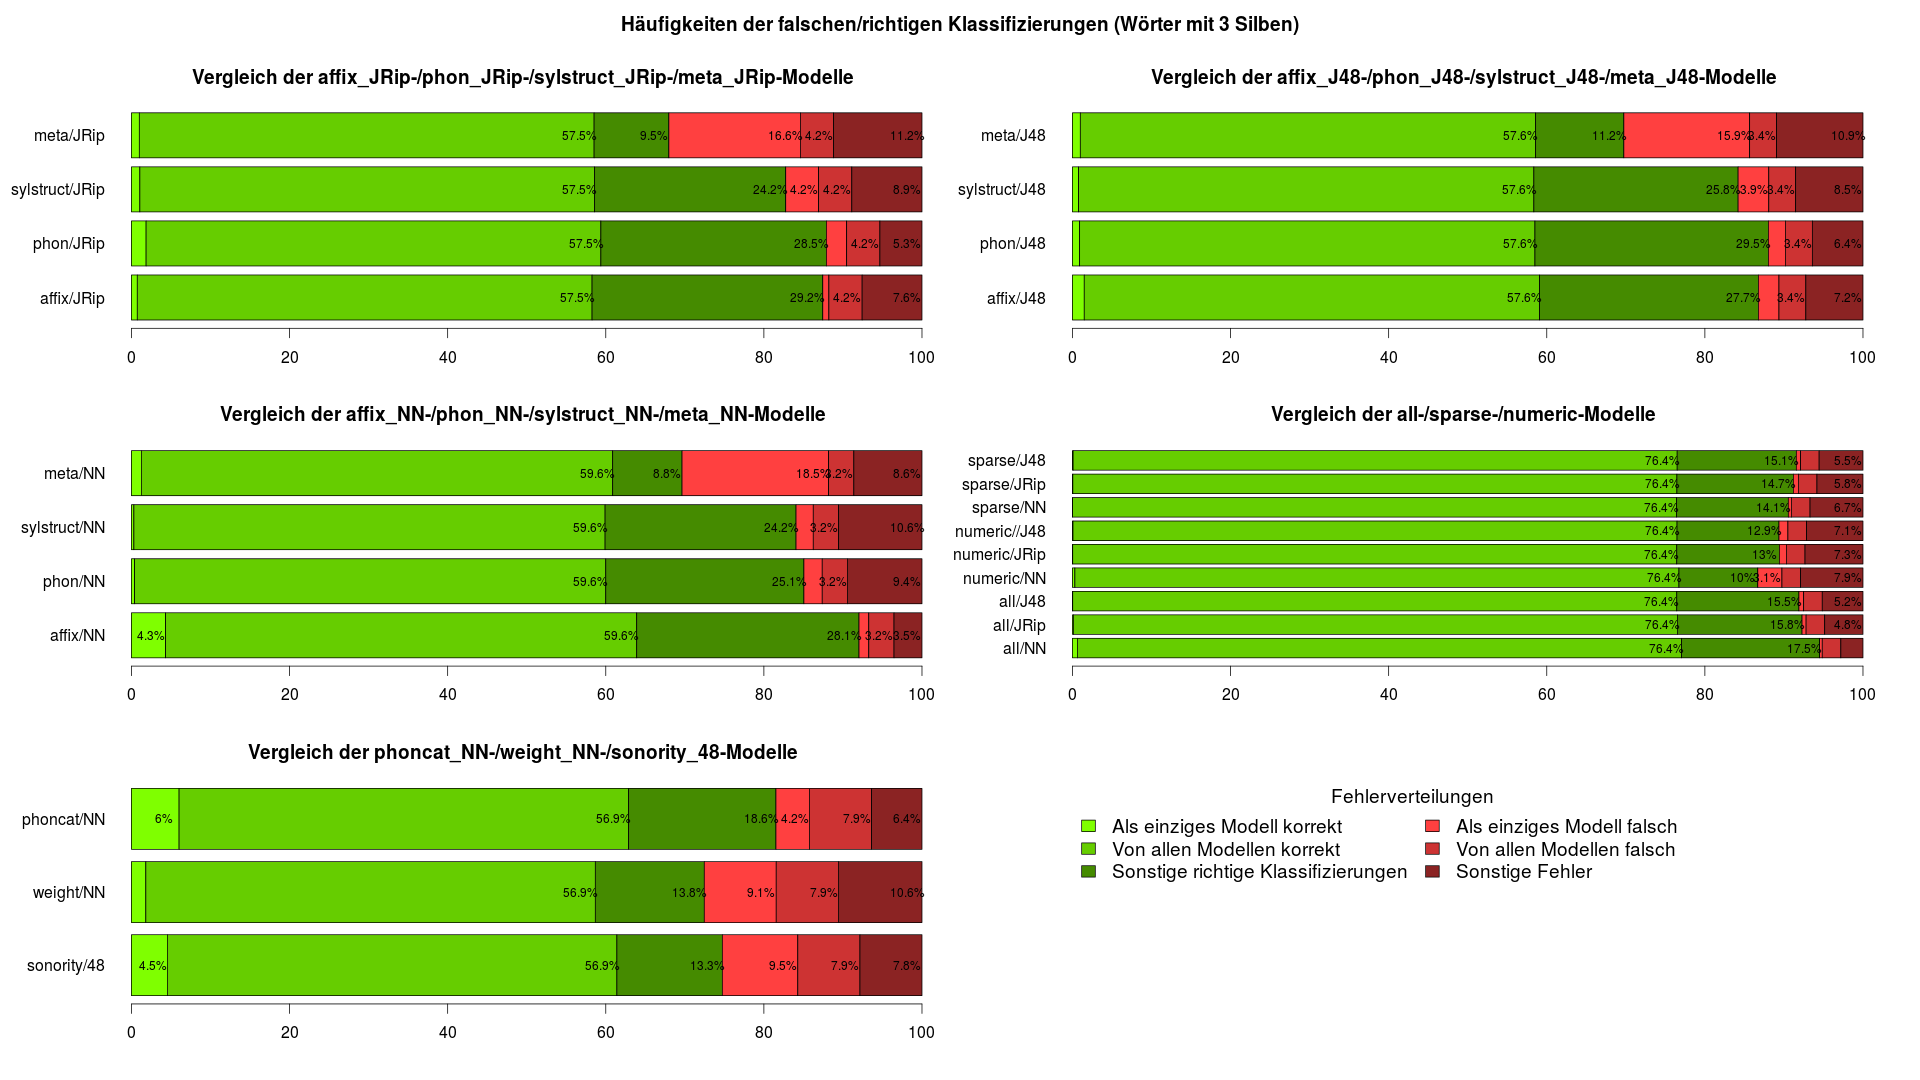
\includegraphics[width=22cm]{figures/compare/3syl.png}}\end{center}
%\begin{center}{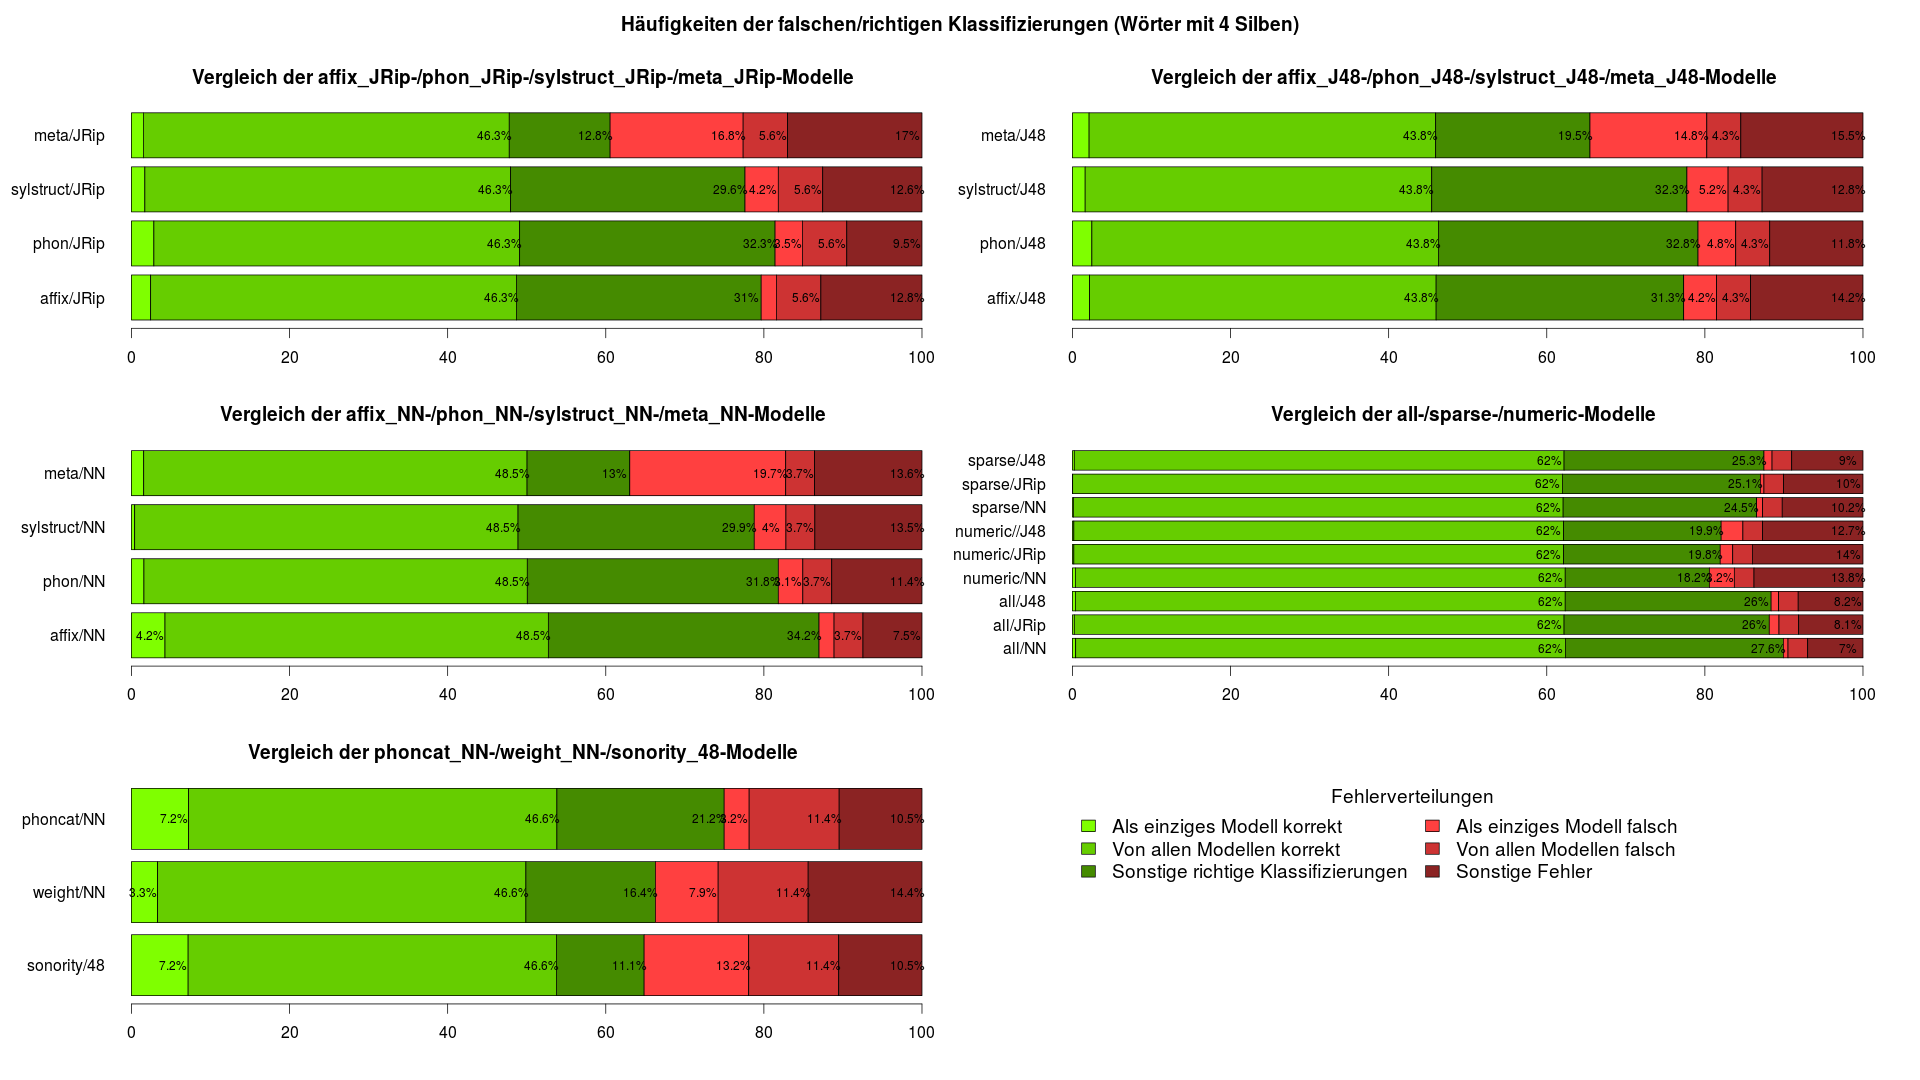
\includegraphics[width=22cm]{figures/compare/4syl.png}}\end{center}
%\begin{center}{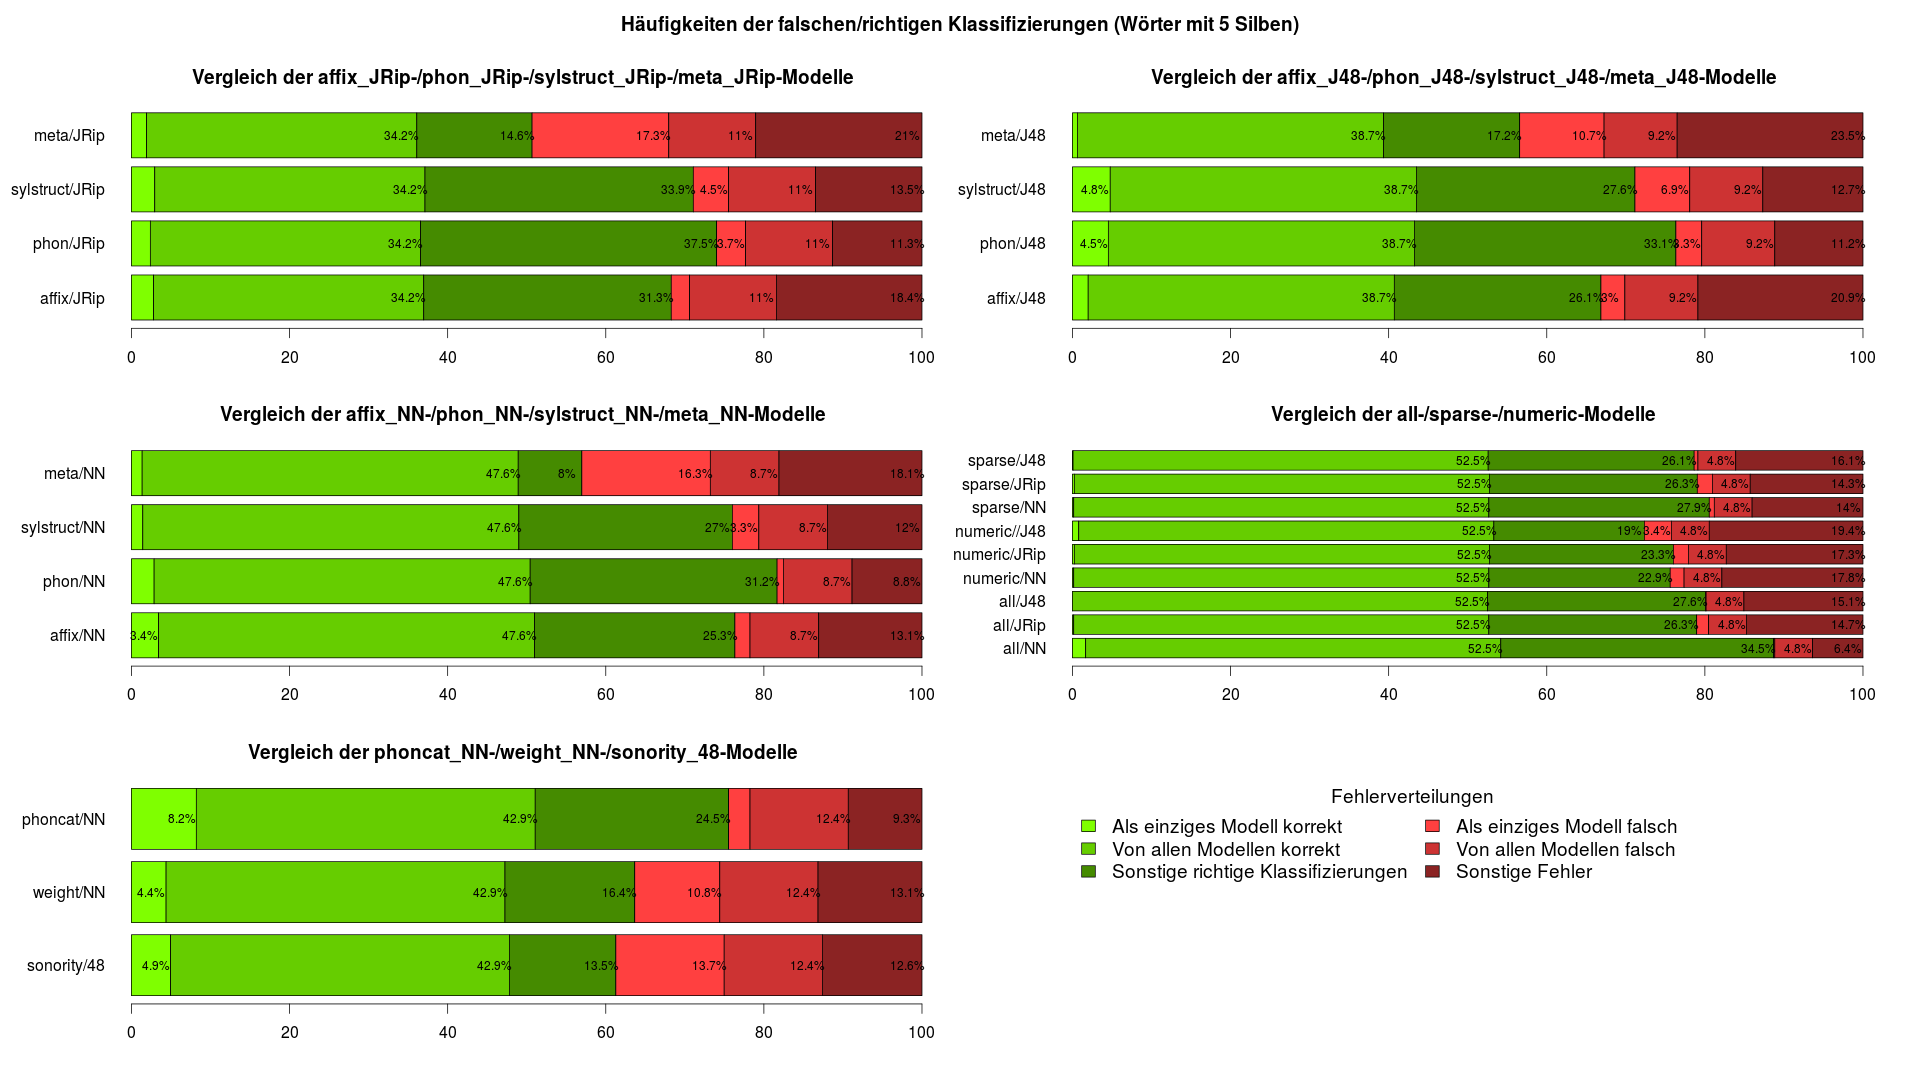
\includegraphics[width=22cm]{figures/compare/5syl.png}}\end{center}
%\begin{center}{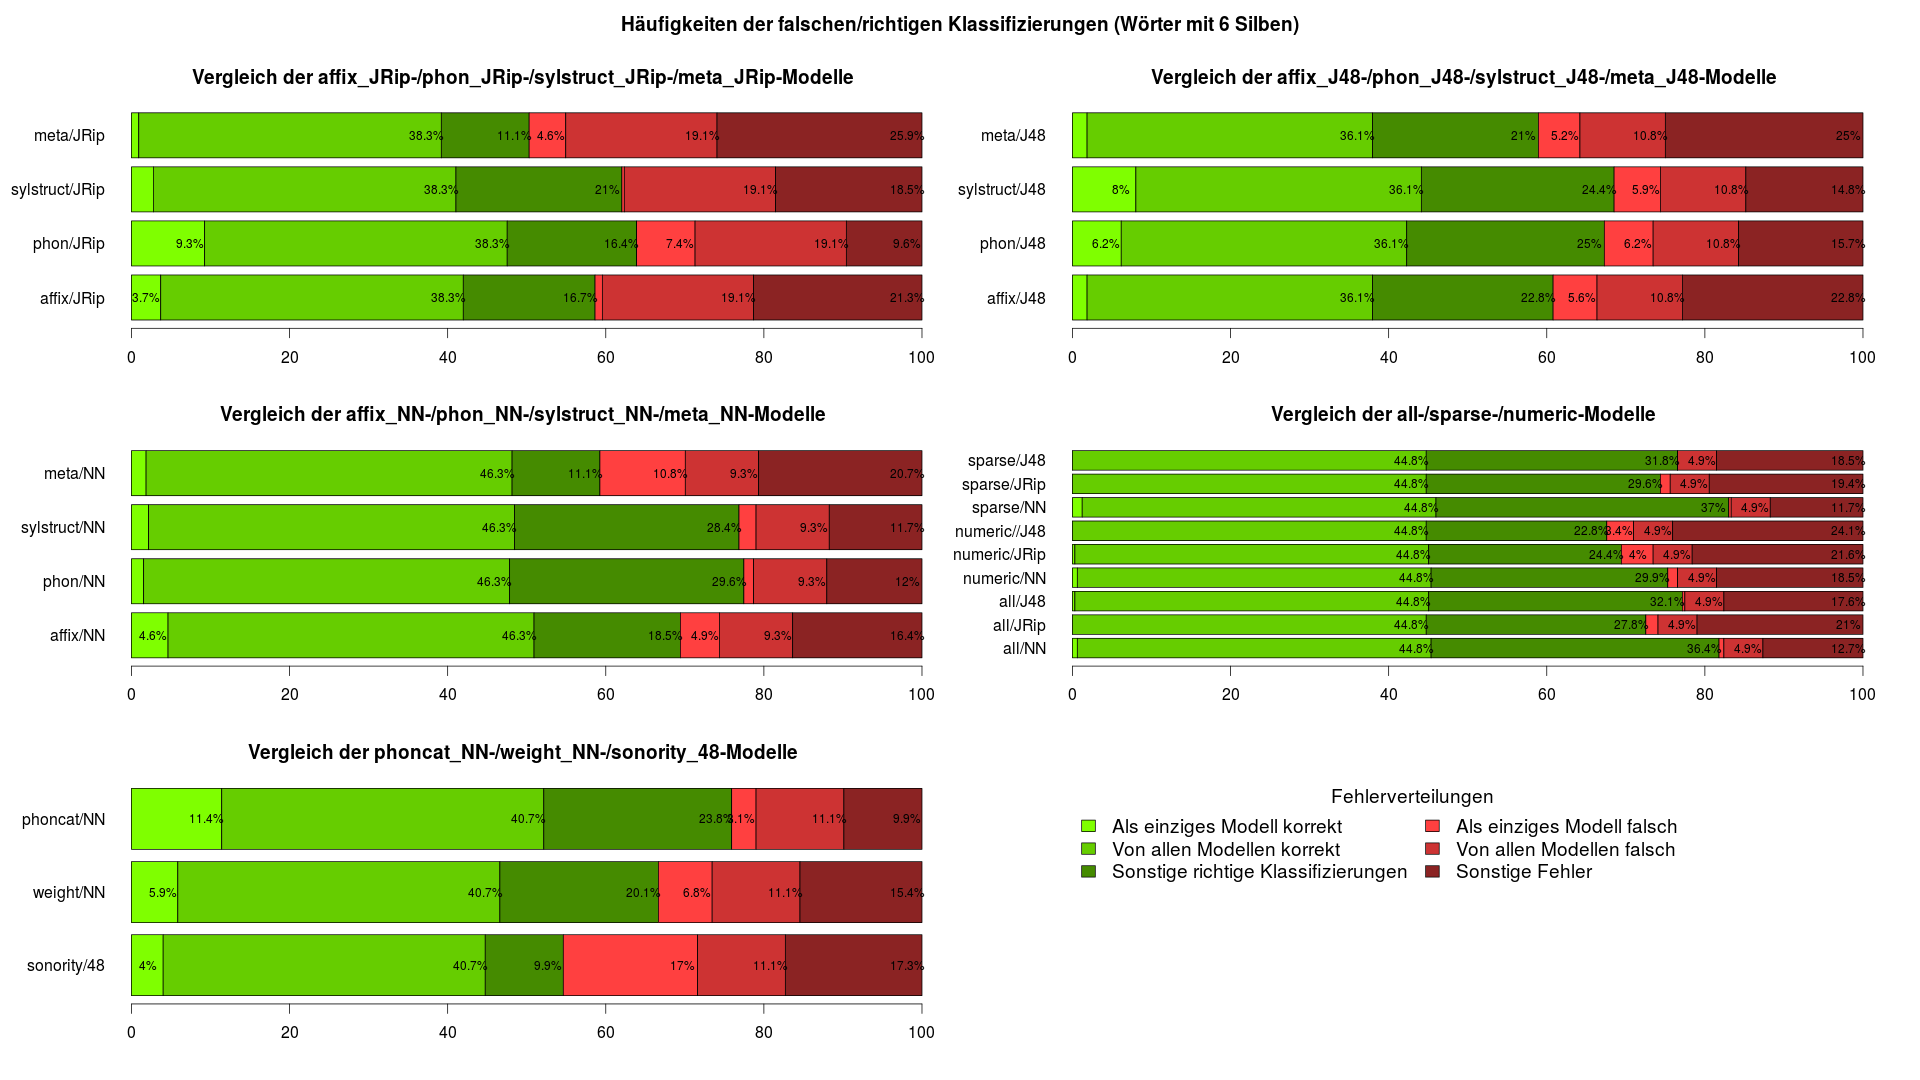
\includegraphics[width=22cm]{figures/compare/6syl.png}}\end{center}
%\begin{center}{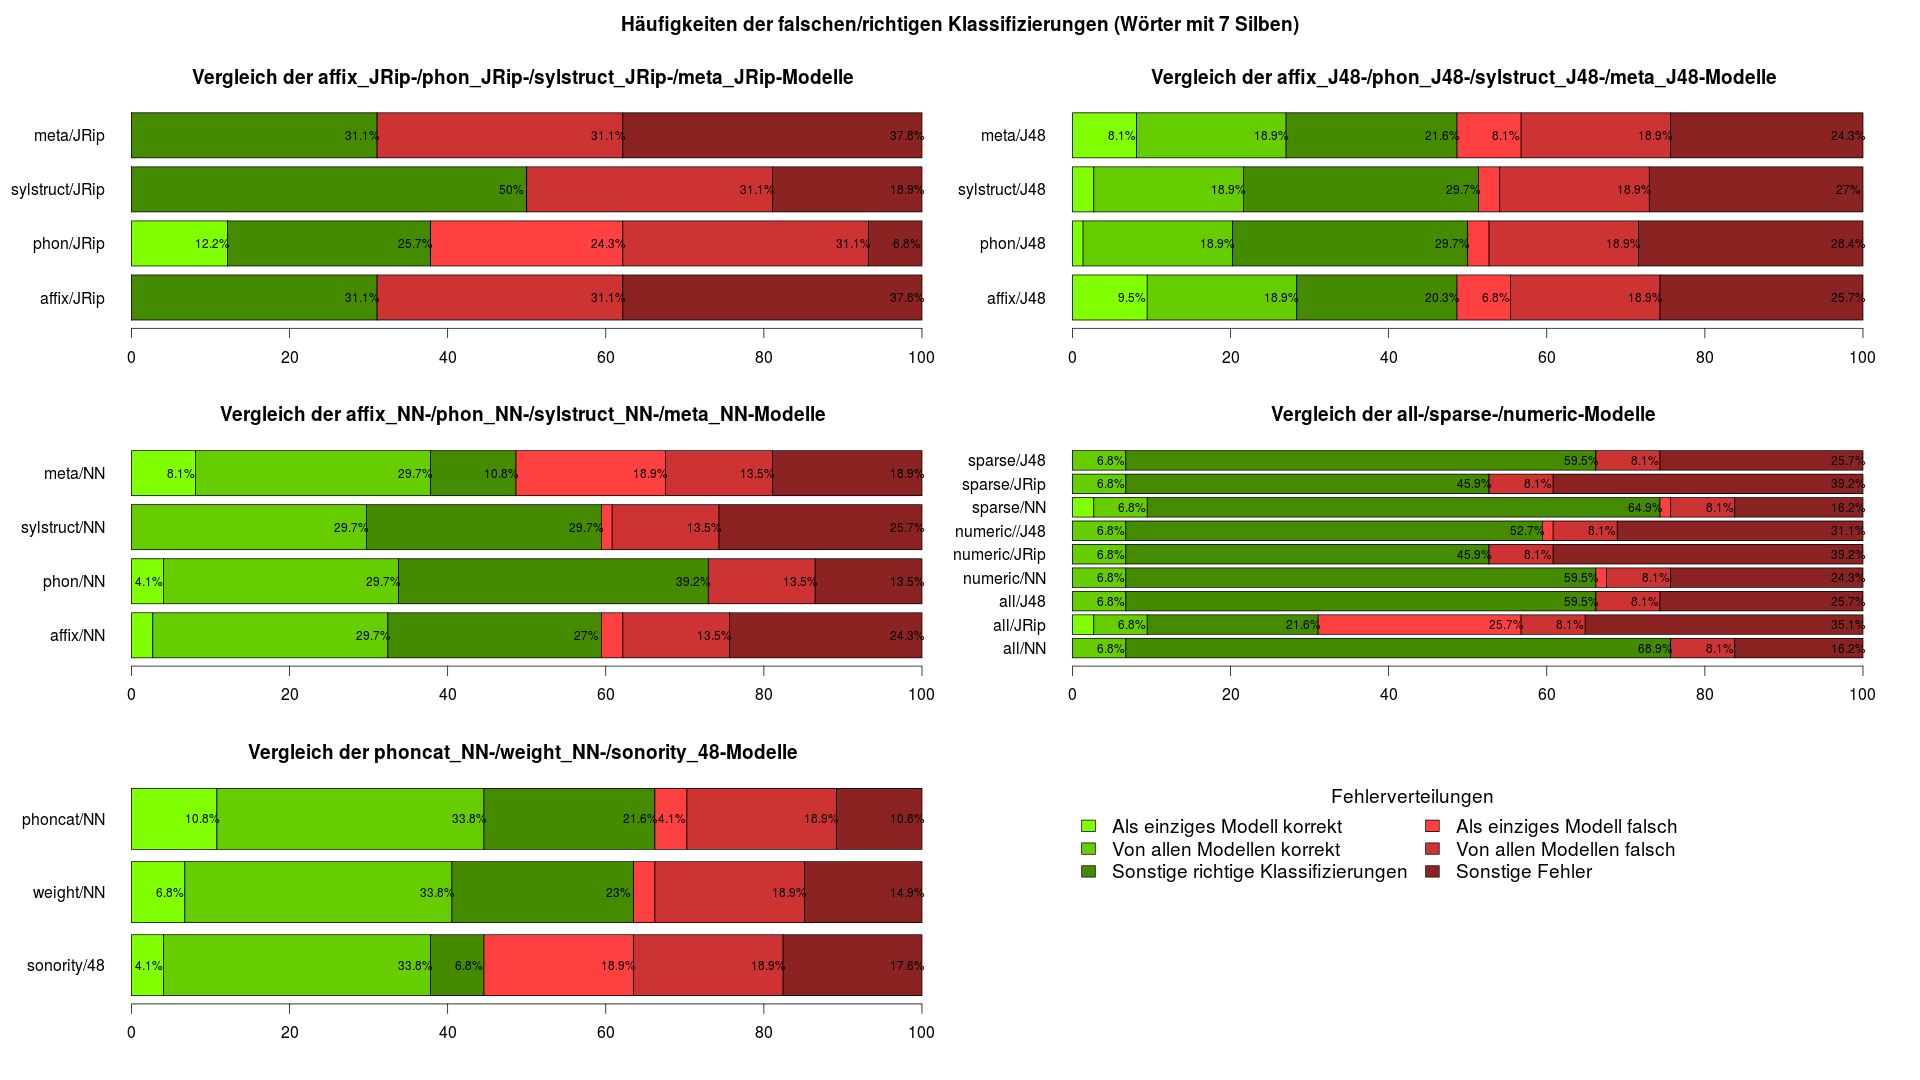
\includegraphics[width=22cm]{figures/compare/7syl.png}}\end{center}
%\end{landscape}

%\cleardoublepage


%%%%%%%%%%%%%%%%%%%%%%%%%%%%%%%%%%%%%%%%%%%%%%%%%%%%%%%%%%%%%%%%%%%%%%%%%%%%%
%%% Bibliographie
%%%%%%%%%%%%%%%%%%%%%%%%%%%%%%%%%%%%%%%%%%%%%%%%%%%%%%%%%%%%%%%%%%%%%%%%%%%%%

\addcontentsline{toc}{chapter}{Literaturverzeichnis}

\bibliographystyle{alpha}
\bibliography{mylit}
%% Obige Anweisung legt fest, dass BibTeX-Datei `mylit.bib' verwendet
%% wird. Hier koennen mehrere Dateinamen mit Kommata getrennt aufgelistet
%% werden.

\cleardoublepage

%%%%%%%%%%%%%%%%%%%%%%%%%%%%%%%%%%%%%%%%%%%%%%%%%%%%%%%%%%%%%%%%%%%%%%%%%%%%%
%%% Erklaerung
%%%%%%%%%%%%%%%%%%%%%%%%%%%%%%%%%%%%%%%%%%%%%%%%%%%%%%%%%%%%%%%%%%%%%%%%%%%%%
\thispagestyle{empty}
\section*{Selbst\"andigkeitserkl\"arung}

Hiermit versichere ich, dass ich die vorliegende Bachelorarbeit 
selbst\"andig und nur mit den angegebenen Hilfsmitteln angefertigt habe und dass alle Stellen, die dem Wortlaut oder dem 
Sinne nach anderen Werken entnommen sind, durch Angaben von Quellen als 
Entlehnung kenntlich gemacht worden sind. 
Diese Bachelorarbeit wurde in gleicher oder \"ahnlicher Form in keinem anderen 
Studiengang als Pr\"ufungsleistung vorgelegt. 

\vskip 3cm

Ort, Datum	\hfill Unterschrift \hfill 

\end{document}